\documentclass{article}

\usepackage[utf8]{inputenc}
\usepackage{rotating} % used in title
\usepackage[acronym,symbols]{glossaries-extra}
\usepackage[hidelinks,pdfusetitle]{hyperref} % hyperlink chapters and references

\setabbreviationstyle[acronym]{long-short}
\makeglossaries
\newacronym{udp}{UDP}{User Datagram Protocol}
\newacronym{tcp}{TCP}{Transmission Control Protocol}
\newacronym{voip}{VoIP}{Voice over Internet Protocol}
\newacronym{ack}{ACK}{Acknowledge}
\newacronym{syn}{SYN}{Synchronize}
\newacronym{synack}{SYN/ACK}{Synchronize/Acknowledge}
\newacronym{tls}{TLS}{Transport Layer Security}
\newacronym{ca}{CA}{certificate authority}
\newacronym{rtt}{RTT}{Round-Trip Times}
\newacronym{http}{HTTP}{Hyper Transfer Protocol}
\newacronym{html}{HTML}{HyperText Markup Language}
\newacronym{mime}{MIME}{Multipurpose Internet Mail Extensions}
\newacronym{https}{HTTPS}{Hypertext Transfer Protocol Secure}
\newacronym{os}{OS}{Operating System}
\newacronym{rfc}{RFC}{Request for Comments}
\newacronym{cpu}{CPU}{Central Processing Unit}
\newacronym{iaas}{IaaS}{Infrastructure as a Service}
\newacronym{paas}{PaaS}{Platform as a Service}
\newacronym{saas}{SaaS}{Software as a Service}
\newacronym{vm}{VM}{Virtual Machine}
\newacronym{cncf}{CNCF}{Cloud Native Computing Foundation}
\newacronym{k8s}{K8s}{Kubernetes}
\newacronym{az}{AZ}{Availability Zone}
\newacronym{p90}{P90}{90th Percentile}
\newacronym{aws}{AWS}{Amazon Web Services}
\newacronym{eks}{EKS}{Elastic Kubernetes Service}
\newacronym{ec2}{EC2}{Elastic Cloud Computing}


\begin{document}

\begin{titlepage}
	\centering
    
\includegraphics[width=\linewidth]{figures/cin-ufpe.png}
	\vfill
    {\large\scshape Universidade Federal de Pernambuco\par}
    {\large\scshape Centro de Informática\par}
    {\large\scshape Bacharelado em Ciência da Computação\par}
	\vfill
	\vfill
	\vfill
	\vfill
	{\huge An Analysis of QUIC Use on Cloud Environments\par}
	\vfill
	{\large Mário Victor \textsc{Gomes de Matos Bezerra}\par}
	{\large\itshape mvgmb@cin.ufpe.br\par}
	\vfill
	\vfill
	\vfill
	\vfill
	{\scshape advised by\par}
	{\large Prof. Dr. Vinicius \textsc{Cardoso Garcia}\par}
	{\large\itshape vcg@cin.ufpe.br\par}
	\vfill
	\vfill
	{\large Recife\par}
	{\large December 09, 2021\par}
\end{titlepage}

\clearpage

\section*{Agradecimentos}

<TODO>
\clearpage

\glsunsetall

\listoffigures
\clearpage

\listoftables
\clearpage

\tableofcontents
\clearpage

\glsresetall

\section*{Abstract}

QUIC is a transport-layer protocol created by Google intended to address some problems of TCP while maintaining compatibility with existing network infrastructure. It has shown to improve user-experience on multiple services and its adoption is increasing everyday.

There is a lot of research showing the improvements of QUIC over TCP/TLS in multiple scenarios, but most of them focus on user-facing applications, generally using HTTP/3. The new version of HTTP runs exclusively over QUIC and it’s already supported by most of the browsers.

This document will analyze the use of QUIC for interservice communication in a cloud environment and compare them with more traditional protocols. HTTP/3 will also be compared to its predecessors. Different environments will be used on the experiments to simulate real world production configurations, including high availability setups and use of Kubernetes.

Cost is an important factor when running applications on cloud, compute resources generally are charged by the hour based on the amount of CPU and memory allocated. Therefore, the cost of running applications with QUIC on these environments will also be analyzed.

\clearpage

\section{Introduction}

<INSERT>

\subsection{Objectives}

<INSERT>

\subsection{Document Structure}

<INSERT>

\clearpage

\section{Background in Protocols}

In this chapter, each observed protocol is briefly analyzed. Their description focus on explaining how they work, which layer they belong to, and their characteristics. 

This background serves as a base to understand the motivation during experimentation and better comprehend their results.

\subsection{UDP}

The \gls{udp} is a simple message-oriented transport layer protocol that provides a way for application programs to send messages to other programs with a minimum of protocol mechanisms \cite{rfc768}. It has a checksum for data integrity and port numbers for application multiplexing.

Although data integrity can be verified through the checksum, the \gls{udp} is considered an unreliable protocol since it offers no guarantee about delivery or order \cite{data_networks_ip}. Furthermore, there is no need to establish a connection between hosts prior to data transmission, making it a connectionless protocol.

Given the lack of reliability, applications that use \gls{udp} may come across some packet loss, reordering, errors or duplication issues \cite{data_networks_ip}. These applications must provide any necessary confirmation that the data has been received. Nonetheless, \gls{udp} applications usually do not implement any kind of reliability feature, since loss of packets is not usually a problem. Real-time multiplayer games, \gls{voip}, and live streaming are examples of applications that use \gls{udp}.

\subsection{TCP}

In contrast to \gls{udp}’s unreliability, the \gls{tcp} is a connection-oriented protocol designed to provide reliable, ordered, and error-checked transmission of data segments that supports multi-network applications \cite{rfc793}.

\gls{tcp} must be able to deal with incorrect, lost, duplicate, or delivered out of order data to provide reliability \cite{rfc793}. This is achieved by assigning a sequence number to each byte transmitted and requiring an \gls{ack} from the receiver. The sequence number is used to order data that may be received out of order and to eliminate duplicates, and the \gls{ack} ensures data has been delivered, otherwise retransmitted after a given timeout. Finally, incorrect data is handled by adding a checksum to each segment transmitted, and discarding any incorrect segments.

To be able to control the amount of data sent by the sender, \gls{tcp} returns a “window” with every \gls{ack} indicating the range of acceptable segments beyond the last successfully received segment \cite{rfc793}. Therefore, the window specifies the number of bytes that the receiver is willing to receive.

Since \gls{tcp} is connection-oriented, it needs to keep certain status information about the data stream to ensure reliability and flow control. A connection is defined as a set of information about the transfer, including sockets, sequence numbers, and window sizes. Each connection is distinguished by a pair of sockets between the two hosts. To initiate a connection, the  \gls{tcp} uses a three-way handshake (Figure 1) to establish a reliable connection \cite{telecom_network_security}.

\begin{figure}[ht]
    \centering
    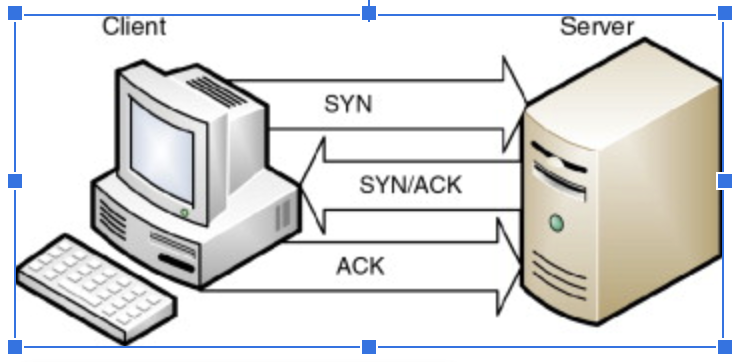
\includegraphics[width=\linewidth]{figures/tcp_handshake.png}
    \caption{\gls{tcp}’s Three-Way Handshake}
    {Source: ADD SOURCE}
    \label{figure:tcp_handshake}
\end{figure}

The sender chooses the initial sequence number, informed in the first \gls{syn} packet. The receiver also chooses its own initial sequence number by informing in the \gls{synack} sent to the sender. Each side acknowledges each other’s sequence number by incrementing it, allowing both sides to detect missing or out-of-order segments \cite{telecom_network_security}.

\gls{tcp} is stream oriented, effectively meaning it has the ability to send or receive a stream of bytes \cite{rfc793}. It can bundle up data that comes from the application layer and send it in a single segment, being responsible for breaking the stream of data into segments, and reassembling once they reach the other side. \gls{udp}, on the contrary, is a message-oriented protocol where the division of data into user datagrams is made by the application \cite{data_networks_ip}.

To be able to offer more functionality, \gls{tcp} ends up sacrificing efficiency. While in the case of a connectionless and unreliable protocol such as \gls{udp}, it turns out to be faster due to the lack of any extra features \cite{tcp_udp_comparison}.

\subsection{TLS}

As more people have access to the Internet, the higher the requirement is for it to be secure. Data generated by users can have many harmful implications since it is directly related to privacy. While offering reliability, which is a necessary attribute to Internet’s communication, \gls{tcp}’s communication is not encrypted. Therefore, anyone with a minimum knowledge of networking can see everything that’s traversing the network, breaking with users' privacy.

The \gls{tls} protocol is a cryptographic protocol designed to provide privacy and data integrity between two communicating applications \cite{rfc5246}. The connection is considered private since symmetric cryptography is used for data encryption and every connection has an unique generated key negotiated between parties.

Peers' identity can be authenticated through the use of asymmetric cryptography \cite{auto_verification_tls_handshake}. This is important because both sender and receiver can establish a trusted relationship by verifying if their certificates and public IDs are valid and have been issued by a \gls{ca} listed in their respective list of trusted \gls{ca}s.

To be able to establish a \gls{tls} connection, the sender and receiver must negotiate a connection by doing a \gls{tls} handshake. It allows hosts to authenticate with each other and to negotiate a cipher and generate session keys in order to use symmetric encryption before the application protocol actually starts to transmit data.

\gls{tls} can be used to encrypt \gls{tcp} connections by including the \gls{tls} handshake to \gls{tcp}’s connection establishment flow (Figure \ref{figure:tls_handshake}). This adds an overhead by increasing the number of \gls{rtt} needed before the actual data transmission starts.

\begin{figure}[ht]
    \centering
    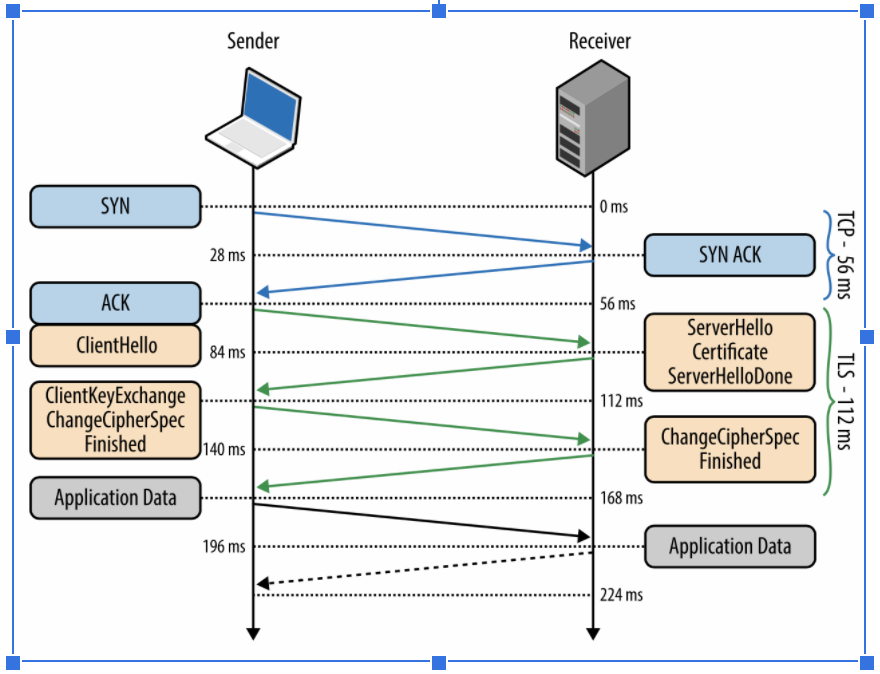
\includegraphics[width=\linewidth]{figures/tls_handshake.png}
    \caption{\gls{tls} Handshake}
    {Source: ADD SOURCE}
    \label{figure:tls_handshake}
\end{figure}

Working alongside one another, \gls{tcp} and \gls{tls} have kept the Internet reliable and encrypted. However, they only provide the channel of communication, how applications communicate is determined by the application-layer protocols.

\subsection{HTTP}

The \gls{http} is considered the foundation of the World Wide Web. It is an application-level protocol for distributed, collaborative, hypermedia information systems that runs on top of the other layers in the network protocol stack \cite{rfc1945, rfc2616, what_is_http}.

It is a generic, stateless protocol which uses a predefined set of standards and rules for exchange of information through a request-response process \cite{rfc1945, rfc2616}. The sender submits an \gls{http} request message to the receiver, which provides resources, such as \gls{html}, or performs some action on behalf of the sender. The receiver then returns a response message to the sender, it contains status information about the request and possibly the requested data in the message body, enabling the sender to react in a proper way, either by moving on to another task or handling an error \cite{rfc2616}.

The following subsections introduce \gls{http} versions, what they improved and a general feeling of how they work.

\subsection{HTTP/1}

The first version of \gls{http}, known as \gls{http}/0.9, was a simple protocol for raw data transfer across the Internet \cite{rfc2616}. It only had the GET request method, equivalent to a request to retrieve data from the server. Message types were limited to text, and it had no \gls{http} headers, meaning there was no metadata, such as status or error codes, on the request/response.

\gls{http}/1.0 improved the protocol by allowing messages to support the \gls{mime} standard, which extends data types supported by messages, being possible to send videos, audio, and images \cite{rfc2616}. In addition, metadata was also incorporated into requests and responses, increasing the available request methods, while improving error handling by the use of status and error codes.

\gls{http}/1.1 is considered a milestone in the evolution of the Internet, since it eliminates a lot of problems from previous versions and introduces a series of optimizations \cite{what_is_http}. Connections can be reused in favour of having to create a connection to every request and can be pipelined, improving the time needed to perform multiple requests. It also provides support for chunked transfer, which is a streaming data transfer mechanism that divides the data stream into “chunks” that are sent out independently of each other. This allowed for a more efficient transfer of large amounts of data due to concurrency.

\subsection{HTTP/2}

\gls{http}/2 purpose is to optimize transport for \gls{http} semantics, while keeping the support for all of the core features of the \gls{http}/1.1.

Even though \gls{http}/1.1 added pipelined connections, it still suffers from the Head of Line blocking (HOL blocking) problem \cite{rfc7540}. It happens when the number of allowed parallel requests is used up, and subsequent requests need to wait for the former ones to complete. \gls{http}/2 solves this by implementing multiplexing. This is achieved by having \gls{http} request/response associated with its own stream and since streams are independent of each other, a blocked request/response does not prevent progress on other streams.

\gls{http}/2 adds a new interaction mode where a receiver can push responses to the sender \cite{rfc7540}. This resulted in senders not needing to send periodical requests for new data to the server by using polling methods, trading network usage for some improvement in latency.

Because \gls{http} header can contain a lot of redundant data, \gls{http}/2 uses a compressed binary representation of metadata instead of a textual one, this reduces the space required \cite{rfc7540}.

\subsection{HTTPS}

\gls{https} is an extension of \gls{http}, conceptually equivalent to \gls{http} over \gls{tls} \cite{rfc2818}. \gls{https} is when the \gls{http} client also acts as a \gls{tls} client, it should perform all \gls{tls} requirements, such as establishing a connection through a \gls{tls} handshake. Once it finishes, the client may initiate the first \gls{http} request, the difference being all data will be encrypted. \gls{https} maintains \gls{http} behaviour while providing \gls{tls} features for instance encryption, data integrity, and authentication \cite{rfc2818}.

\subsection{QUIC}

\gls{https} provides a reliable and secure connection and is considered the main application-layer protocol used by the World Wide Web. However, it has some limitations due to requiring the use of \gls{tls} for security and \gls{tcp} for reliability.

QUIC is a secure general-purpose transport protocol designed to improve performance for \gls{https} traffic and to enable rapid deployment and continued evolution of transport mechanisms \cite{quic_protocol}. It replaces most of the traditional \gls{https} stack: \gls{http}/2. \gls{tls}, and \gls{tcp} (Figure \ref{figure:quic_http2_layers}).

\begin{figure}[ht]
    \centering
    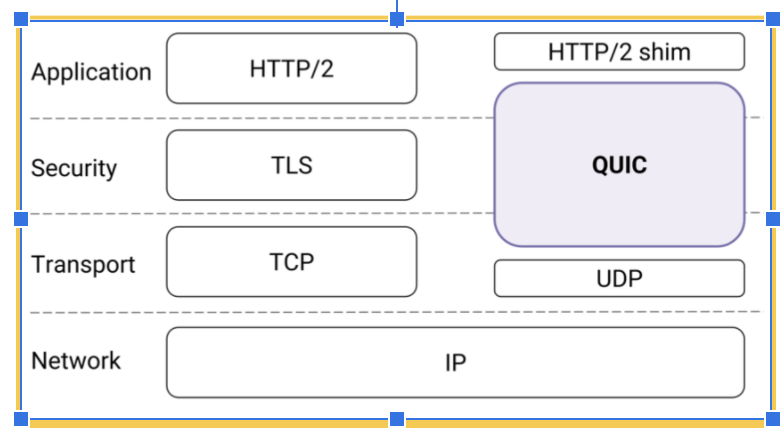
\includegraphics[width=\linewidth]{figures/quic_http2_layers.png}
    \caption{\gls{https} vs QUIC Layers}
    {Source: ADD SOURCE}
    \label{figure:quic_http2_layers}
\end{figure}

As the Internet evolves, software requires fast deployment of changes both to improve and to secure it. \gls{tcp} is a kernel-space transport protocol, meaning that any vulnerabilities or improvements require an upgrade to the \gls{os} kernel. Since such changes have a huge impact on the entire system, they must be made with caution and may take years to become widely spread \cite{rfc9000}. QUIC was developed as a user-space transport protocol on top of \gls{udp}, facilitating its deployment as part of other applications, resulting in meaningful impact in a relatively short time \cite{quic_protocol}.

A middlebox is when a device adds functionality other than packet forwarding to an IP router, such as filtering, altering, and manipulating traffic \cite{rfc3234}. Improvements to transport protocols is reduced due to the fact that these kinds of devices are hard to be removed or upgraded, creating a dependency between them. For example, firewalls tend to block any unknown traffic for security reasons, meaning that new transport protocols need to be explicitly supported \cite{rfc3234}. QUIC addresses this issue by encrypting its packets, therefore avoiding middlebox dependency and data tampering \cite{quic_protocol}.

gls{http}/2 solves the HOL blocking problem in the application layer by introducing request multiplexing, however it still suffers from this problem in the transport layer. Even though \gls{http}/2 streams are independent of each other, they still had to share a \gls{tcp} connection and deal with \gls{tcp}’s window size. If the first window segment fails, the window cannot go further and blocks new segments from being transmitted. QUIC solves this problem by implementing stream multiplexing. More than one stream within a connection means that even if one stream drops packets, other streams will not be blocked in any way.

\gls{https} is required to perform both \gls{tcp} and \gls{tls} handshakes to establish a secure connection, resulting in generally a 3-\gls{rtt} connection setup (Figure \ref{figure:tcp_v_tls_v_quic_handshake}) to be able to start transmitting the actual data \cite{rfc7413}.

\begin{figure}[ht]
    \centering
    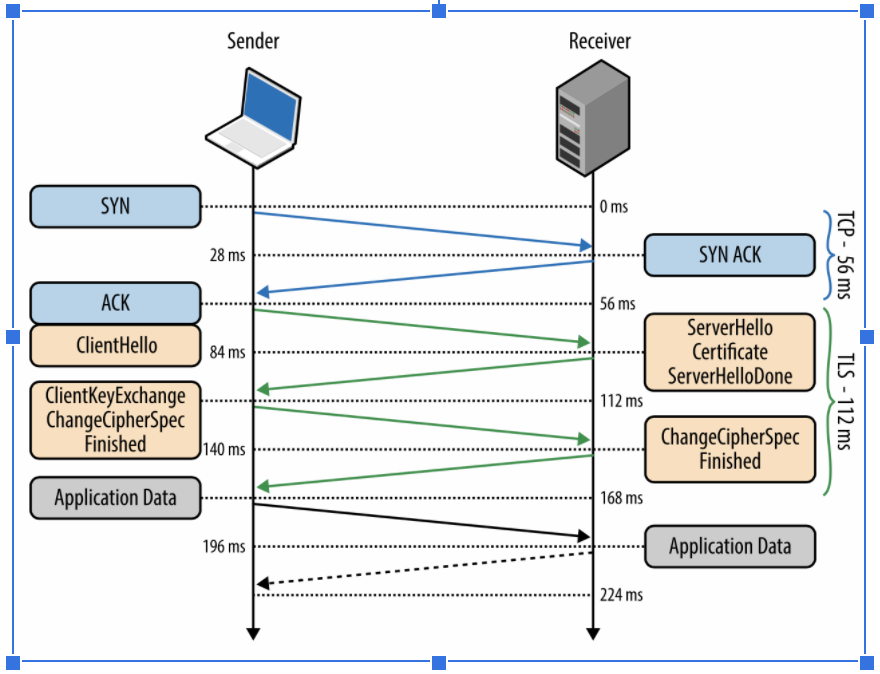
\includegraphics[width=\linewidth]{figures/tls_handshake.png}
    \caption{\gls{tls} Handshake}
    {Source: ADD SOURCE}
    \label{figure:tcp_v_tls_v_quic_handshake}
\end{figure}

QUIC improves the handshake delay by minimizing the steps required to establish a connection, being able to perform a 0-\gls{rtt} connection setup once the server is known (Figure \ref{figure:quic_handshake}) \cite{quic_protocol, rfc9000}. It does this by caching information about the server on the client after a successful connection. If it tries to set up a connection with expired information, the server sends a reject message that contains all the information necessary to establish a connection.

\begin{figure}[ht]
    \centering
    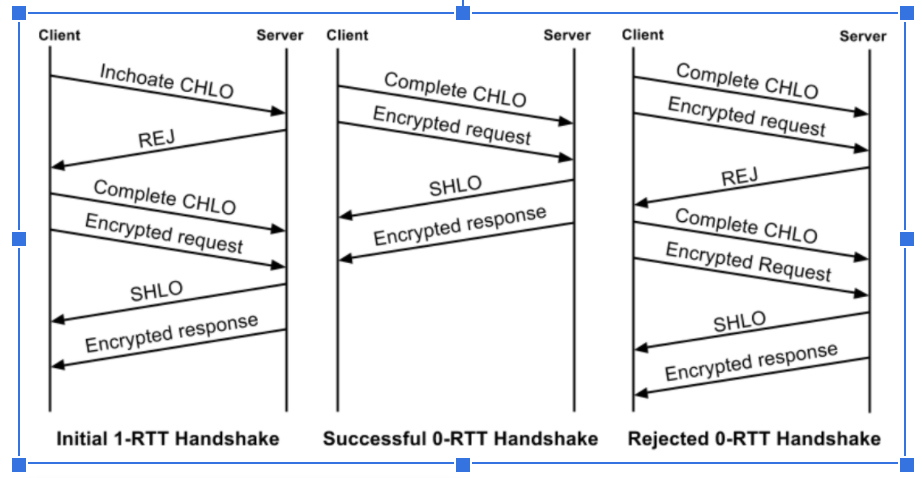
\includegraphics[width=\linewidth]{figures/quic_handshake.png}
    \caption{QUIC Handshake}
    {Source: ADD SOURCE}
    \label{figure:quic_handshake}
\end{figure}

\gls{tcp} loss recovery mechanisms are able to detect when a segment is probably dropped, triggering its retransmission. This process uses \gls{rtt} estimation to improve its efficiency, which in the case of \gls{tcp}, is based on \gls{tcp}’s sequence numbers. However, once a retransmission is made, there is no way of knowing if the \gls{ack} received is for the original or the retransmitted segment since both segments use the same sequence number. Additionally, dropped retransmission segments are usually detected by the use of timeouts, further slowing \gls{tcp} \cite{quic_protocol,rfc2988,rfc9000,tcp_timer_dont_work_well}.

QUIC eliminates \gls{tcp}’s retransmission ambiguity problem by including a new packet number to all packets, even those including retransmitted data \cite{rfc9000}. This means it can measure \gls{rtt}s precisely since it always knows which packet each \gls{ack} refers to. To maintain the data order, QUIC adds a stream offset to the stream frames present in the packet, decoupling the need of ordered packet numbers \cite{quic_protocol}.

While QUIC improves transport efficiency, it demands more computational resources when compared to \gls{tcp}+\gls{tls}. The focus during its design was improving transport, not resource efficiency, resulting in an initial raise by 3.5 times of \gls{cpu} utilization when compared to \gls{tcp}+\gls{tls} traffic \cite{quic_protocol}. Optimizations were made after this assessment, decreasing \gls{cpu} usage difference to 2 times \gls{tcp}+\gls{tls}’.

\subsection{HTTP/3}

\gls{http}/3 is effectively \gls{http} over QUIC. It provides a transport for gls{http} semantics using QUIC as transport protocol, therefore it maintains all the same request methods, status codes, and messages fields. It still does not have an official \gls{rfc}, however it possesses an initial draft [32]. Nonetheless, it is supported by 74% of running web browsers, Google Chrome being one of them [33].

\subsection{Summary}
<INSERT>

\clearpage

\section{Background in Distributed Systems on Cloud}

The previous section introduced the QUIC protocol and all protocols that it’s either trying to improve, or their previous versions. Their differences and motivations were defined and will be used to explain the results of the experiments described further ahead.

In order to understand the experiment's motivations, this section provides an overview of the challenges to build distributed applications on cloud and what they offer to be used in production environments by many large scale companies.

\subsection{Distributed Systems}

Back in the day, the most common way to solve a computing problem was to write a single application that was responsible for performing some kind of task. These applications are called monolithic applications.

Once the application grows to a point it demands scaling, it will demand more replicas of itself to be able to handle more traffic. Though this might not be a problem, since all functionality was incorporated into a single application, in most cases, only a few parts will actually require scaling. Consequently, resulting in a waste of resources.

Distributed systems come into the scene to try solving these problems. It makes use of multiple computing devices spread over a network and have them coordinate efforts to perform some kind of task \cite{distributed_systems_principles}. It allows complex applications to be broken down into manageable chunks, each performing a different kind of functionality.

Its components can be broken down into two categories of clients: ephemeral and persistent.

An ephemeral client creates a single connection to the server, performs some sort of exchange of data, and then closes the connection once it’s finished. A common example is that of a job, a finite task that has to perform a large computation, batch-oriented tasks, or creating a database backup \cite{os_distributed_systems}.

A persistent client, however, also establishes a single connection to the server, but it maintains it open throughout its entire lifetime, making requests when needed. This can be represented by a service that needs to communicate with a database to provide some kind of functionality.

By defining these components and how they work, simulations can be performed to see how they perform on different scenarios. This allows for speculation about their behaviour in a real-world scenario.

\subsection{Cloud}

The term “cloud” was used to refer to platforms for distributed computing as early as 1993 \cite{what_is_cloud}. Cloud computing the delivery of computing services, such as databases and storage, over the Internet. It can be divided into three main categories: \gls{iaas}, \gls{paas}, and \gls{saas}. From here on, the focus will be the \gls{iaas} cloud computing category.

\subsubsection{\gls{iaas} \& Containerization}

\gls{iaas} is a form of cloud computing that has become one of the most common ways to provision on-demand availability of infrastructure services without having to be directly managed by the user \cite{what_is_cloud}.

Users are not required to have their own data centers to be able to serve their applications, they can request resources to use a third party’s computing infrastructure using a pay-as-you-go method. Therefore, they only need to pay for the resources actually used, enabling them to easily scale when needed.

Multi regional servers are also possible. Users are able to request resources in distinct regions to deal with traffic from different countries or due to some contractual requirements. Some providers even have more than one data center per region, capaciting users to build high availability systems that are able to deal with disaster scenarios, for instance the data center experiences a power outage.

As data centers machines processing power and capacity increased over the years, many resources never got to be used by the applications whereas their requirements were much lower. This causes a waste of computing resources that could otherwise be used by users, increasing providers’ revenue. Thus, \glspl{vm} came into existence. 

\gls{vm}s consist of the virtualization of an \gls{os}, allowing one single physical host machine to have more than one virtual machine running at the same time while keeping them isolated from each other \cite{what_is_cloud}. This enables cloud providers to optimize the use of their resources by serving multiple \gls{vm}s while only having to use one physical host machine, consequently serving more than one user per machine.

Nevertheless, \gls{vm}s improve data centers resource efficiency, it can take up a lot of system resources. Each \gls{vm} requires a copy of an \gls{os} and a virtual copy of all the hardware that the \gls{os} needs to run, adding up to a lot of memory and \gls{cpu}. This is still more efficient than running separate physical host machines, but can be a deal-breaker for applications.

To improve application development, deployment and flexibility, containers were created. Instead of virtualizing the entire host machine, containers use linux namespaces to run on isolated environments while sharing the underlying \gls{os} (Figure \ref{figure:vm_vs_container}), resulting in less requirements since they only need to package the actual application and all files necessary to run. In addition, their lightweight characteristic allows faster startup time, while \gls{vm}s may take minutes to be provisioned, most containers are ready in a few milliseconds.

\begin{figure}[ht]
    \centering
    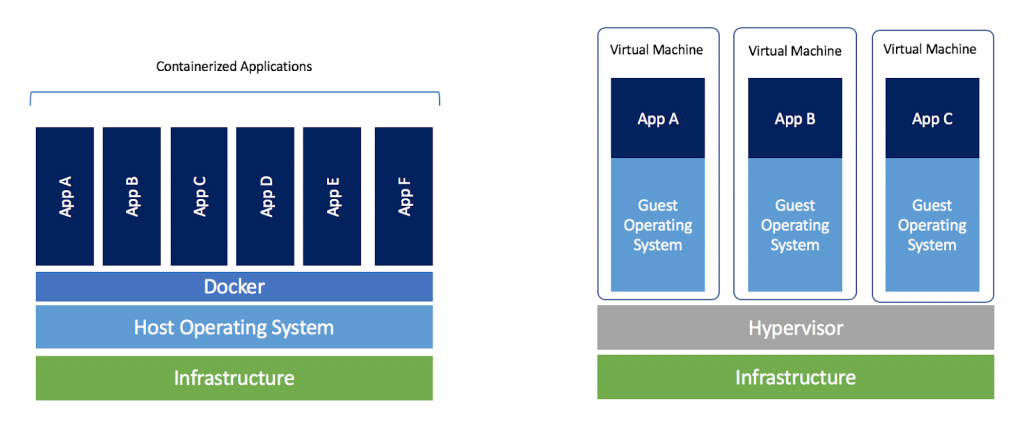
\includegraphics[width=\linewidth]{figures/Blog.-Are-containers-..VM-Image-1-1024x435.png}
    \caption{Containers versus Virtual Machines}
    {Source: \cite{are_containers_replacing_virtual_machines}}
    \label{figure:vm_vs_container}
\end{figure}

Developers usually write code locally possibly using their laptop, and then this code will be deployed on the server. Any differences between these two environments, laptop and server, can cause unexpected bugs. Containers solve the problem of environment inconsistency. Developers can work on a local environment that contains all of the dependencies of any environment whether it’s development, testing, or production.

\subsubsection{Kubernetes}

Dealing with distributed systems over the cloud have given companies the power to build complex and intelligent solutions that are able to solve really hard problems that otherwise would require a lot of investment and time. However, managing such systems comes with its own challenges.

Due to containers being lightweight and ephemeral, running them in a production environment can become overwhelming. A containerized application might need to operate hundreds to thousands of containers. A container orchestrator is the automation of operational effort required to run such containerized applications.

According to the \gls{cncf}, \gls{k8s} is an open source container orchestration engine for automating deployment, scaling, and management of containerized applications \cite{kubernetes}. Additionally, it’s considered the most widely used container orchestration platform by \gls{cncf}’s \gls{k8s} Project Journey Report from 2019 \cite{cncf_k8s_report}.

The fundamental premise behind \gls{k8s} is that it enforced desired state management. Consequently, a \gls{k8s} cluster is fed with specific configuration files, called manifests, and it's up to the cluster to provide the necessary infrastructure to be able to meet the desired state.

\gls{k8s}’ smallest and most basic deployable object is called pod. It consists of a wrapper around containers that has computing resources. One or more containers can be inside a single pod, consequently sharing the pod’s resources with each other.

In the context of containers, a pod is a set of Linux namespaces and the same things that are used to isolate a container. Therefore, in the context of \gls{k8s}, it’s common to refer to pods when talking about scaling and deployment.

Each cloud provider often provides a managed way of running \gls{k8s}, they take care of the control plane, component responsible for managing the worker nodes and the pods, management while enabling users to actually use the cluster to their needs. For instance, \gls{aws} offers the \gls{eks}.

Some cloud providers allow applications to be deployed in different regions. In the case of \gls{aws}, it even allows you to choose a data center within a region, defined as \gls{az}. Hence, there can be multiple \gls{az}s within a single region.

Within the \gls{k8s} it’s possible to have pods deployed to different regions or \gls{az}s based on their affinity and tolerations by tainting a node with a label. This allows the user to have full control over where each application is going to run.

\subsection{Summary}

This section finished all required aspects of managing distributed systems on cloud. Therefore, their challenges and benefits should be clear, as well as their importance to the computing world.

The next section will bring details on how the implemented Benchmark Service will perform experiments. They are going to put previously described protocols to the test in a cloud environment. Consequently, being able to assess their results.

\clearpage

\section{Experiments Setup}

This section explains the reasons for each experiment's characteristics, why each scenario is considered, what they bring to the table, and what kind of metrics are going to be collected.

\gls{udp}, \gls{tcp}, \gls{tcp}+\gls{tls} and QUIC transport-layer protocols will be compared. In addition, \gls{http}/1, \gls{http}/1+\gls{tls}, \gls{http}/2, \gls{http}/2+\gls{tls} and \gls{http}/3 application-layer protocols will also be compared.

Ephemeral and persistent clients are going to be used, each running in three scenarios:
\begin{itemize}
    \item Multi-AZ, different nodes in different \gls{az}s
    \item Same-AZ, different nodes in the same \gls{az}
    \item Local, same node
\end{itemize}

Persistent clients are used in two kinds of experiments: sequential and concurrent. The former simulates clients that are able to maintain a connection, but are only able to send one request at a time in a sequential manner. The concurrent experiments, however, simulates most services, which are able to maintain a connection and perform multiple requests simultaneously. These connections are limited to a maximum of 100 simultaneous requests.

All experiments will be performed in a \gls{k8s} Cluster deployed on \gls{aws} using \gls{eks}. Metrics collected will be:
\begin{itemize}
    \item Latency
    \item Throughput
    \item \gls{cpu}
    \item Memory
\end{itemize}

All experiments are executed using a simple demo application that implements every protocol in the most efficient and similar way. It is a simple application since all it does is establish a connection with the server, send a fixed amount of data, wait and receive its response, and, depending on the type of client, either close the connection or keep sending requests.

The fool

\subsection{About Protocols}

Since QUIC is a transport-layer protocol, it makes sense to compare it with other protocols from the same layer. This enables observation on how they perform under the same circumstances.

QUIC replaces most of the \gls{https} stack: \gls{http}/2, \gls{tls}, and \gls{tcp}. Therefore, it will be compared against \gls{udp}, \gls{tcp}, and \gls{tcp}+\gls{tls} transport protocols.. By making this comparison only in the transport layer, there will be less variables to consider when analysing the results.

Since QUIC uses \gls{udp} as part of its implementation, it is also considered, as it might show how effectively it’s used by QUIC.

\gls{udp} is used in its pure implementation, therefore no additional logic is incorporated to be able to grasp its performance. This means there might be scenarios in which it will not be able to successfully finish experiments due to its unreliable nature.

In addition, \gls{http}/3, also known as \gls{http} over QUIC, will be compared against its predecessors: \gls{http}/1 and \gls{http}/2. Comparing application-layer protocols enables us to observe QUIC’s impact on a real-world situation, since applications will not use QUIC directly, but through \gls{http}. Furthermore, QUIC also performs \gls{tls}’ role of securing \gls{http}’s traffic, therefore \gls{http}/1+\gls{tls} and \gls{http}/2+\gls{tls} protocols will also be tested.

\subsection{About Clients}

By separating clients into persistent and ephemeral categories, experiments are able to simulate two very common scenarios on distributed systems and observe how QUIC behaves when having to deal with each one of them.

The first scenario explores ephemeral connections, representing when we have a job that needs to perform some sort of finite task, creating a single connection to the server, and closing it once it’s done.

The second scenario explores persistent connections, representing when we have a service that needs to communicate with a database to provide some kind of functionality, creating a single connection to the database throughout its entire lifetime.

\subsection{About Kubernetes}

All experiments are made inside a \gls{k8s} Cluster since it is a production-grade container orchestrator, a common production environment used by most companies that have to deal with container management in the cloud.

By choosing to use this environment, it not only reflects an actual production scenario, but also allows easy networking setup for nodes running on different \gls{az}s. Running nodes on different \gls{az}s is a requirement due to high availability, as every data center is always under the danger of downtime due to a natural disaster or to some event that damages some of the datacenter’s infrastructure. Therefore, Multi-\gls{az} is a must have for companies that require a disaster recovery plan to be able to deal with such catastrophic events.

During the experiments, three scenarios are taken into account: when the client and server are running in the same node, when they are running in different nodes while in the same \gls{az}, and when they are running in different nodes while in different \gls{az}s. These are all possible scenarios when using \gls{k8s} since client and server applications may be running in any node, depending on the configuration.

To be able to control which nodes were going to be used by each application during experiments, pod affinity and taint were configured to be able either force a pod to be scheduled on required nodes.

During the local scenario, pod taint was used to make pods to be scheduled to a node in the same \gls{az}, and pod anti-affinity and affinity were used to make client and server pods to be scheduled to the same node. During the different nodes in the Single-\gls{az} scenario, pod taint was also used to schedule pods to nodes in the same \gls{az}, but only pod anti-affinity was used to make sure there was only one pod running in each node. The last scenario required pods to be running on nodes in different \gls{az}s, pod taint was used to schedule pods to different \gls{az}s, while pod-affinity was also used to make sure there was only one pod running in each node.

\subsection{About Metrics}

QUIC has an increased usage in memory and \gls{cpu} since the focus during development was performance and not efficiency, resulting in an initial raise by 3.5 times of \gls{cpu} utilization when compared to \gls{tcp}+\gls{tls} traffic [14]. Optimizations were made after this assessment, decreasing the \gls{cpu} usage to 2 times \gls{tcp}+\gls{tls}’, however it’s still believed that, even after more optimizations, this increased cost will always exist.

Latency and throughput are also analyzed to be able to grasp a better understanding on how performatic each protocol is in relation to how fast it can respond to requests and exactly how much data can be transmitted every second.

\subsection{About Demo Application}

Developed in Go, this demo application aims to implement every protocol used during these experiments in the most efficient and similar way.

Each protocol must implement an ephemeral client, a persistent client and a server. 

The ephemeral client’s job is to establish a connection with the server, send a single request, wait for its response and close the connection, this can be performed multiple times, always resulting in a closed connection after a single request. 

The persistent client’s job is similar to the former, the only difference being multiple requests can be made within a single connection. Two kinds of experiments are performed with this type of client: sequential and concurrent. The former simulates clients that do not support concurrent requests, therefore is only able to send one request at a time. The concurrent experiment, otherwise, simulates services that are able to perform multiple requests at the same time. Microsoft states most gRPC servers set concurrent requests limit to 100 by default [27]. Therefore, this experiment set the same limit to be able to simulate a real-world scenario.

The server’s job is to receive a request, and send a response with a fixed amount of data in it.

The size of data sent within the requests and responses is predetermined in compilation time. This value varies in the following manner: 2KiB, 8KiB, 32KiB, 128KiB, and 512KiB. These values were chosen due to the fact that they are a reasonable size of data transfer amongst services running in the cloud. Kafka's maximum package size’s default value is 1MB, because packages with more than 10MB can affect the performance of the cluster [25]. gRPC limits incoming messages size to 4MB to help prevent it from consuming excessive resources [26].

\subsection{About \gls{aws}}

\gls{aws} is one of the most popular cloud providers, offering a wide range of services. It was used as a provider due to its accessible price and since it met all experiments requirements. For instance, it allows use of \gls{aws} \gls{ec2}, \gls{aws}’ equivalent to \gls{vm}, to perform experiments.

Pricing was also taken into account when preparing for experiments. \gls{aws} not only charges for the \gls{ec2} instance and \gls{eks}, but also for data transfer between \gls{az}s, resulting in a hefty cost when exchanging terabytes of data.

During each experiment, 10000 requests are made. Therefore, one of the Multi-\gls{az} experiments, transferring requests and responses with 512KiB of data of a single protocol, transfers a total of 9.77 GiB of data. \gls{aws} charges \$0.02 per GiB transferred between \gls{az}s, resulting in an approximate cost of \$0.20 per experiment. With 9 protocols, ephemeral client, and persistent client with sequential and concurrent scenarios, all Multi-\gls{az} experiments with 512KiB of data costs approximately \$5.28.

\gls{az}s utilized during experiments were us-east-1 (use1-az1) and us-east-1b (use1-az2). The latter was only used during Multi-\gls{az} testing, while other experiments only used use1-az1.

The \gls{ec2} instance type used during experiments was m6i.xlarge. Initial experiments were performed with the smallest instance m6i.large and \gls{cpu} limit on \gls{k8s} was set to 1 \gls{cpu} per pod. This, however, resulted in interfering with QUIC results since this protocol was suffering throttled. To avoid throttling, this \gls{cpu} limit was removed and \gls{ec2} instance type was changed to xlarge, which contains 2 \gls{cpu}s instead of 1, assuring the pod will have all computational power it needs to perform as intended.

\subsection{Summary}

<INSERT>

\clearpage

\section{Transport Protocols Experiments}

\clearpage

\subsection{Latency \& Throughput}

Charts on Figures \ref{fig:persistent_transport_latency}, \ref{fig:ephemeral_transport_latency}, \ref{fig:parallel_transport_latency}, \ref{fig:persistent_transport_throughput}, \ref{fig:ephemeral_transport_throughput}, \ref{fig:parallel_transport_throughput} represent the \gls{p90} of Latency and Throughput of all 10000 requests made by the persistent and ephemeral clients during the experiments.

Throughout these charts it is possible to observe an order pattern. Local experiments usually were more performatic when compared to Single-\gls{az} experiments. Additionally, the latter results were better than Multi-\gls{az} experiments due to the overhead from sending the datagram to another data center, even though remaining in the same region.

\gls{udp} Multi-\gls{az} and Single-\gls{az} experiments only succeeded on the first two iterations of each run when the data transferred was 2KiB and 8KiB. This was expected since pure \gls{udp} does not have any reliability and is expected to lose user datagrams along the way. As was stated before, no additional logic was added to \gls{udp} since this would interfere with the results because it would alter \gls{udp} natural behaviour.

Local \gls{tcp} experiment was by far the most efficient, with almost zero latency when connection was persistent, reaching approximately 19Gb/s of speed when transferring 512KiB of data per request. It outperformed \gls{udp}, that even though is considered faster due to its unreliability and connectionless characteristics, it only reached 2.8Gb/s in the same scenario. This happened because, while \gls{tcp} is stream oriented, which enables it to send a continuous stream of data with no overhead, \gls{udp} is message oriented.

Nonetheless, ephemeral clients demonstrated that establishing connections can have a significant impact on \gls{tcp}’s performance. Local \gls{tcp} latency went from 0.19ms to 1.79ms and throughput from 19Gb/s to 2.2Gb/s. Both results are still better than other \gls{tcp} and all \gls{tcp}+\gls{tls}’ experiments \gls{p90}, but brings them to a similar level.

It is possible to observe \gls{tls} encryption overhead on \gls{tcp} during persistent clients experiments. Furthermore, during ephemeral clients this overhead increases due to having to perform a \gls{tls} handshake before every request.

QUIC’s experiments were the worst, with almost 7 times slower than \gls{tcp}+\gls{tls}’ Multi-\gls{az} experiment (with persistent client) latency and throughput. This demonstrates \gls{tcp}+\gls{tls} performs better than QUIC on a reliable network, with a low packet loss rate. However, QUIC performs better than \gls{tcp}+\gls{tls} on an unreliable network.

QUIC’s specifically designed to be used in environments such as a wireless network or a mobile device, both which have a high tendency to lose packets, and to break \gls{tcp} connections. QUIC solves these problems by implementing a more efficient way to deal with retransmission of lost packets, improving its throughput, and having a 0-\gls{rtt} handshake, which deals with broken connections by removing the need to perform a \gls{tcp} and \gls{tls} handshake.

Consequently, QUIC’s results show it's not meant to be used on distributed systems. These environments are usually part of a reliable network, meaning that \gls{tcp} is usually a better fit.

\subsection{Parallel}

All previous experiments performed requests sequentially, undermining the possible gain in efficiency of protocols that contain improvements to concurrent requests. Therefore this experiment tries to explore this scenario by performing all 10000 requests with 100 Goroutines, each performing 100 requests.

However, when packet size is the same, we fallback to a scenario where multiplexing is useless since any request performed in sequence is going to take more than the previous to complete. Therefore, this is similar to a pipelining scenario, where the requests finish in the order they were made.

\begin{figure}[h]
    \centering
    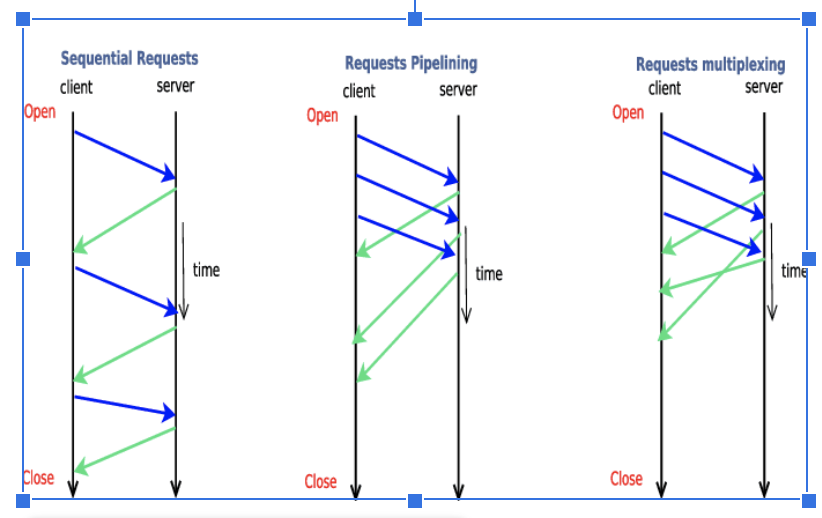
\includegraphics[width=\linewidth]{figures/pipelining.png}
    \caption{Pipelining}
    \label{fig:pipelining}
\end{figure}

\clearpage

\begin{figure}[h!]
    \centering
    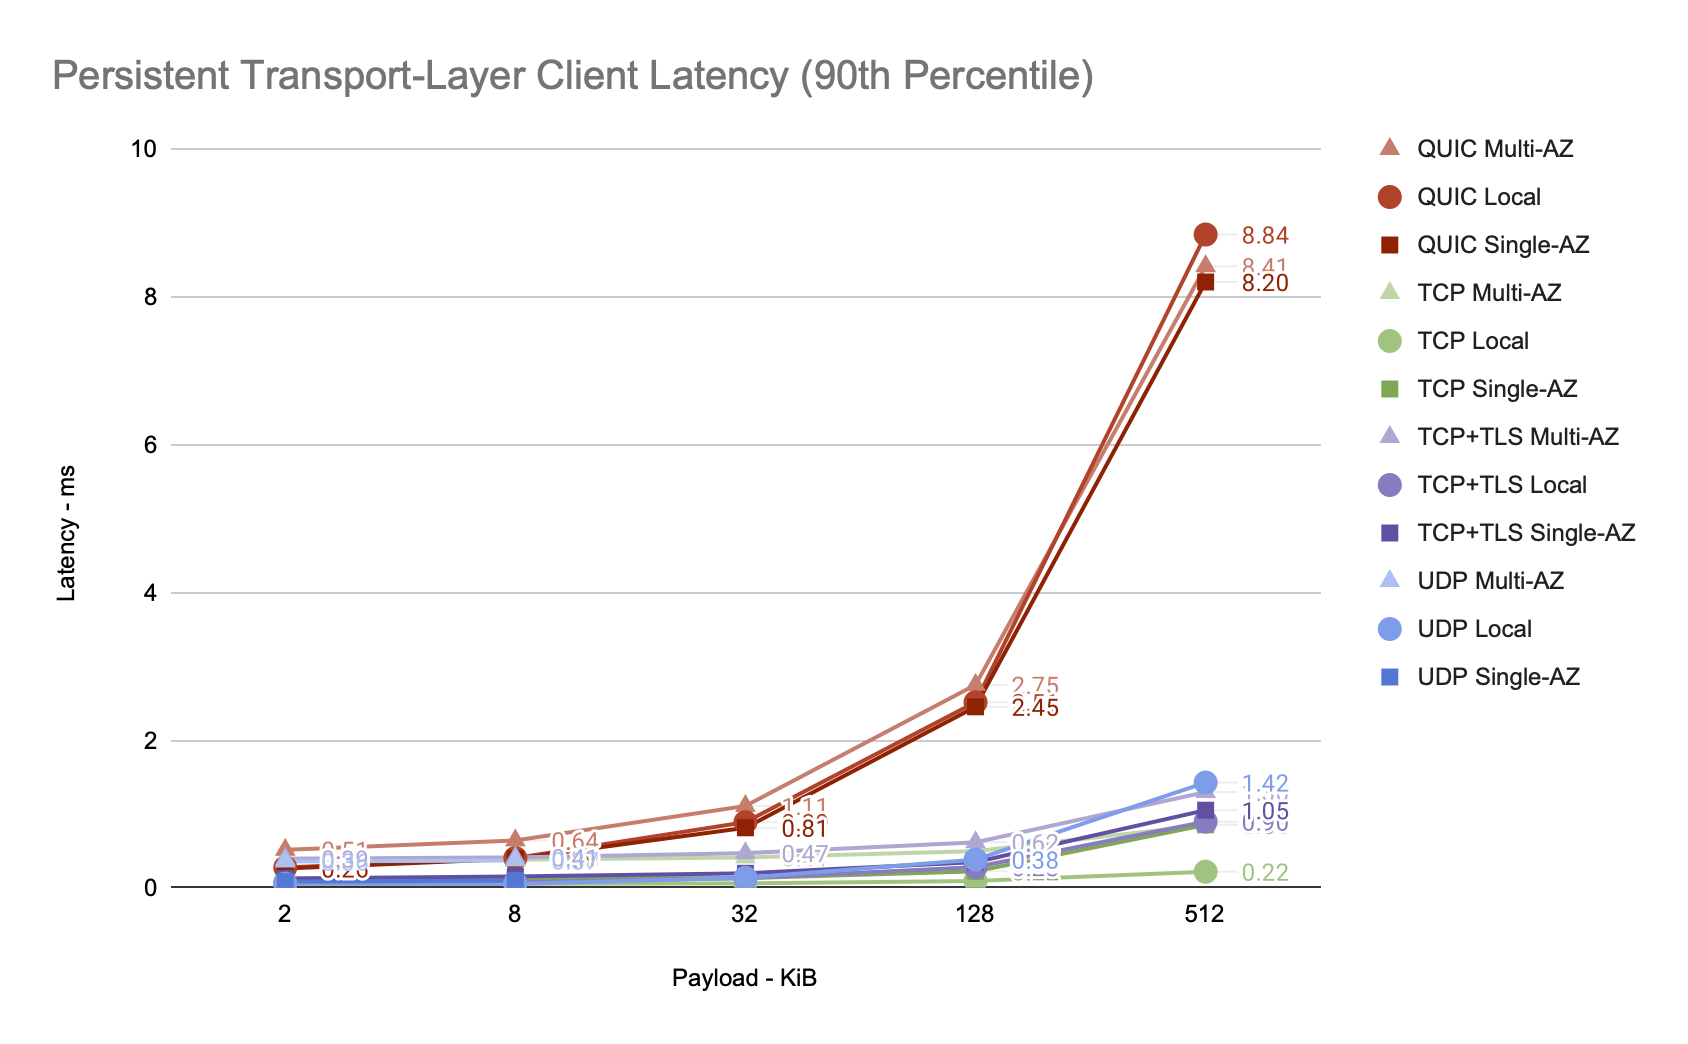
\includegraphics[width=\linewidth]{figures/charts/Persistent Transport-Layer Client Latency (90th Percentile).png}
    \caption{Persistent Transport-Layer Client Latency (90th Percentile)}
    \label{fig:persistent_transport_latency}
\end{figure}

\begin{figure}[h!]
    \centering
    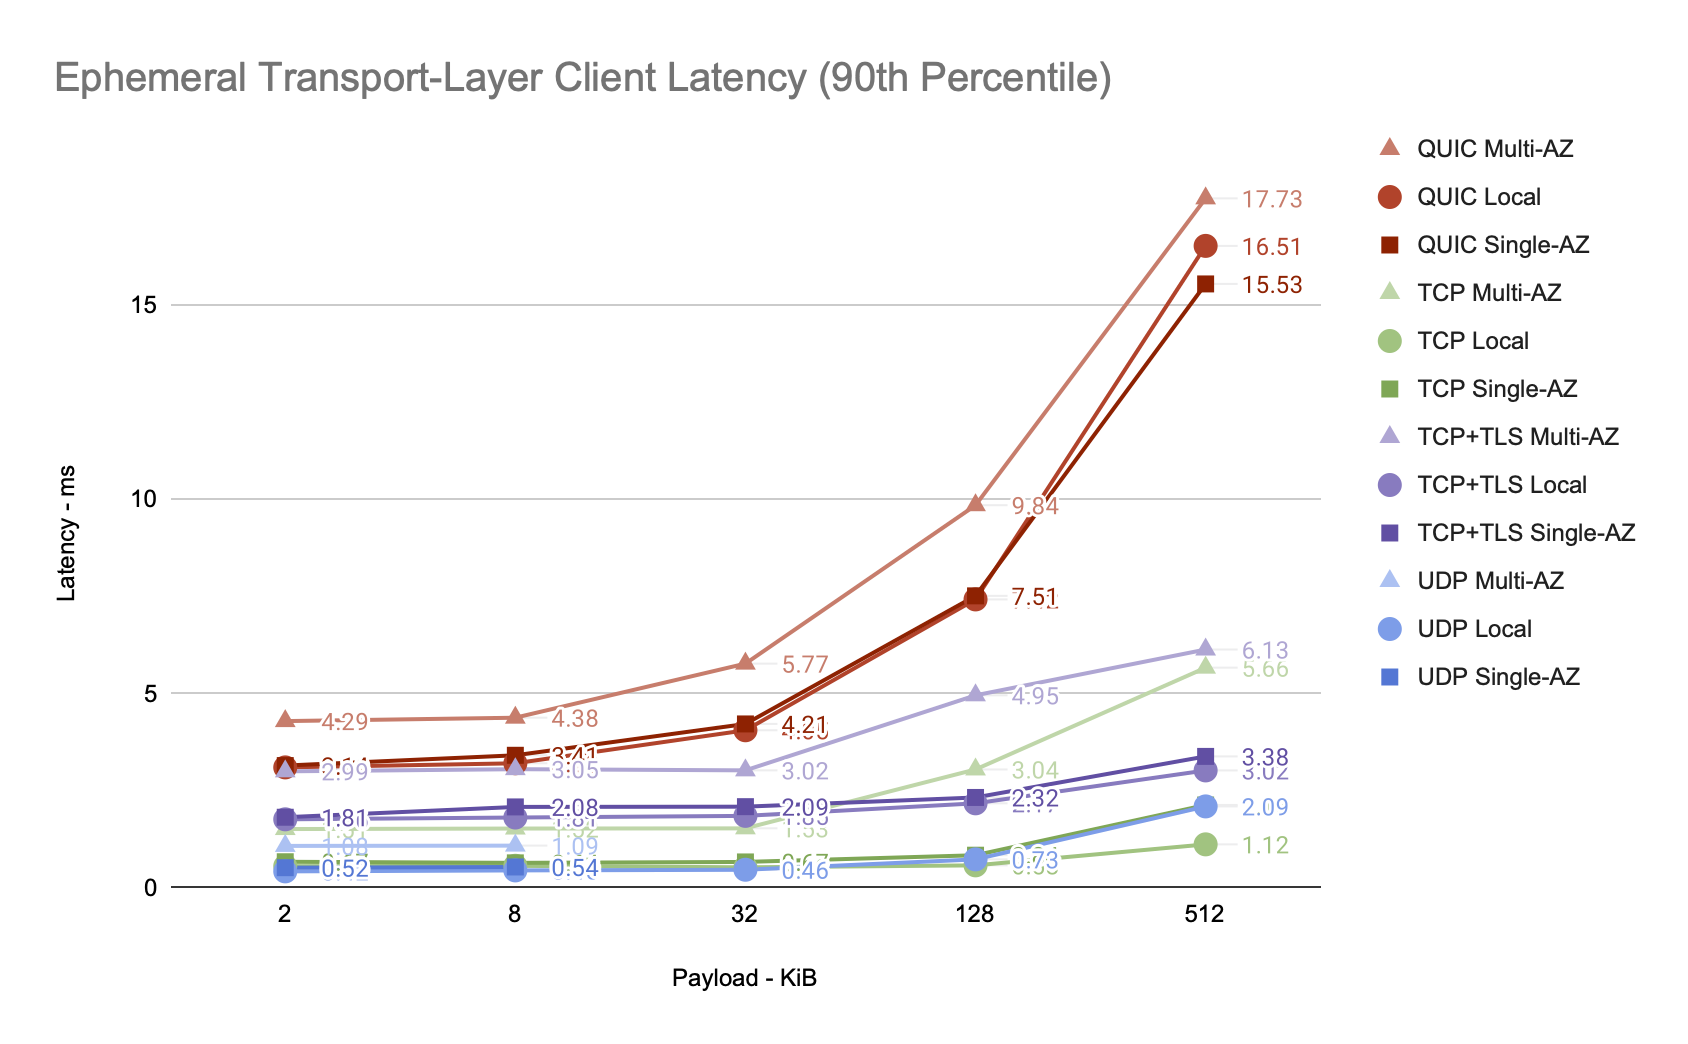
\includegraphics[width=\linewidth]{figures/charts/Ephemeral Transport-Layer Client Latency (90th Percentile).png}
    \caption{Ephemeral Transport-Layer Client Latency (90th Percentile)}
    \label{fig:ephemeral_transport_latency}
\end{figure}

\begin{figure}[h!]
    \centering
    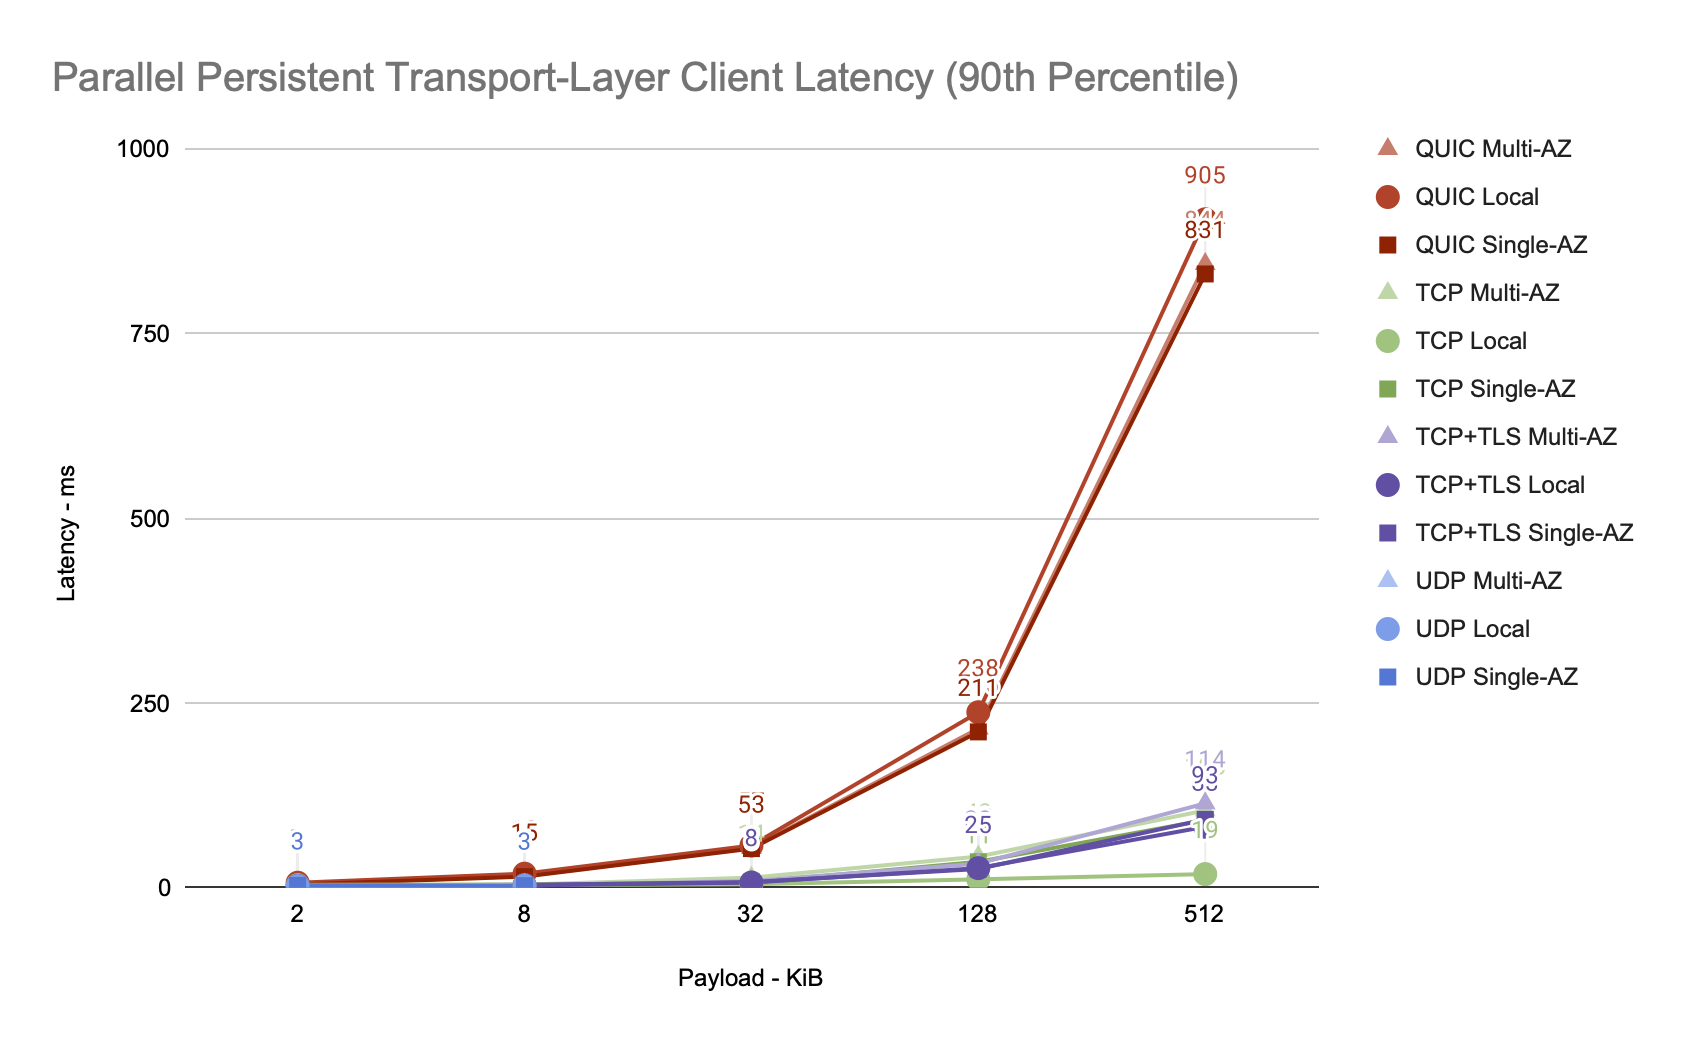
\includegraphics[width=\linewidth]{figures/charts/Parallel Persistent Transport-Layer Client Latency (90th Percentile).png}
    \caption{Parallel Persistent Transport-Layer Client Latency (90th Percentile)}
    \label{fig:parallel_transport_latency}
\end{figure}

\begin{figure}[h!]
    \centering
    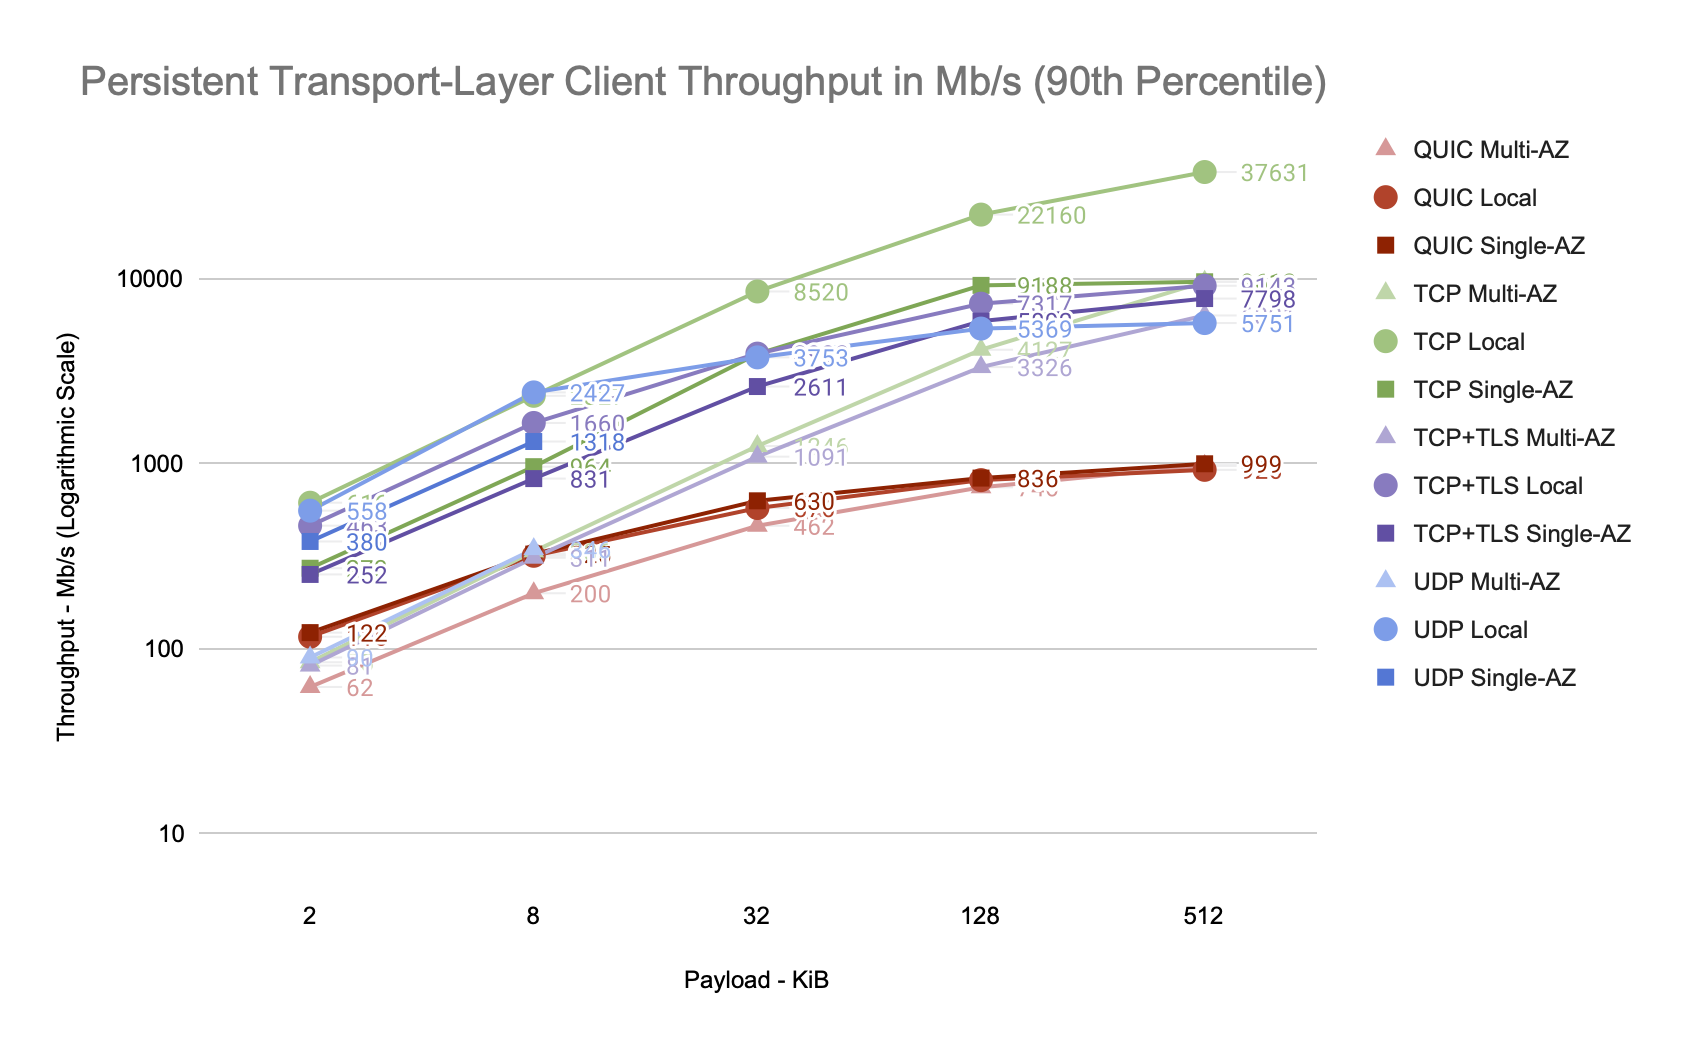
\includegraphics[width=\linewidth]{figures/charts/Persistent Transport-Layer Client Throughput in Mb_s (90th Percentile).png}
    \caption{Persistent Transport-Layer Client Throughput in Mb/s (90th Percentile)}
    \label{fig:persistent_transport_throughput}
\end{figure}

\begin{figure}[h!]
    \centering
    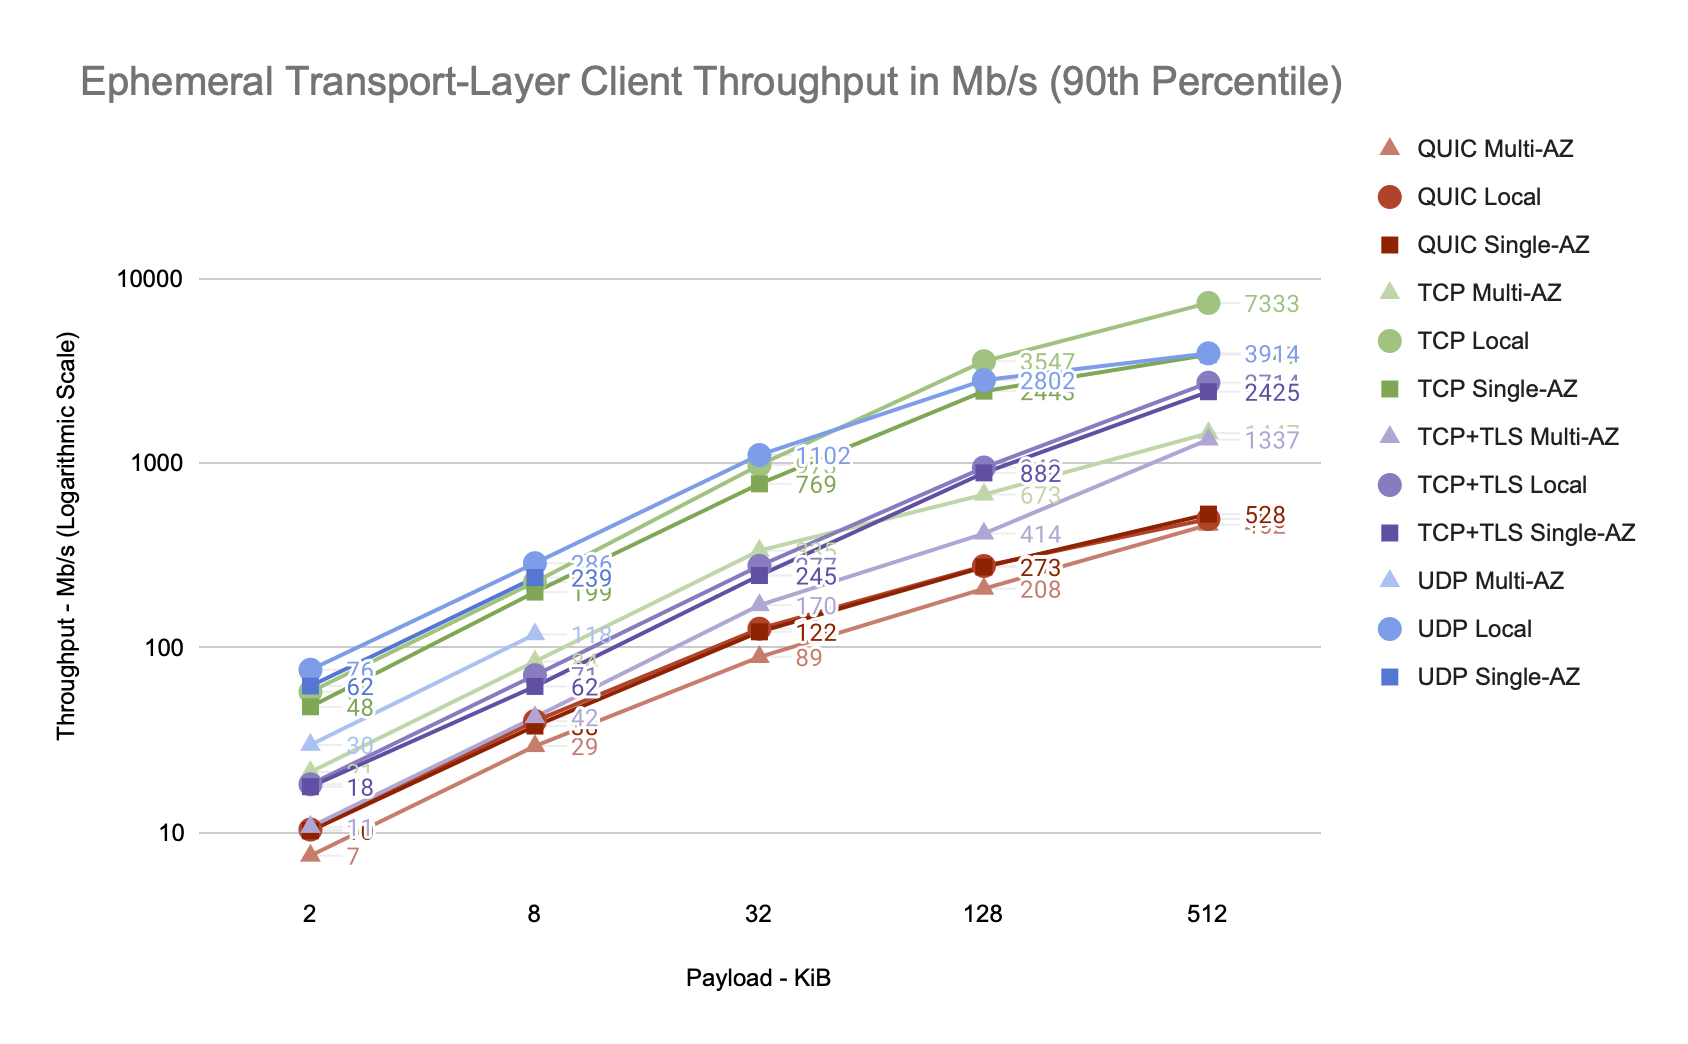
\includegraphics[width=\linewidth]{figures/charts/Ephemeral Transport-Layer Client Throughput in Mb_s (90th Percentile).png}
    \caption{Ephemeral Transport-Layer Client Throughput in Mb/s (90th Percentile)}
    \label{fig:ephemeral_transport_throughput}
\end{figure}

\begin{figure}[h!]
    \centering
    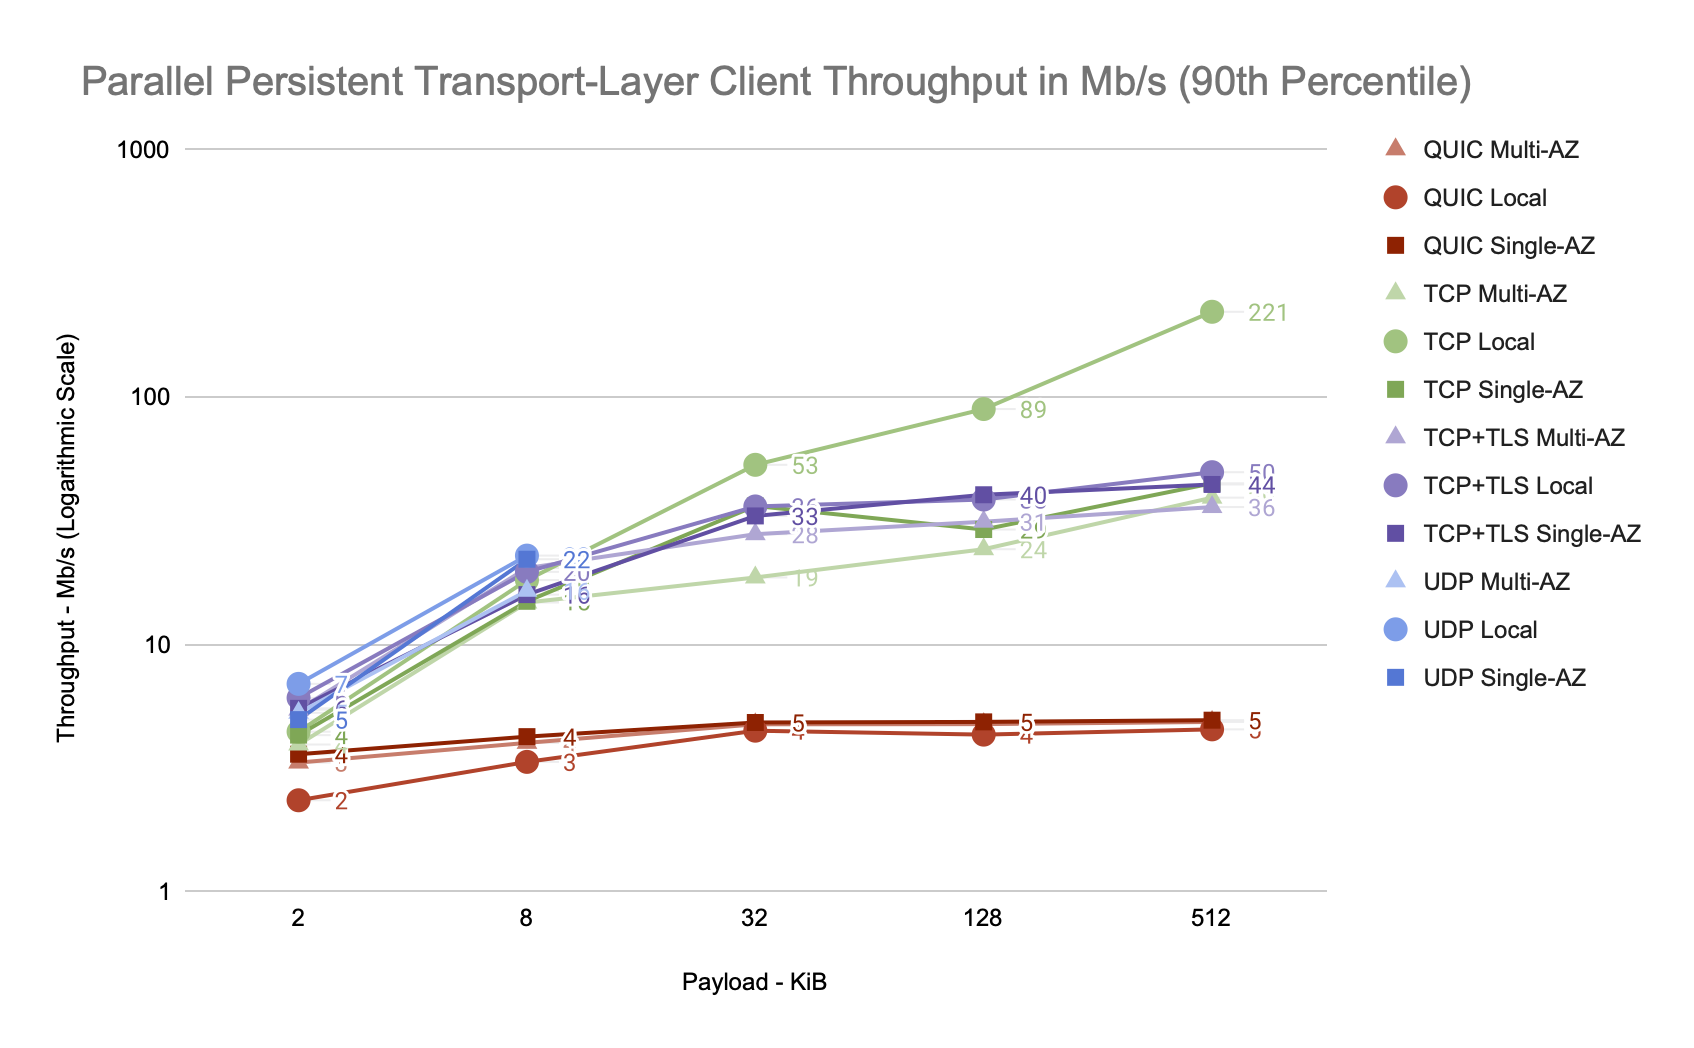
\includegraphics[width=\linewidth]{figures/charts/Parallel Persistent Transport-Layer Client Throughput in Mb_s (90th Percentile).png}
    \caption{Ephemeral Transport-Layer Client Throughput in Mb/s (90th Percentile)}
    \label{fig:parallel_transport_throughput}
\end{figure}

\clearpage

\subsubsection{CPU Usage}

Charts on Figures \ref{fig:sequential_client_app_cpu}, \ref{fig:parallel_client_app_cpu}, \ref{fig:sequential_server_app_cpu}, and \ref{fig:parallel_server_app_cpu} represent the \gls{cpu} usage of clients and servers during ephemeral and persistent experiments.

\subsubsection*{Overall Clients CPU Usage}

Application-layer protocols CPU Usage results behavior is similar to transport-layer's. Parallel requests with 32KiB and smaller payloads had a lower CPU usage when compared to sequential requests. And as requests payloads reaches 128KiB size, parallel requests CPU usage surpasses sequential requests.

\subsubsection*{HTTP/3's CPU Usage}

QUIC's CPU Usage (Figure \ref{fig:parallel_client_transport_cpu}) is almost the same as HTTP/3's (Figure \ref{fig:parallel_client_app_cpu}). As QUIC performs shift features that were usually implemented in the application-layer, it does most of the work necessary to manage traffic. Therefore, HTTP/3 is only an interface so applications can still use it as any other HTTP protocol.

\subsubsection*{Overall Server CPU Usage}

As other experiments, Server CPU usage remained roughly the same as client CPU usage. Client and servers still need to process the same amount of requests and responses, which explains why their CPU usage is so similar.

\clearpage

\begin{figure}[h!]
    \centering
    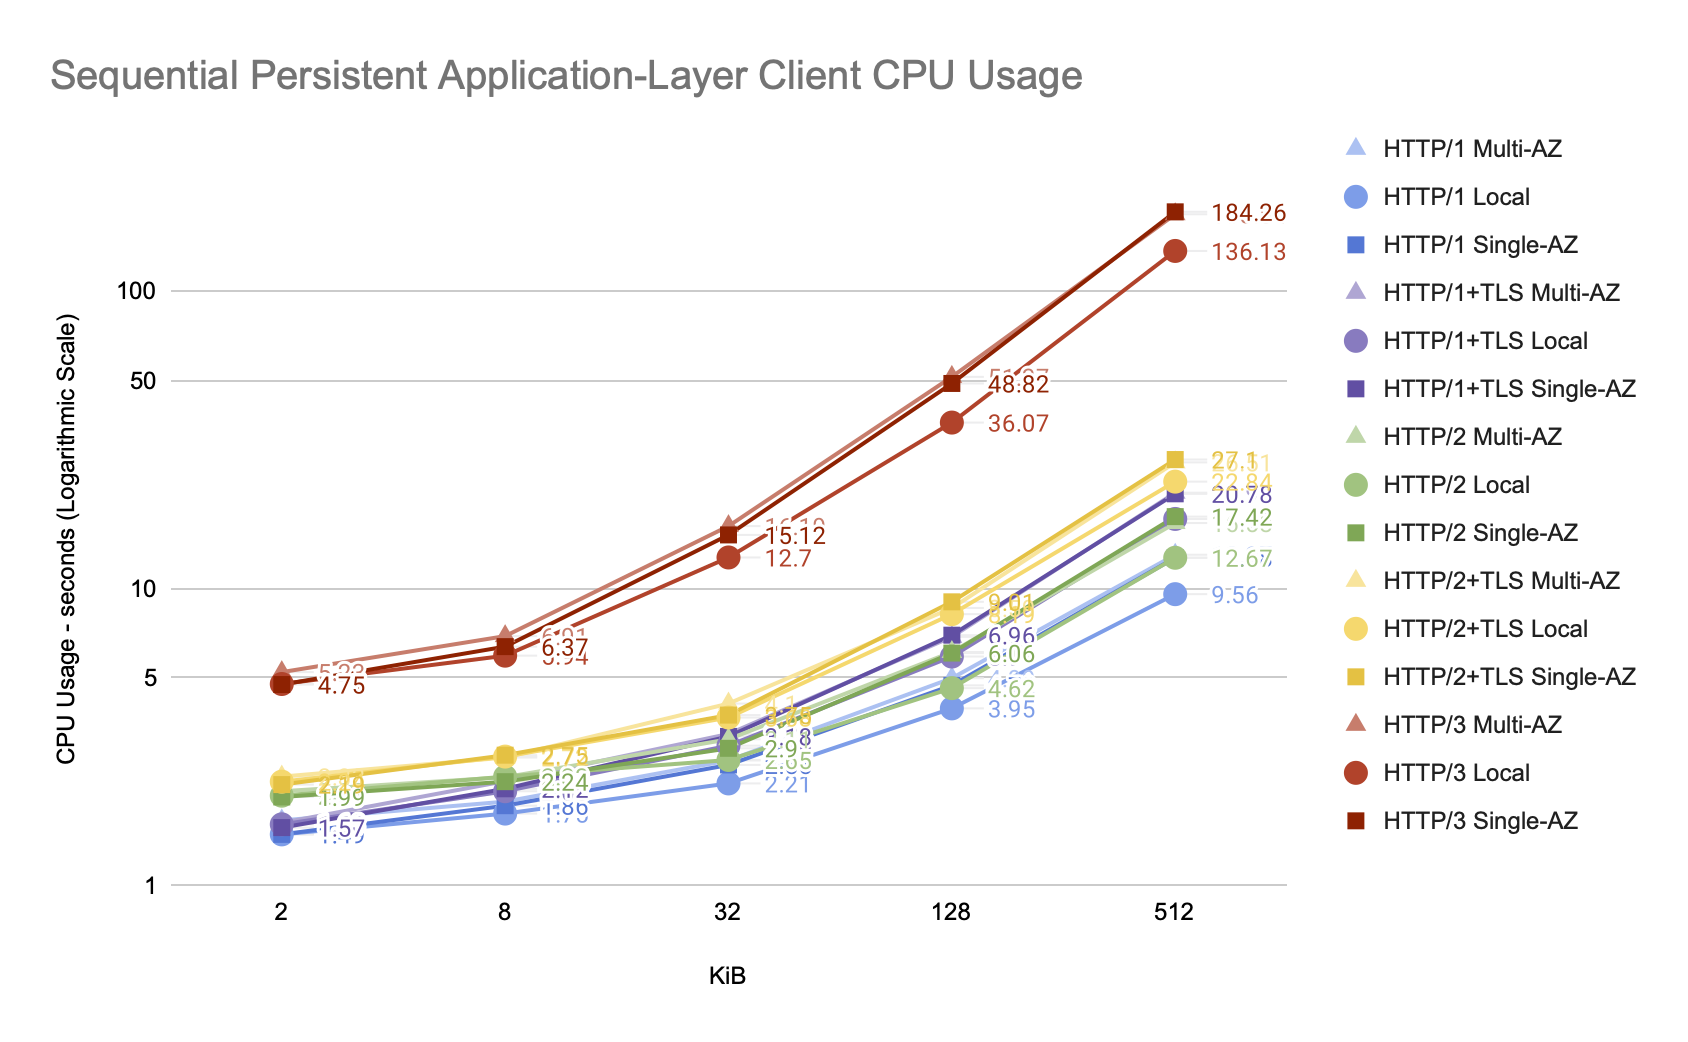
\includegraphics[width=\linewidth]{figures/charts/Sequential Persistent Application-Layer Client CPU Usage.png}
    \caption{Sequential Persistent Application-Layer Client CPU Usage}
    \label{fig:sequential_client_app_cpu}
\end{figure}
\begin{figure}[h!]
    \centering
    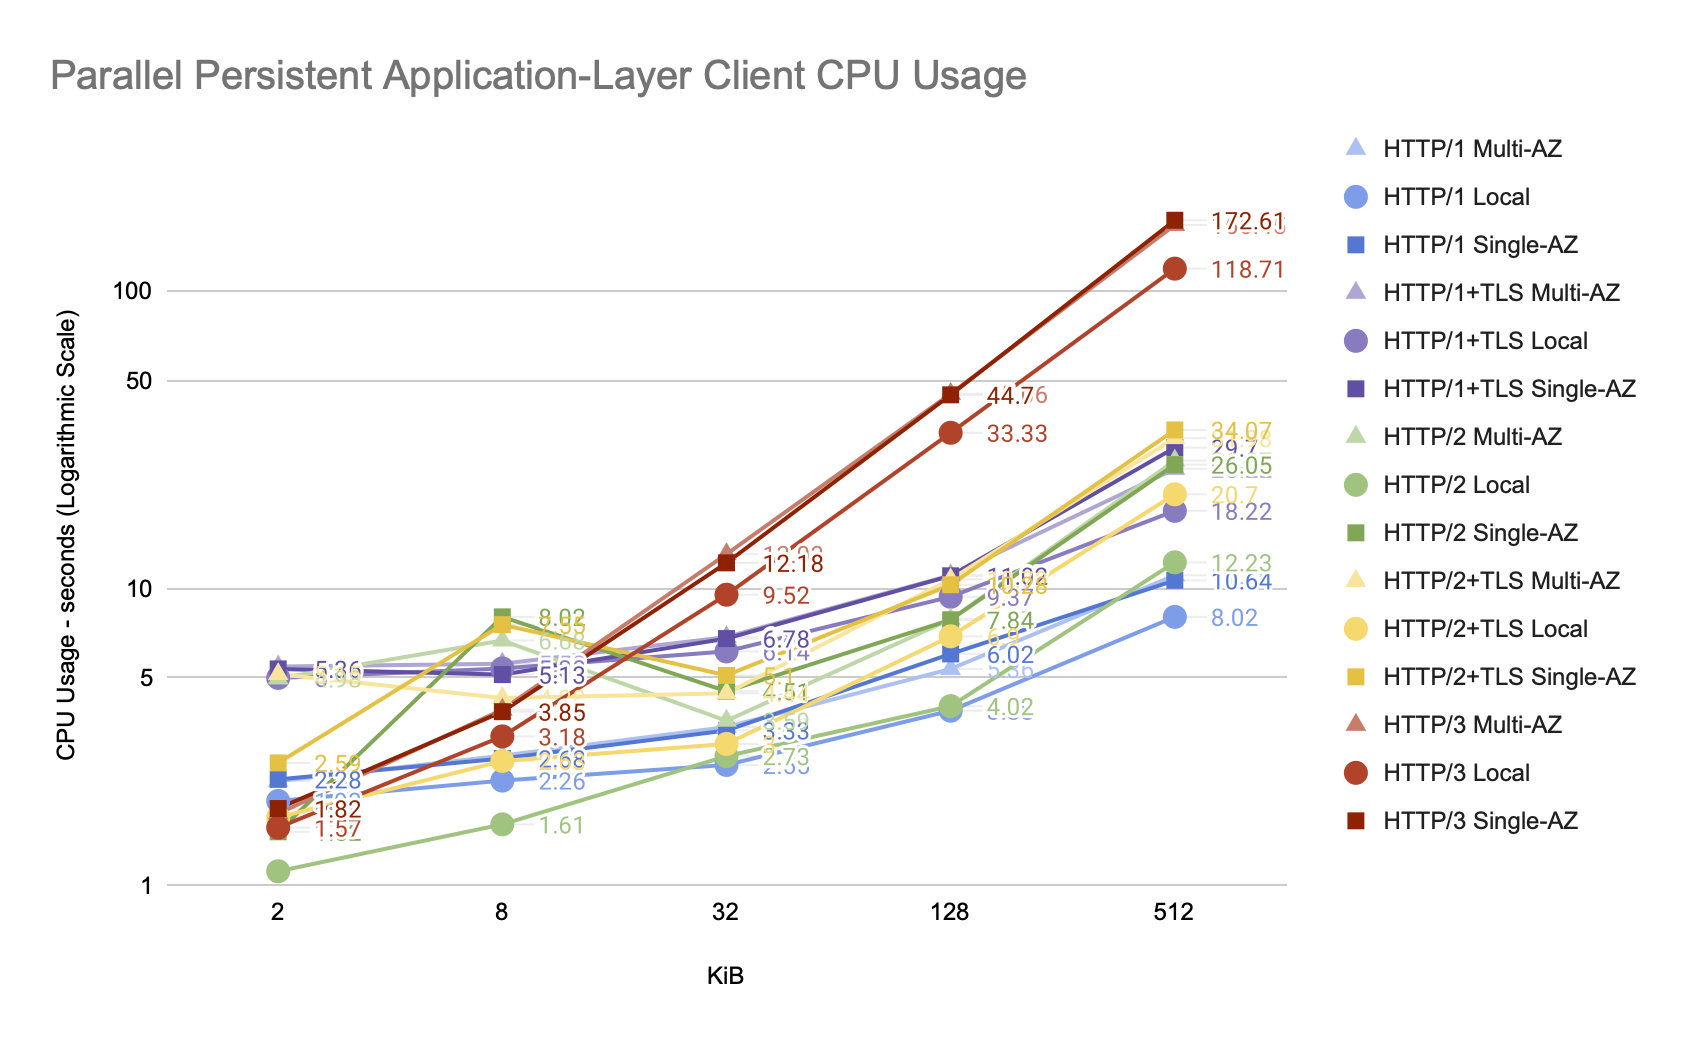
\includegraphics[width=\linewidth]{figures/charts/Parallel Persistent Application-Layer Client CPU Usage.png}
    \caption{Parallel Persistent Application-Layer Client CPU Usage}
    \label{fig:parallel_client_app_cpu}
\end{figure}

\begin{figure}[h!]
    \centering
    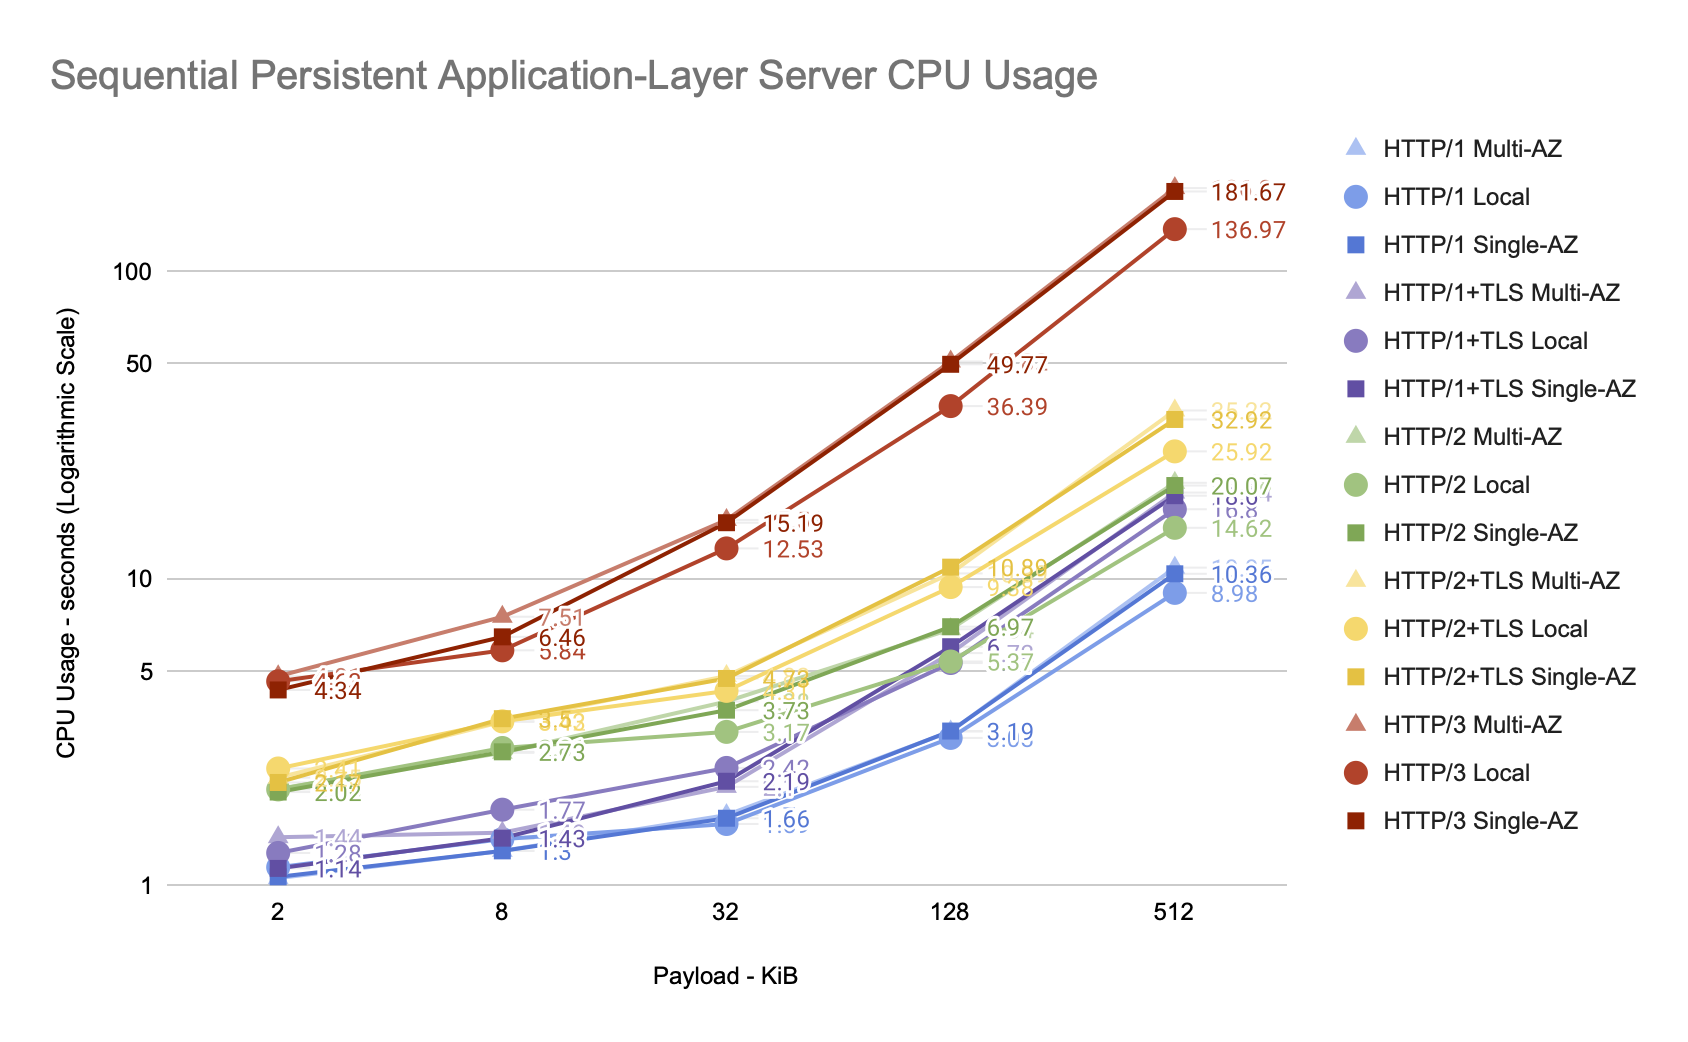
\includegraphics[width=\linewidth]{figures/charts/Sequential Persistent Application-Layer Server CPU Usage.png}
    \caption{Sequential Persistent Application-Layer Server CPU Usage}
    \label{fig:sequential_server_app_cpu}
\end{figure}
\begin{figure}[h!]
    \centering
    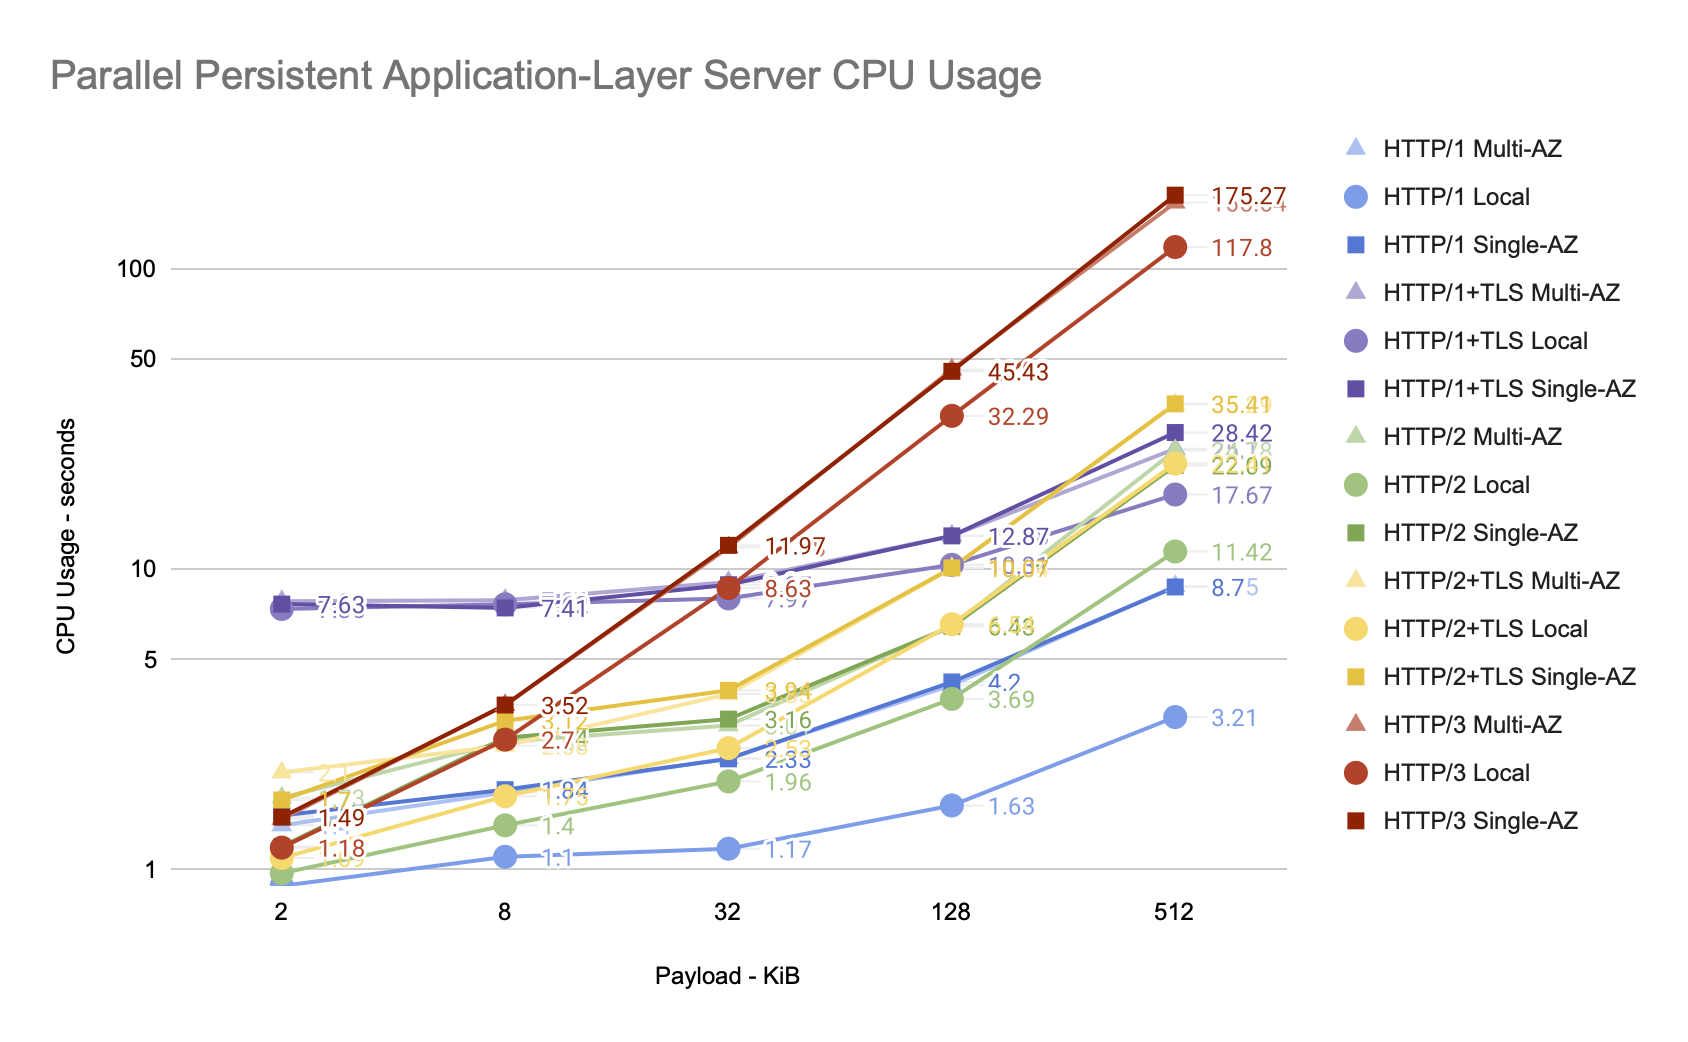
\includegraphics[width=\linewidth]{figures/charts/Parallel Persistent Application-Layer Server CPU Usage.png}
    \caption{Parallel Persistent Application-Layer Server CPU Usage}
    \label{fig:parallel_server_app_cpu}
\end{figure}

\clearpage

\subsection{Memory}

These charts represent the memory usage of clients and servers during ephemeral and persistent experiments.

These results were very similar to transport-layer experiments. \gls{http}/1 and \gls{http}/2 were the most memory efficient due to their simplicity and use of \gls{tcp} as transport protocol, which had similar results. \gls{http}/1+\gls{tls} and \gls{http}/2+\gls{tls} had increased memory usage due to \gls{tls} requirements for data encryption and \gls{tls} handshake. Finally, \gls{http}/3 had to use more memory due to QUIC’s overhead, which trades memory for efficiency.

During ephemeral experiments, Go’s garbage collector also had problems dealing with the high rate of created clients. Problem that begins worse with small data sizes, but it gets amortized as data sizes gets larger, which results in slower responses from the server, allowing Go’s garbage collector time to do its job.

\clearpage

\begin{figure}[h!]
    \centering
    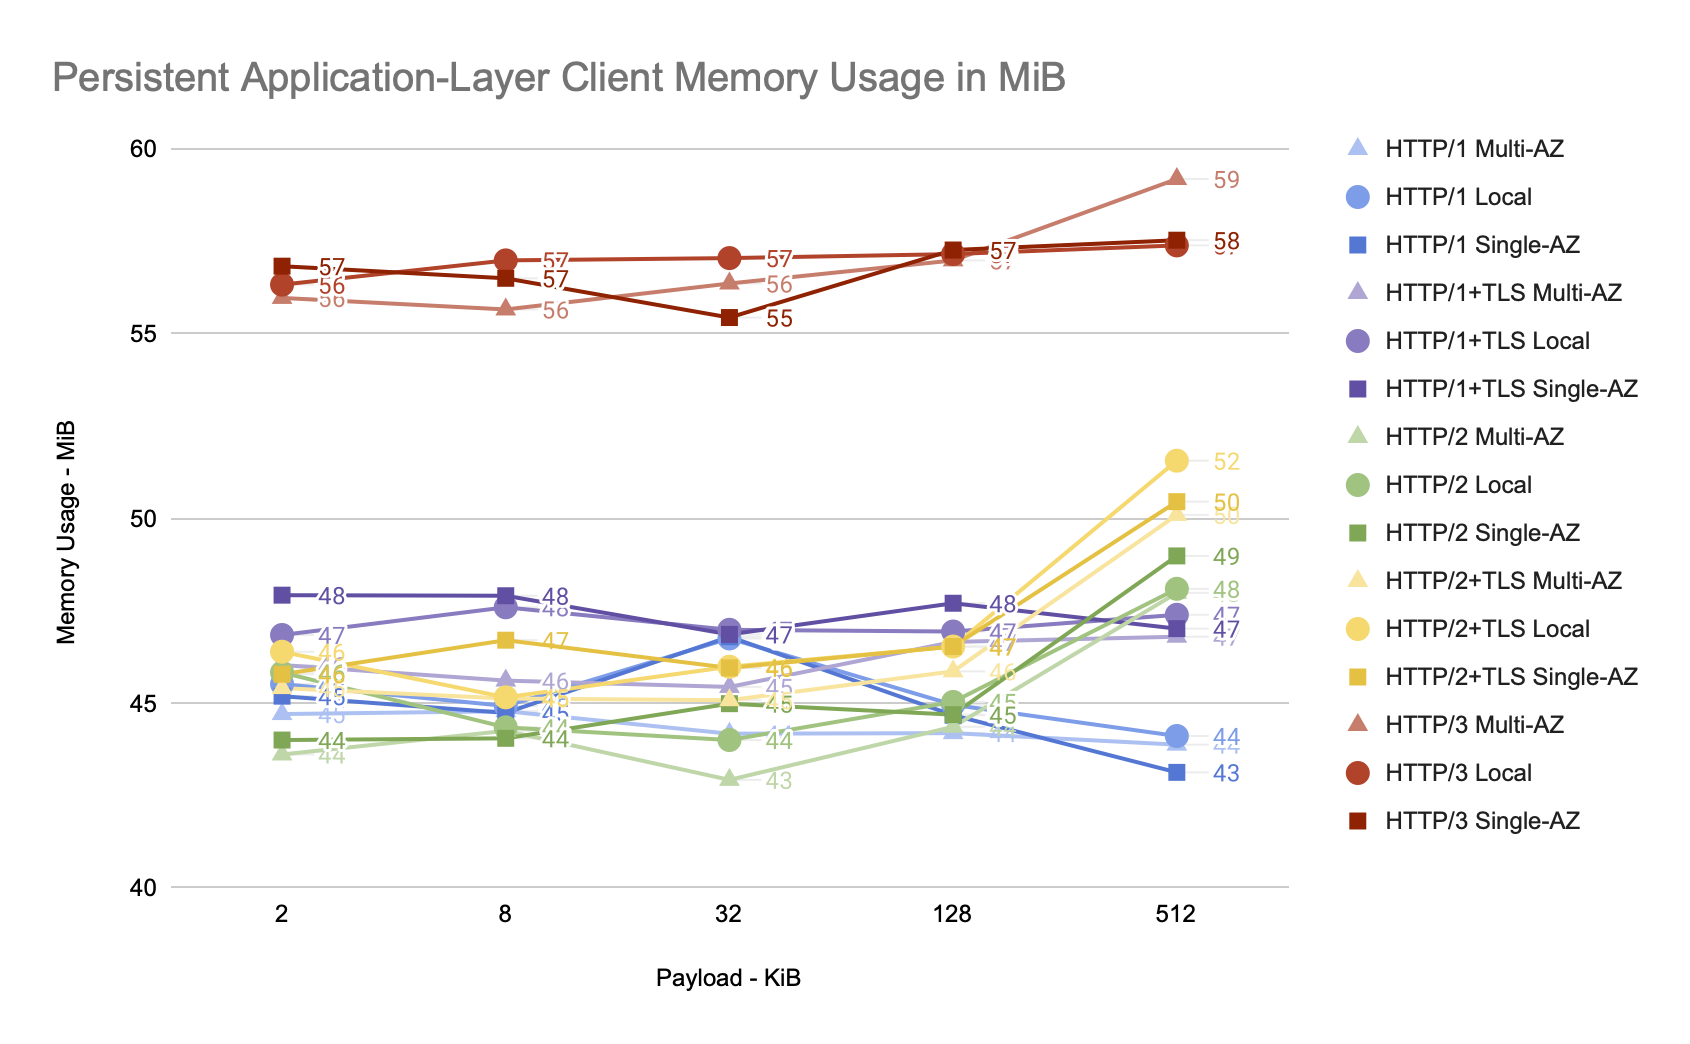
\includegraphics[width=\linewidth]{figures/charts/Persistent Application-Layer Client Memory Usage in MiB.png}
    \caption{Persistent Application-Layer Client Memory Usage in MiB}
    \label{fig:persistent_client_app_memory}
\end{figure}

\begin{figure}[h!]
    \centering
    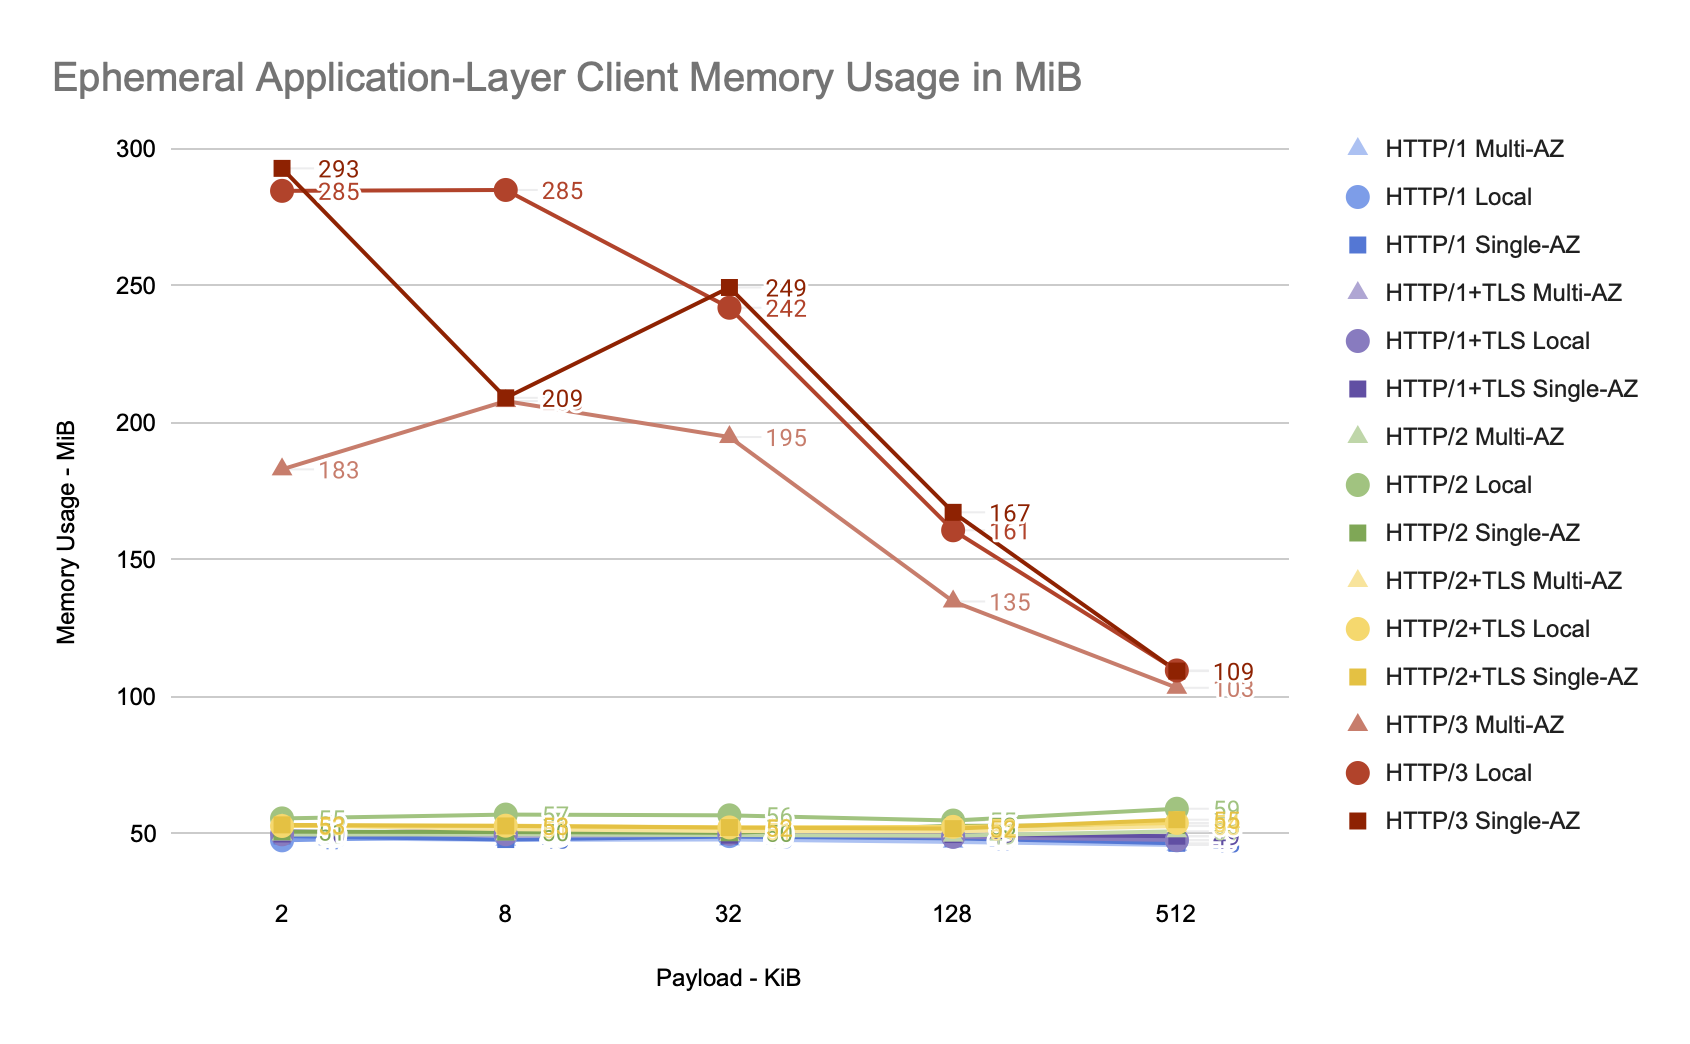
\includegraphics[width=\linewidth]{figures/charts/Ephemeral Application-Layer Client Memory Usage in MiB.png}
    \caption{Ephemeral Application-Layer Client Memory Usage in MiB}
    \label{fig:ephemeral_client_app_memory}
\end{figure}

\begin{figure}[h!]
    \centering
    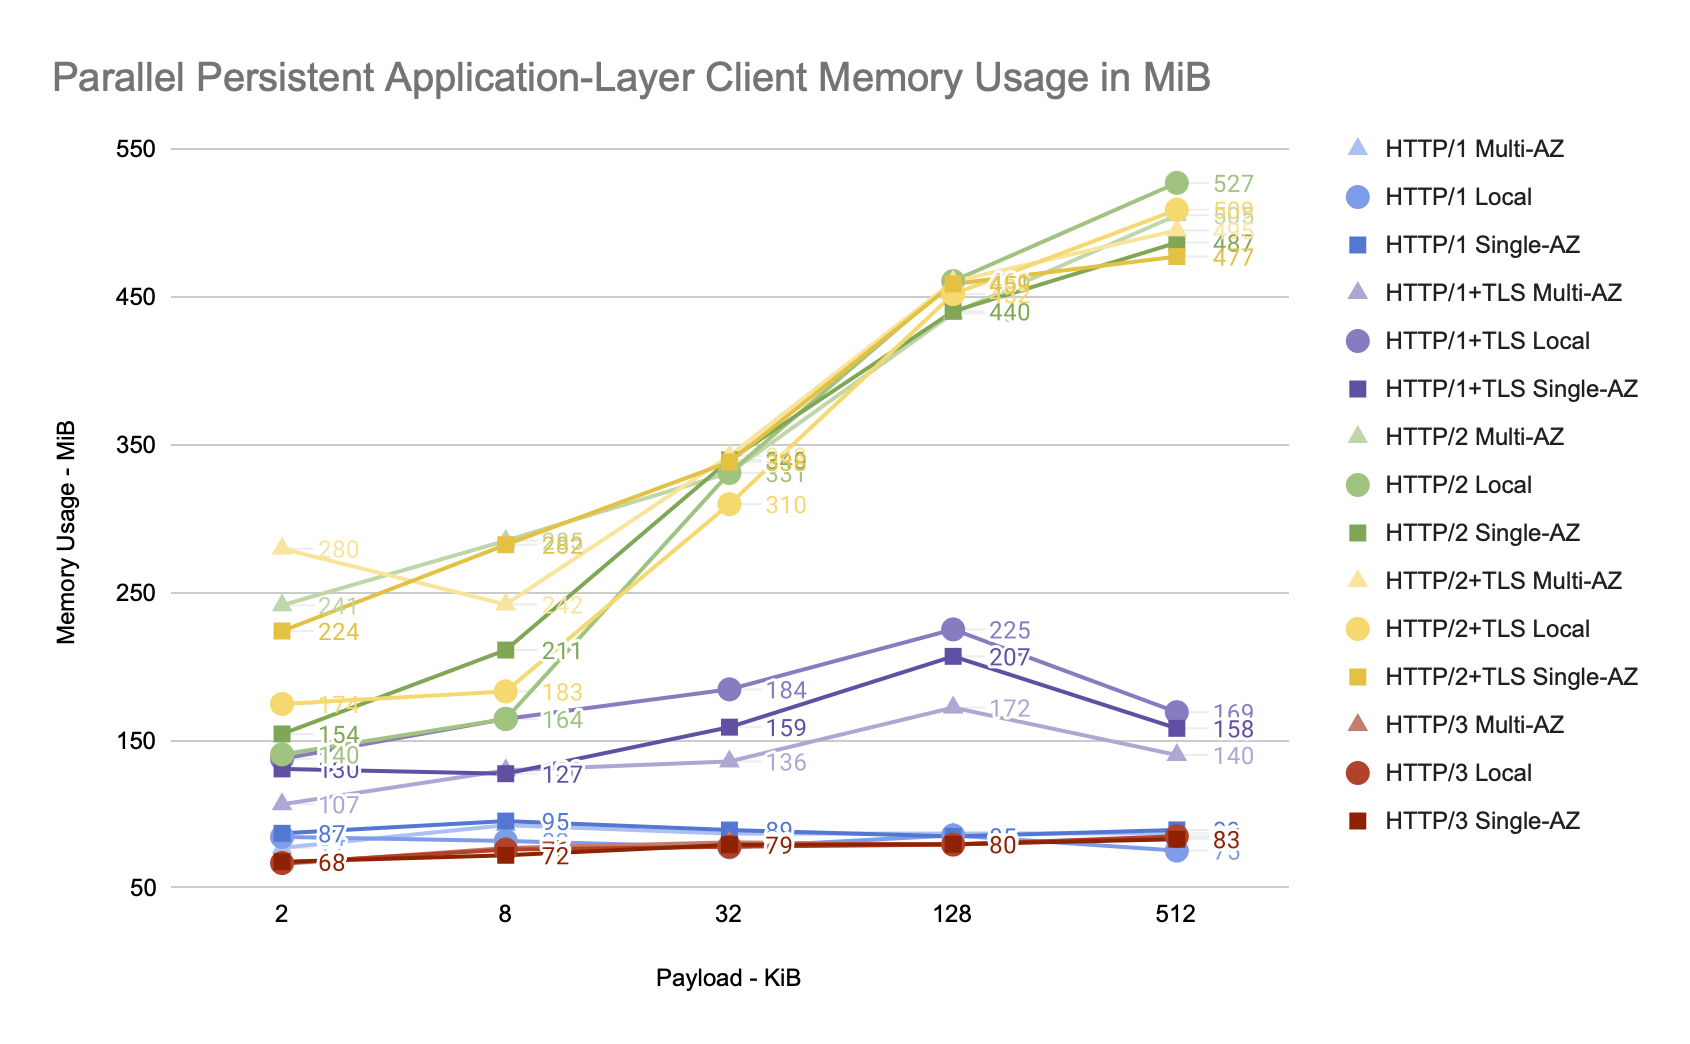
\includegraphics[width=\linewidth]{figures/charts/Parallel Persistent Application-Layer Client Memory Usage in MiB.png}
    \caption{Parallel Persistent Application-Layer Client Memory Usage in MiB}
    \label{fig:parallel_client_app_memory}
\end{figure}

\begin{figure}[h!]
    \centering
    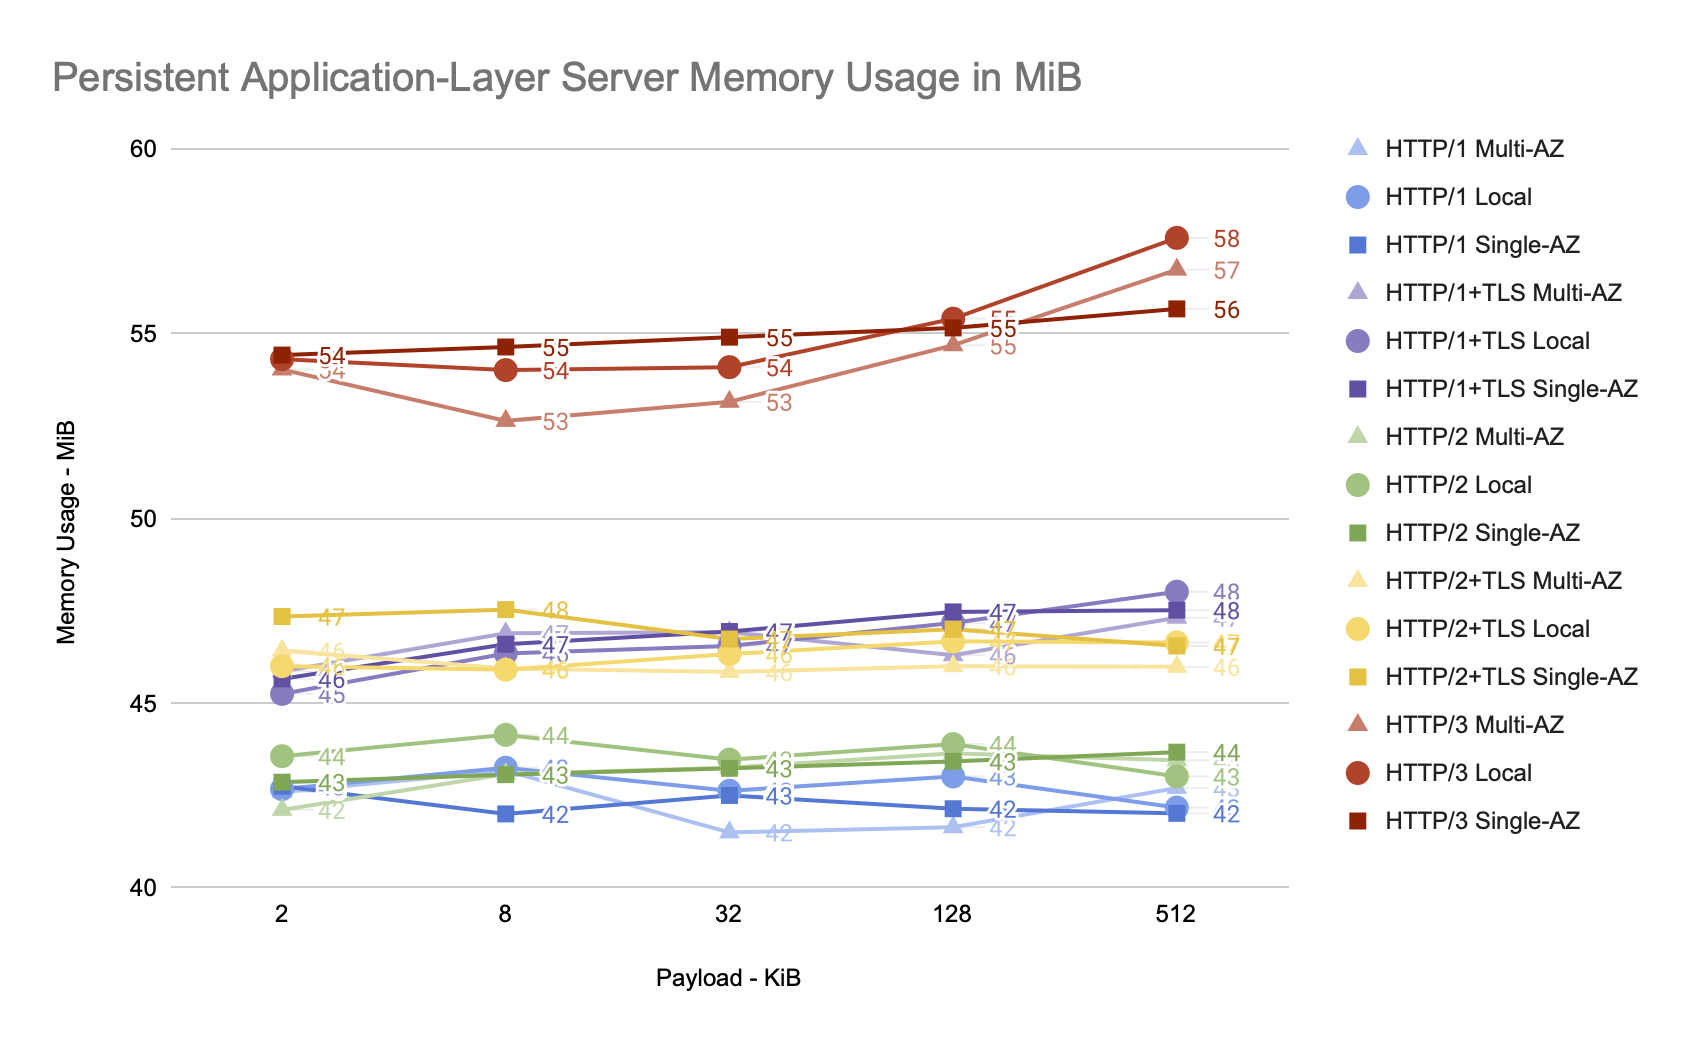
\includegraphics[width=\linewidth]{figures/charts/Persistent Application-Layer Server Memory Usage in MiB.png}
    \caption{Persistent Application-Layer Server Memory Usage in MiB}
    \label{fig:persistent_server_app_memory}
\end{figure}

\begin{figure}[h!]
    \centering
    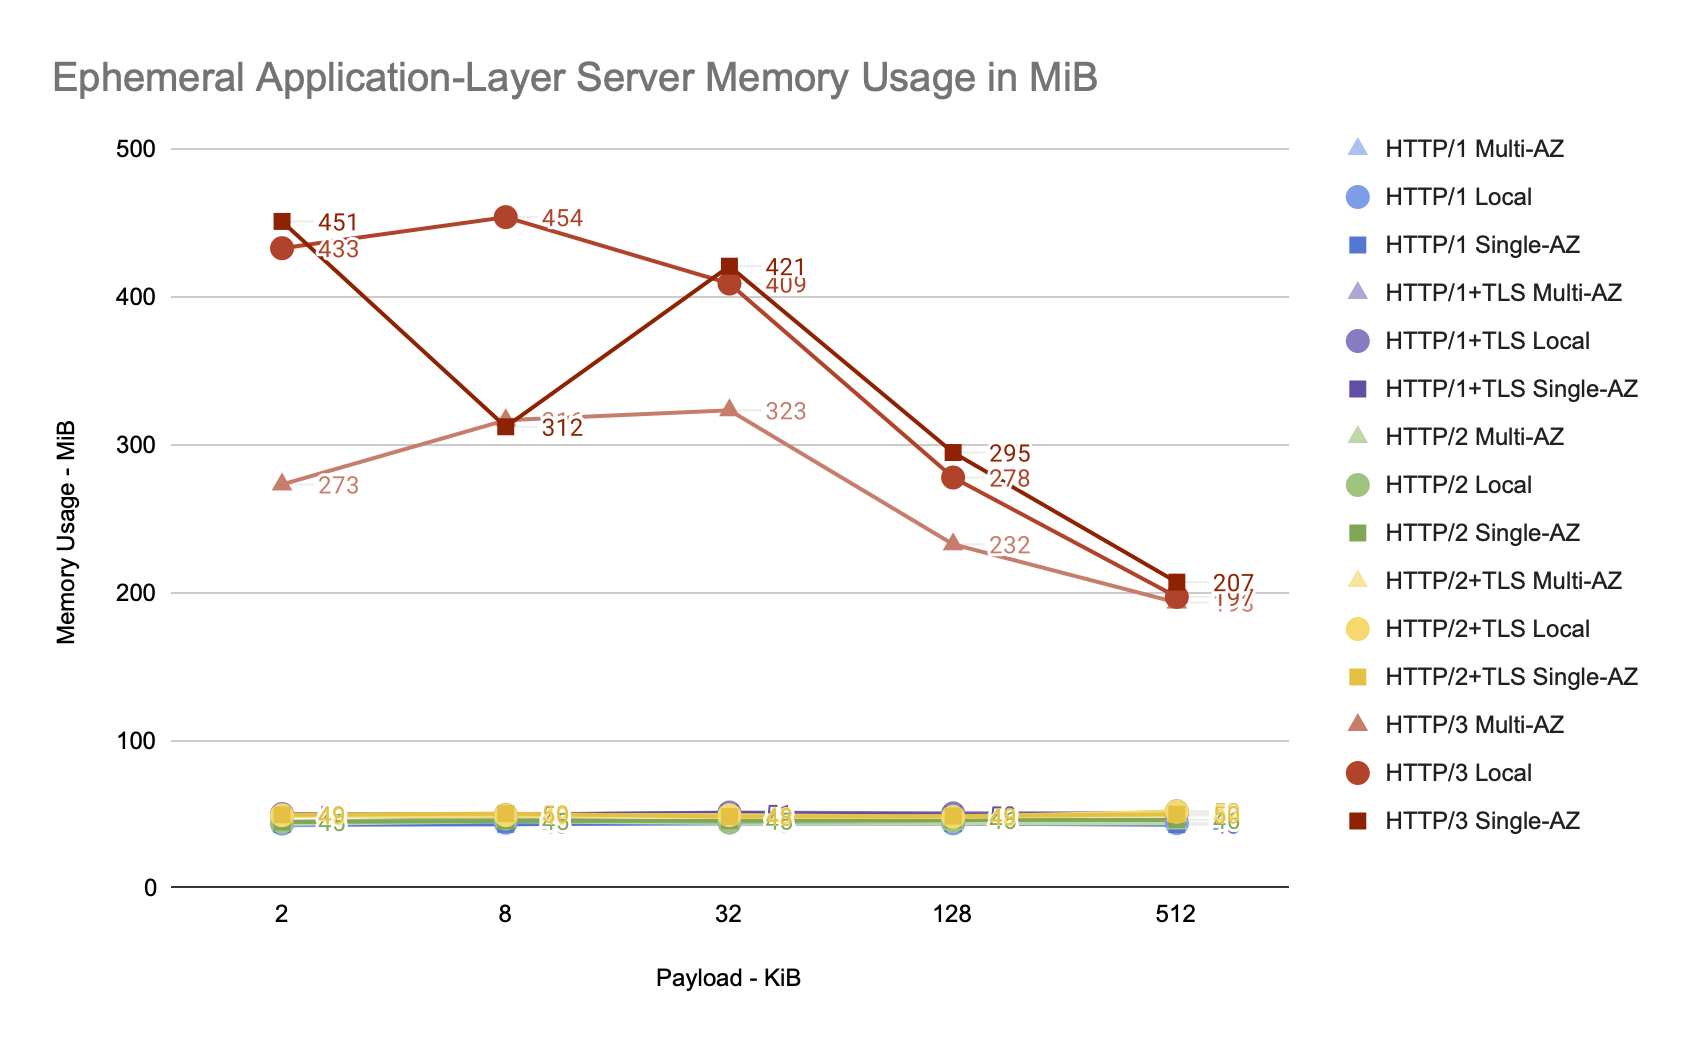
\includegraphics[width=\linewidth]{figures/charts/Ephemeral Application-Layer Server Memory Usage in MiB.png}
    \caption{Ephemeral Application-Layer Server Memory Usage in MiB}
    \label{fig:ephemeral_server_app_memory}
\end{figure}

\begin{figure}[h!]
    \centering
    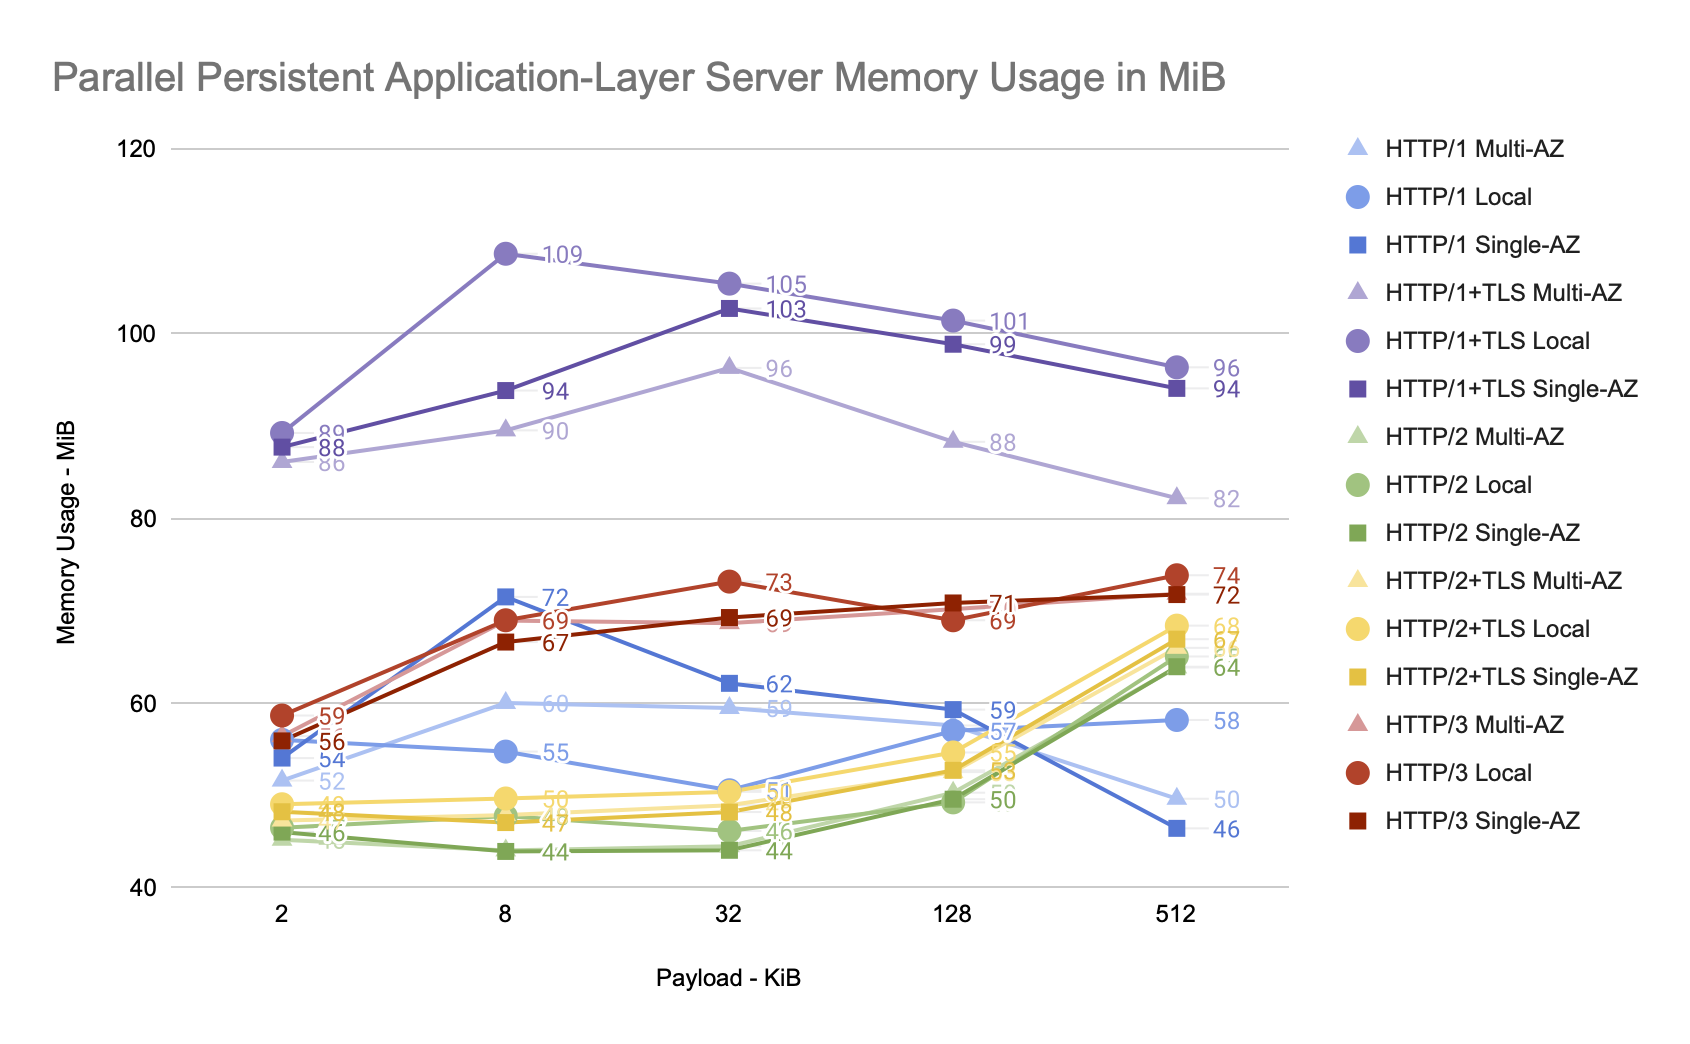
\includegraphics[width=\linewidth]{figures/charts/Parallel Persistent Application-Layer Server Memory Usage in MiB.png}
    \caption{Parallel Persistent Application-Layer Server Memory Usage in MiB}
    \label{fig:parallel_server_app_memory}
\end{figure}

\clearpage

\section{Cost}

<INSERT>

\clearpage

\subsection{Summary}

<INSERT>

\clearpage

\section{Application Protocols Experiments}

\clearpage

\subsection{Latency \& Throughput}

Charts on Figures \ref{fig:persistent_transport_latency}, \ref{fig:ephemeral_transport_latency}, \ref{fig:parallel_transport_latency}, \ref{fig:persistent_transport_throughput}, \ref{fig:ephemeral_transport_throughput}, \ref{fig:parallel_transport_throughput} represent the \gls{p90} of Latency and Throughput of all 10000 requests made by the persistent and ephemeral clients during the experiments.

Throughout these charts it is possible to observe an order pattern. Local experiments usually were more performatic when compared to Single-\gls{az} experiments. Additionally, the latter results were better than Multi-\gls{az} experiments due to the overhead from sending the datagram to another data center, even though remaining in the same region.

\gls{udp} Multi-\gls{az} and Single-\gls{az} experiments only succeeded on the first two iterations of each run when the data transferred was 2KiB and 8KiB. This was expected since pure \gls{udp} does not have any reliability and is expected to lose user datagrams along the way. As was stated before, no additional logic was added to \gls{udp} since this would interfere with the results because it would alter \gls{udp} natural behaviour.

Local \gls{tcp} experiment was by far the most efficient, with almost zero latency when connection was persistent, reaching approximately 19Gb/s of speed when transferring 512KiB of data per request. It outperformed \gls{udp}, that even though is considered faster due to its unreliability and connectionless characteristics, it only reached 2.8Gb/s in the same scenario. This happened because, while \gls{tcp} is stream oriented, which enables it to send a continuous stream of data with no overhead, \gls{udp} is message oriented.

Nonetheless, ephemeral clients demonstrated that establishing connections can have a significant impact on \gls{tcp}’s performance. Local \gls{tcp} latency went from 0.19ms to 1.79ms and throughput from 19Gb/s to 2.2Gb/s. Both results are still better than other \gls{tcp} and all \gls{tcp}+\gls{tls}’ experiments \gls{p90}, but brings them to a similar level.

It is possible to observe \gls{tls} encryption overhead on \gls{tcp} during persistent clients experiments. Furthermore, during ephemeral clients this overhead increases due to having to perform a \gls{tls} handshake before every request.

QUIC’s experiments were the worst, with almost 7 times slower than \gls{tcp}+\gls{tls}’ Multi-\gls{az} experiment (with persistent client) latency and throughput. This demonstrates \gls{tcp}+\gls{tls} performs better than QUIC on a reliable network, with a low packet loss rate. However, QUIC performs better than \gls{tcp}+\gls{tls} on an unreliable network.

QUIC’s specifically designed to be used in environments such as a wireless network or a mobile device, both which have a high tendency to lose packets, and to break \gls{tcp} connections. QUIC solves these problems by implementing a more efficient way to deal with retransmission of lost packets, improving its throughput, and having a 0-\gls{rtt} handshake, which deals with broken connections by removing the need to perform a \gls{tcp} and \gls{tls} handshake.

Consequently, QUIC’s results show it's not meant to be used on distributed systems. These environments are usually part of a reliable network, meaning that \gls{tcp} is usually a better fit.

\subsection{Parallel}

All previous experiments performed requests sequentially, undermining the possible gain in efficiency of protocols that contain improvements to concurrent requests. Therefore this experiment tries to explore this scenario by performing all 10000 requests with 100 Goroutines, each performing 100 requests.

However, when packet size is the same, we fallback to a scenario where multiplexing is useless since any request performed in sequence is going to take more than the previous to complete. Therefore, this is similar to a pipelining scenario, where the requests finish in the order they were made.

\begin{figure}[h]
    \centering
    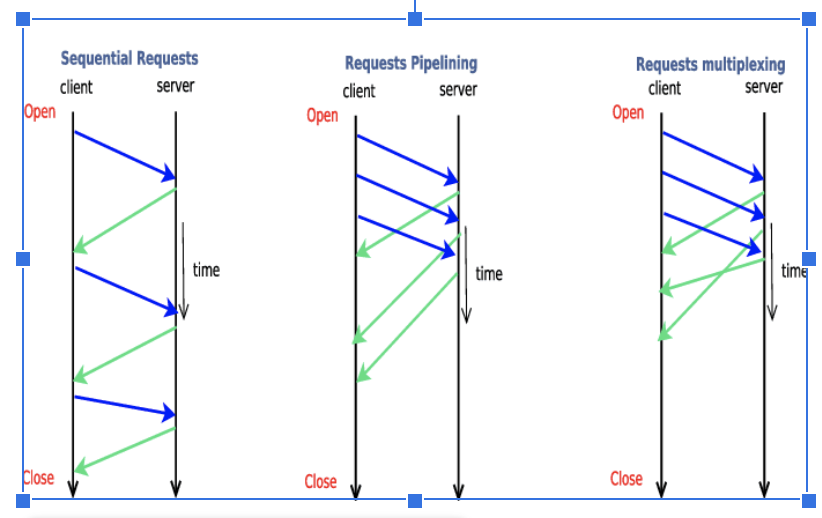
\includegraphics[width=\linewidth]{figures/pipelining.png}
    \caption{Pipelining}
    \label{fig:pipelining}
\end{figure}

\clearpage

\begin{figure}[h!]
    \centering
    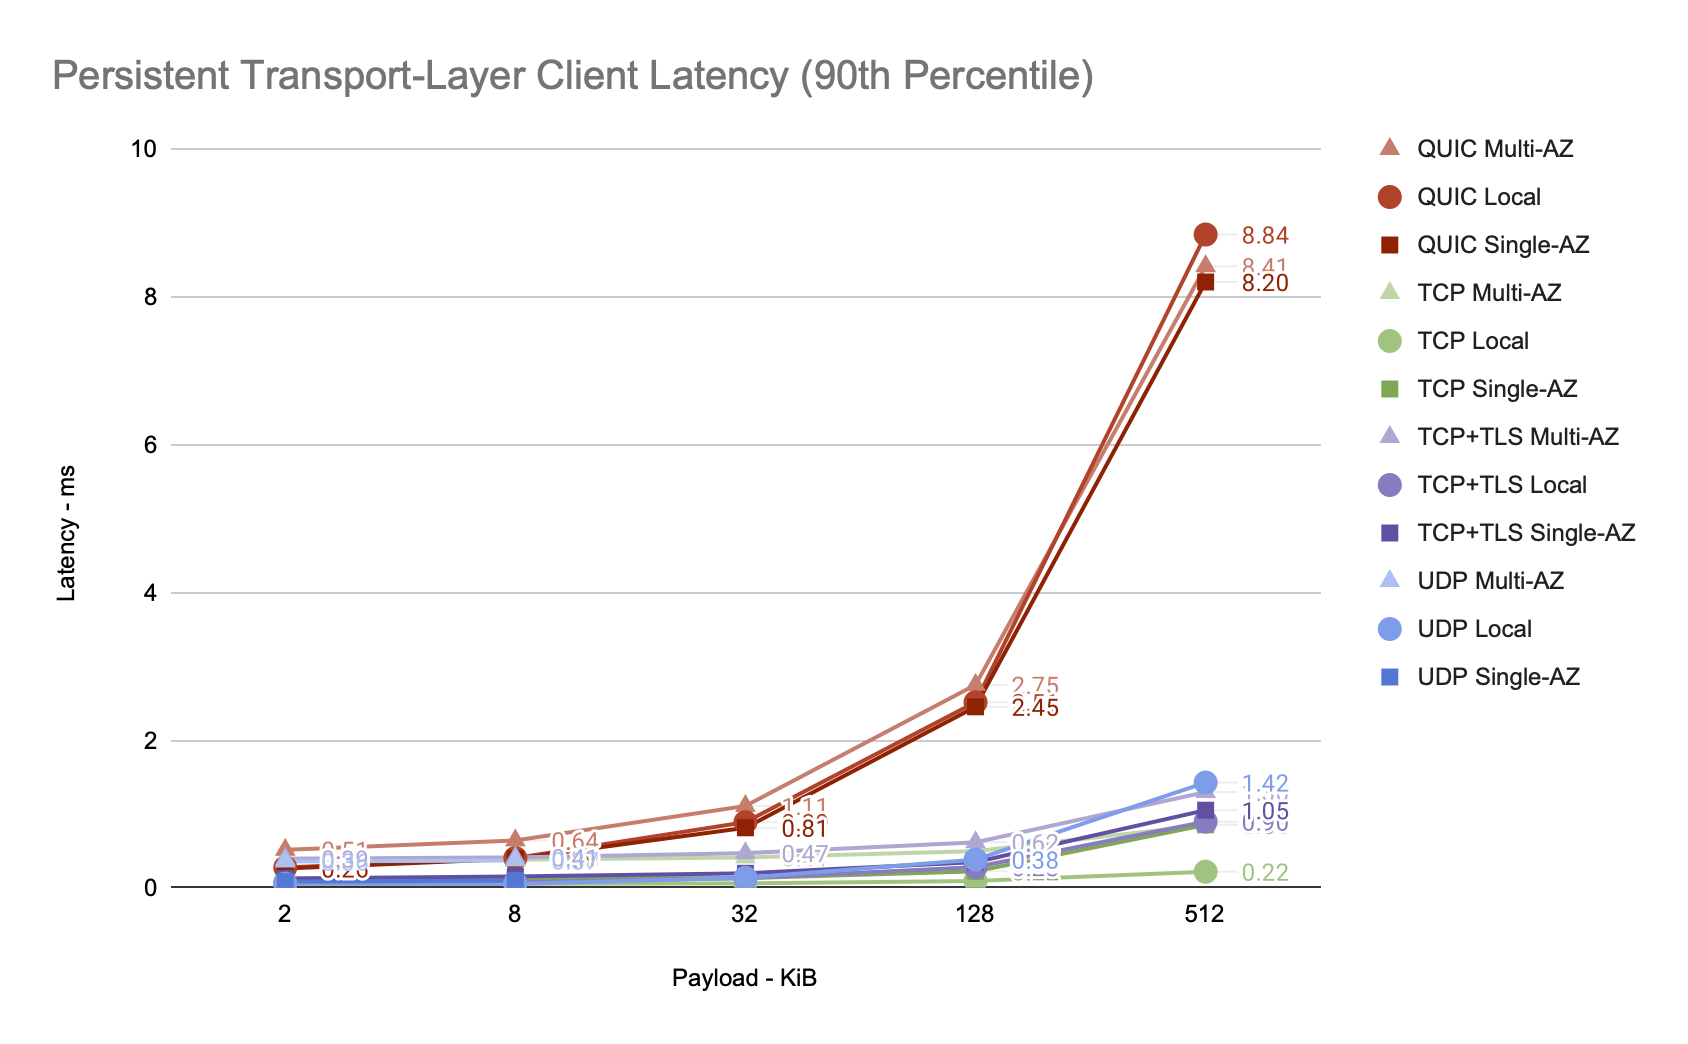
\includegraphics[width=\linewidth]{figures/charts/Persistent Transport-Layer Client Latency (90th Percentile).png}
    \caption{Persistent Transport-Layer Client Latency (90th Percentile)}
    \label{fig:persistent_transport_latency}
\end{figure}

\begin{figure}[h!]
    \centering
    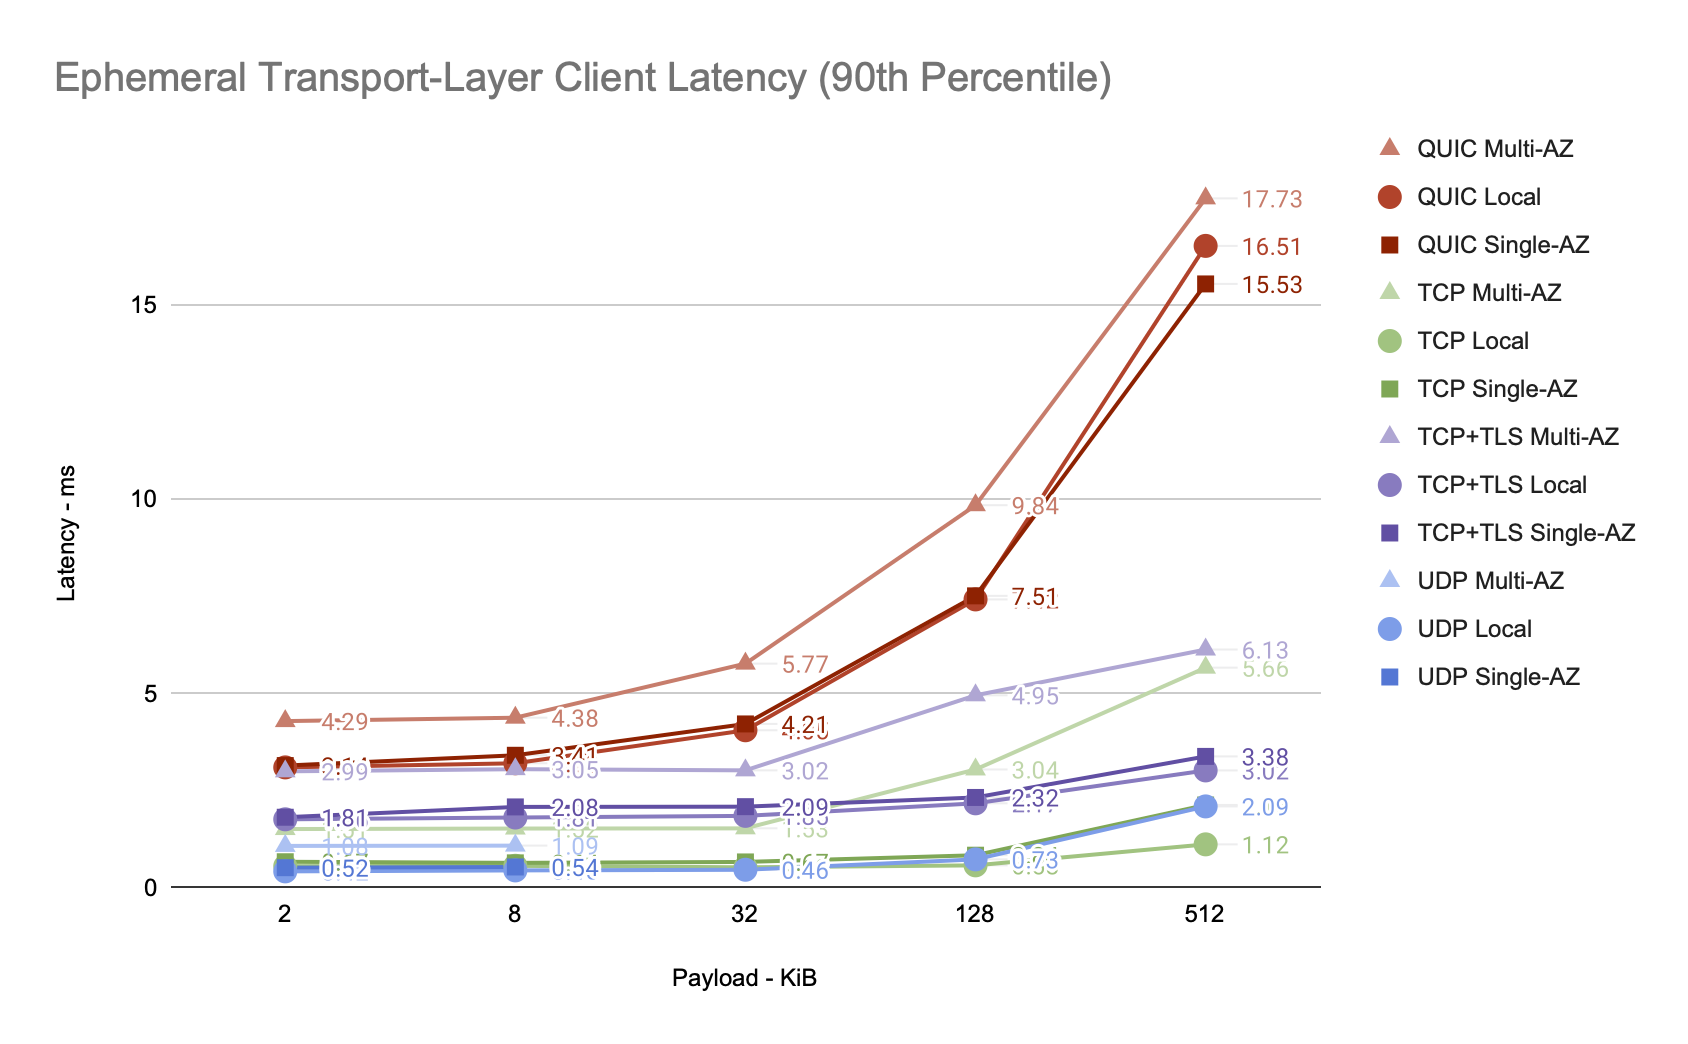
\includegraphics[width=\linewidth]{figures/charts/Ephemeral Transport-Layer Client Latency (90th Percentile).png}
    \caption{Ephemeral Transport-Layer Client Latency (90th Percentile)}
    \label{fig:ephemeral_transport_latency}
\end{figure}

\begin{figure}[h!]
    \centering
    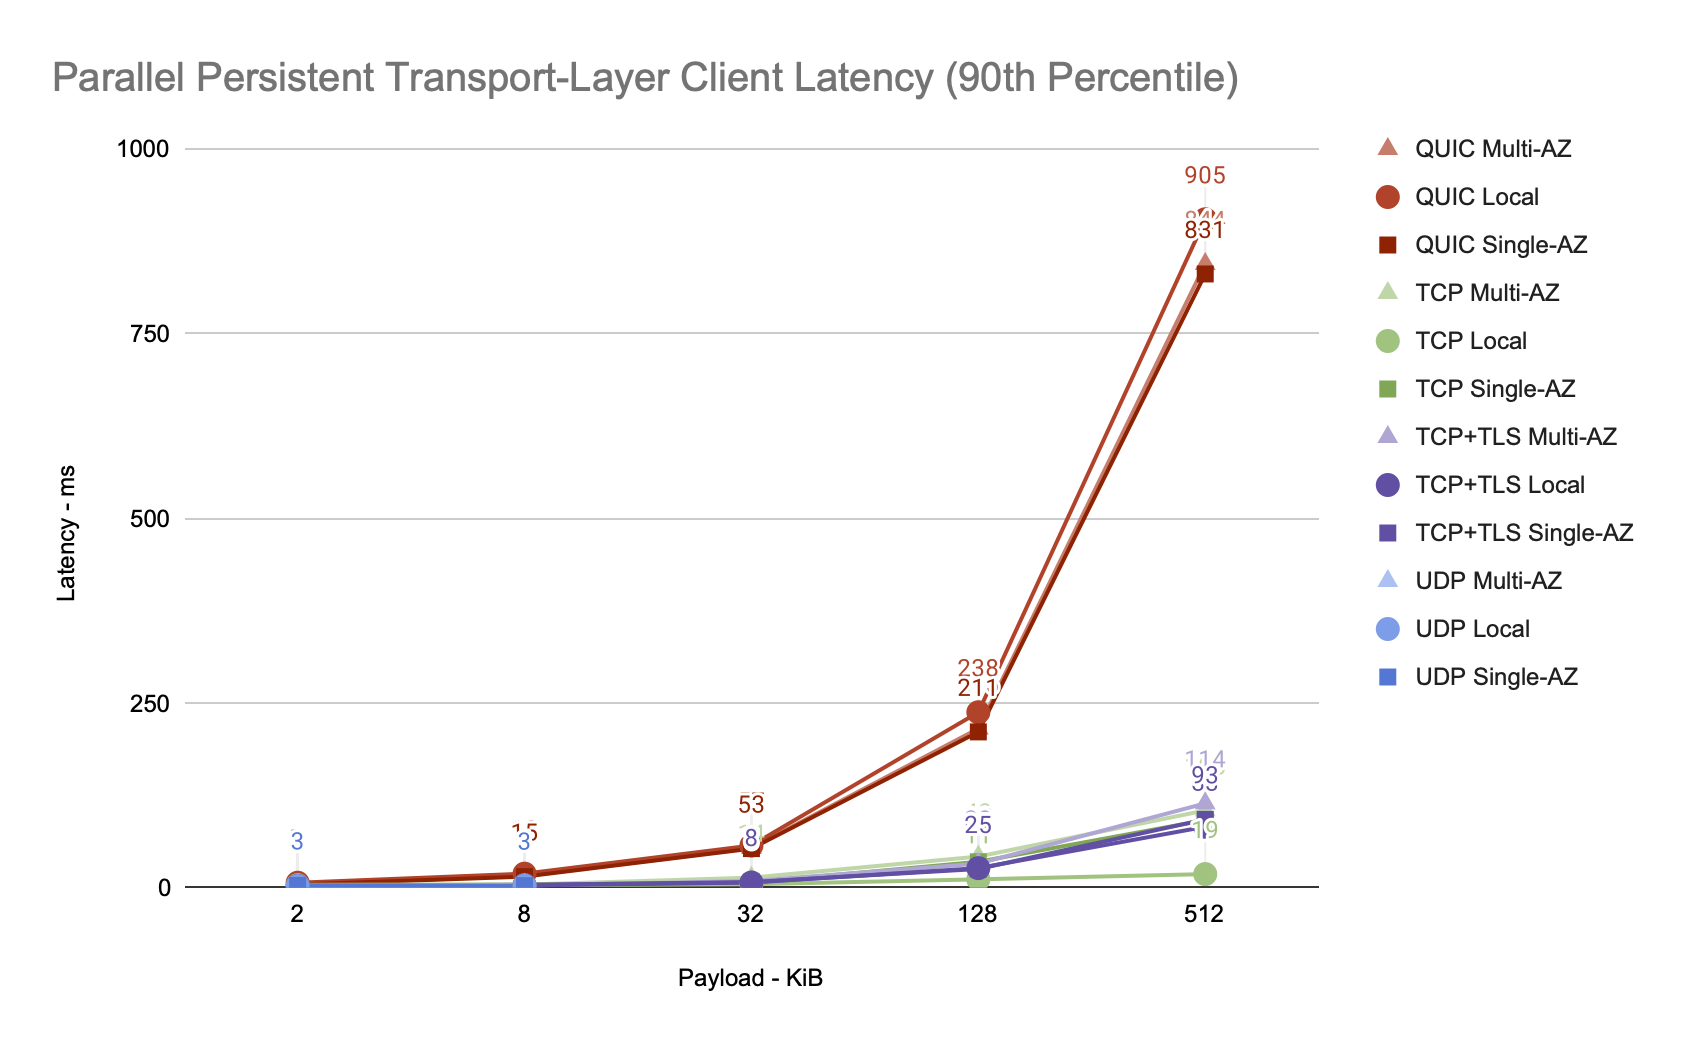
\includegraphics[width=\linewidth]{figures/charts/Parallel Persistent Transport-Layer Client Latency (90th Percentile).png}
    \caption{Parallel Persistent Transport-Layer Client Latency (90th Percentile)}
    \label{fig:parallel_transport_latency}
\end{figure}

\begin{figure}[h!]
    \centering
    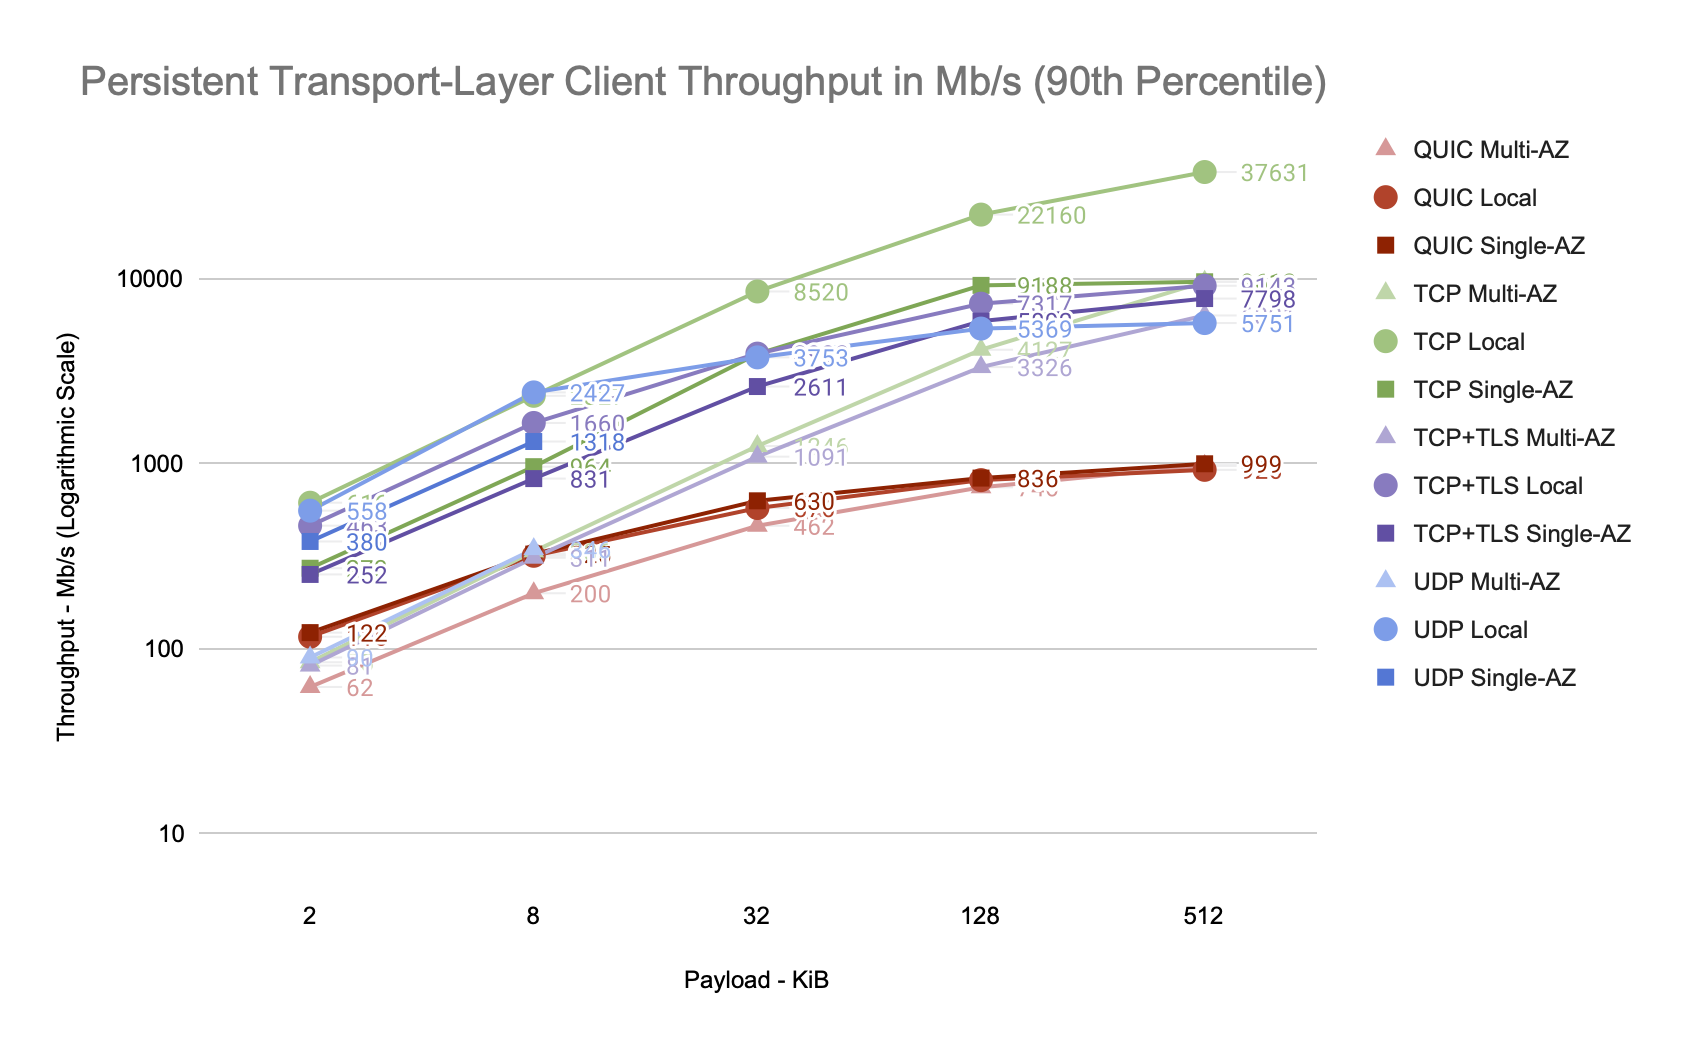
\includegraphics[width=\linewidth]{figures/charts/Persistent Transport-Layer Client Throughput in Mb_s (90th Percentile).png}
    \caption{Persistent Transport-Layer Client Throughput in Mb/s (90th Percentile)}
    \label{fig:persistent_transport_throughput}
\end{figure}

\begin{figure}[h!]
    \centering
    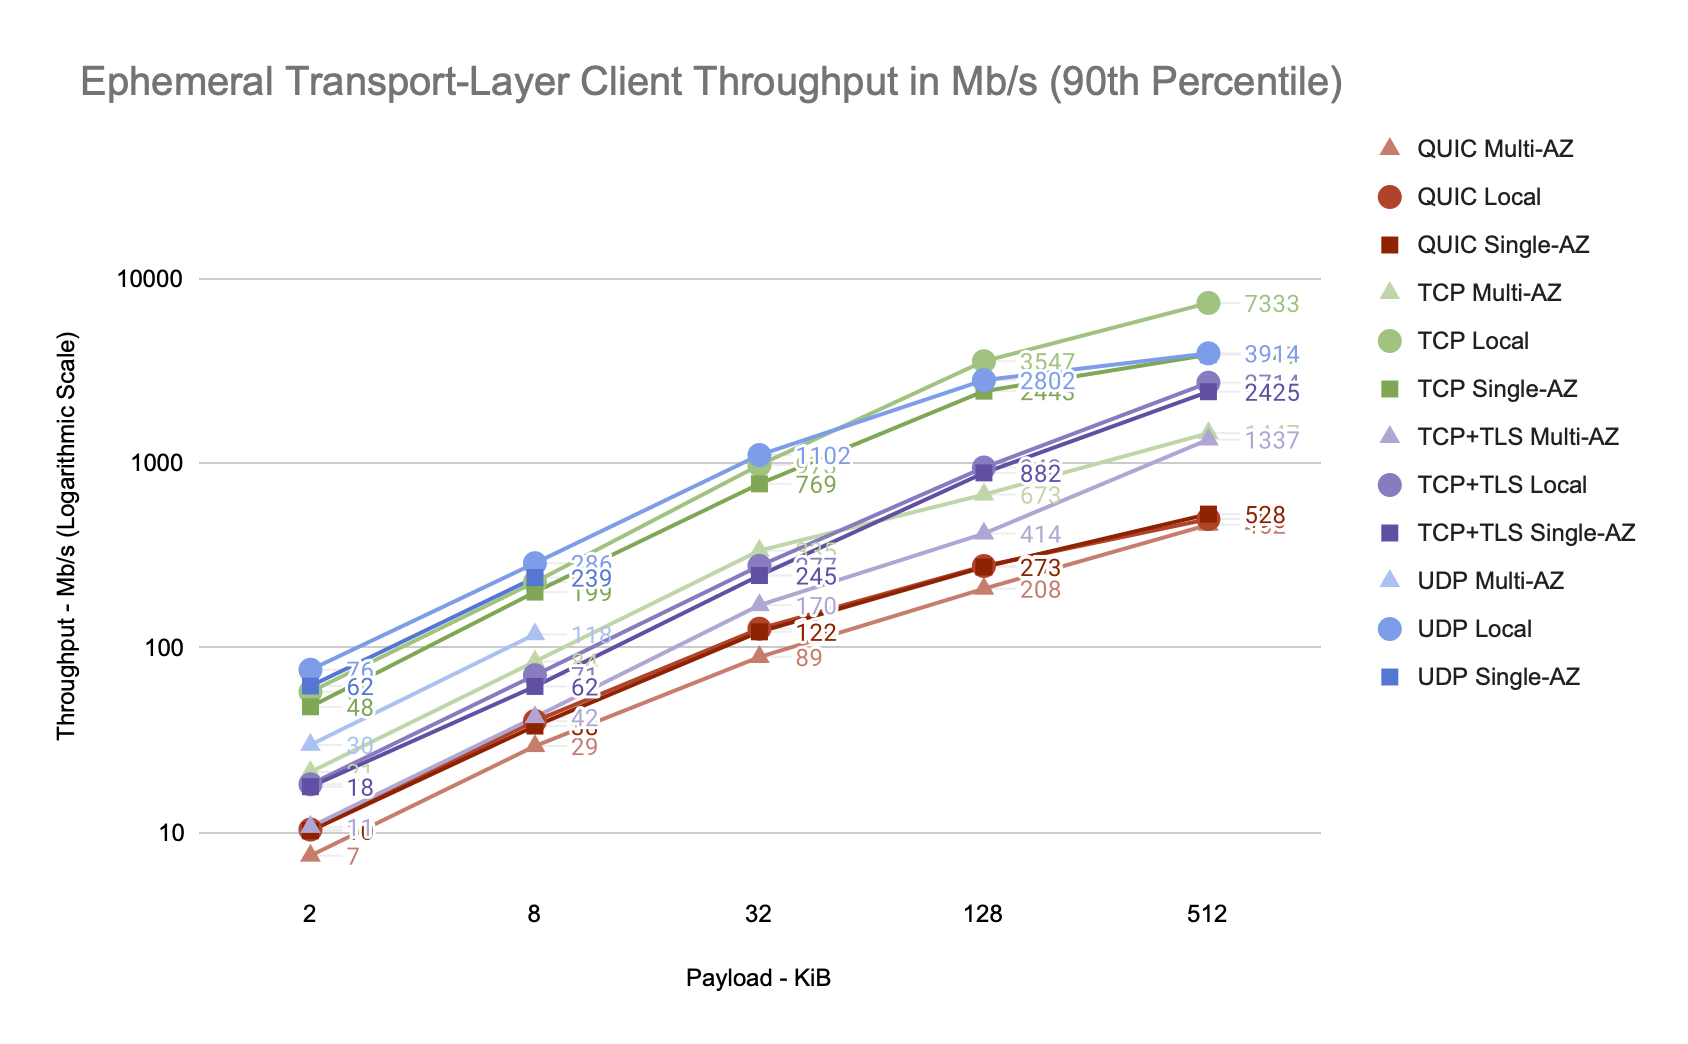
\includegraphics[width=\linewidth]{figures/charts/Ephemeral Transport-Layer Client Throughput in Mb_s (90th Percentile).png}
    \caption{Ephemeral Transport-Layer Client Throughput in Mb/s (90th Percentile)}
    \label{fig:ephemeral_transport_throughput}
\end{figure}

\begin{figure}[h!]
    \centering
    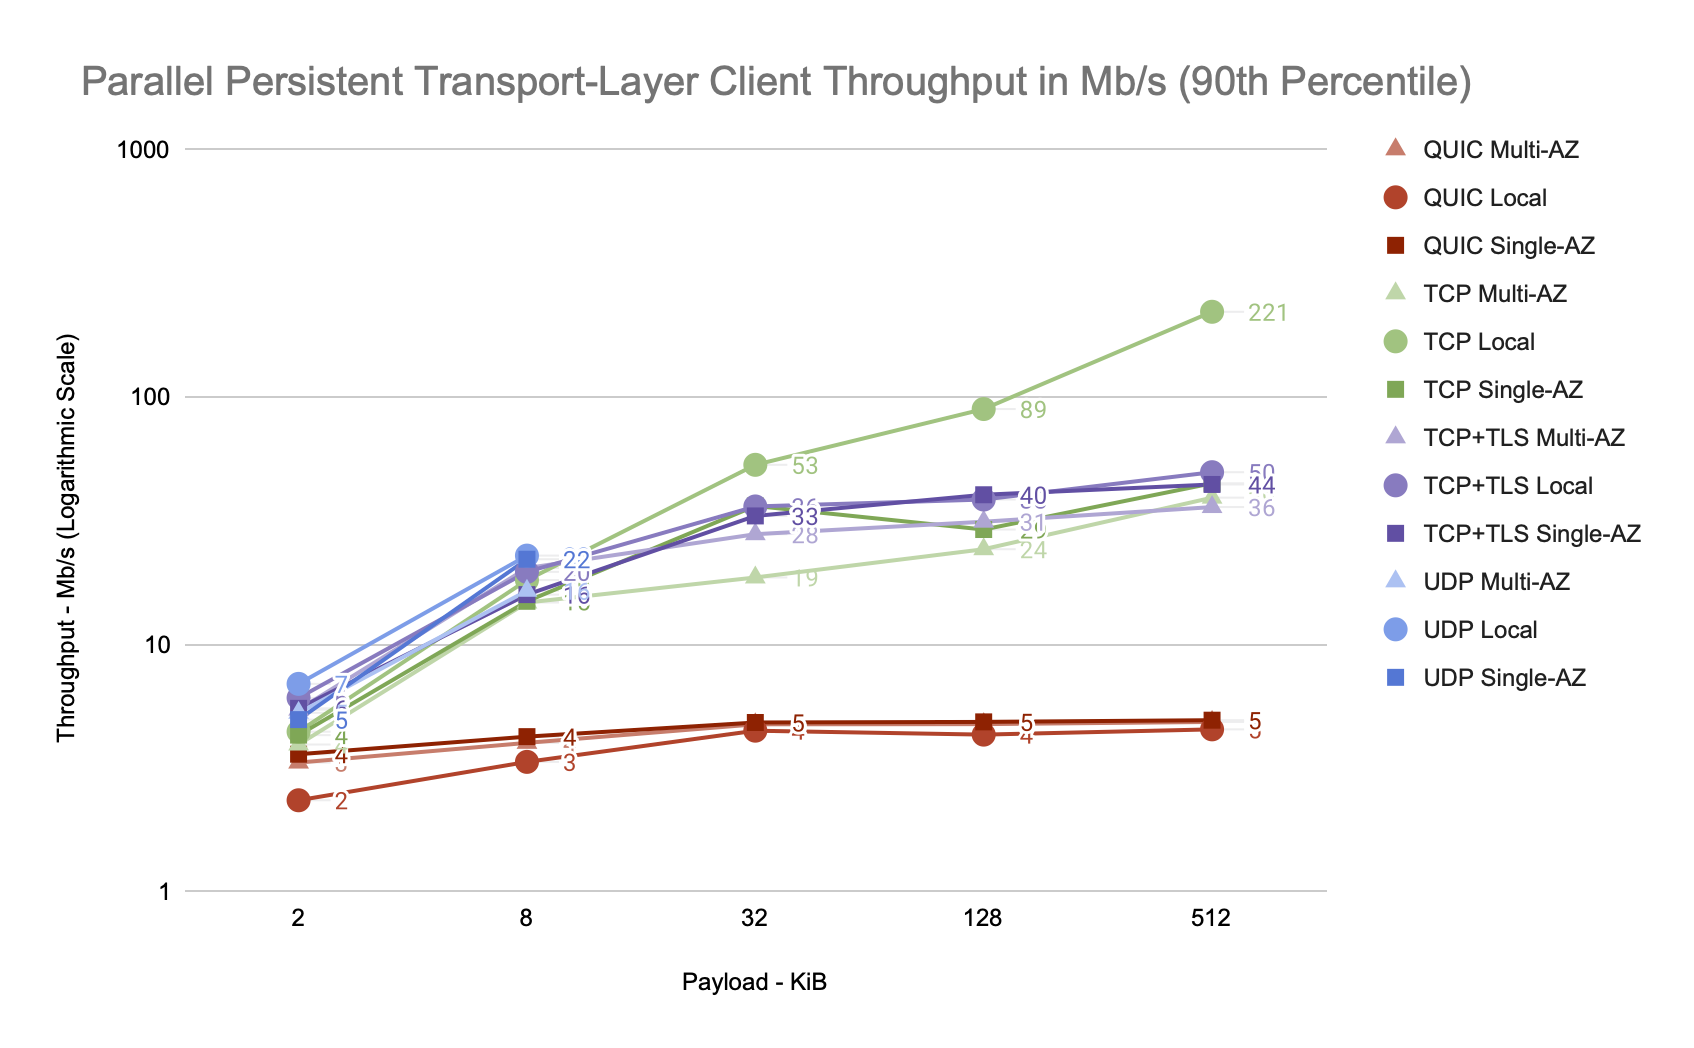
\includegraphics[width=\linewidth]{figures/charts/Parallel Persistent Transport-Layer Client Throughput in Mb_s (90th Percentile).png}
    \caption{Ephemeral Transport-Layer Client Throughput in Mb/s (90th Percentile)}
    \label{fig:parallel_transport_throughput}
\end{figure}

\clearpage

\subsubsection{CPU Usage}

Charts on Figures \ref{fig:sequential_client_app_cpu}, \ref{fig:parallel_client_app_cpu}, \ref{fig:sequential_server_app_cpu}, and \ref{fig:parallel_server_app_cpu} represent the \gls{cpu} usage of clients and servers during ephemeral and persistent experiments.

\subsubsection*{Overall Clients CPU Usage}

Application-layer protocols CPU Usage results behavior is similar to transport-layer's. Parallel requests with 32KiB and smaller payloads had a lower CPU usage when compared to sequential requests. And as requests payloads reaches 128KiB size, parallel requests CPU usage surpasses sequential requests.

\subsubsection*{HTTP/3's CPU Usage}

QUIC's CPU Usage (Figure \ref{fig:parallel_client_transport_cpu}) is almost the same as HTTP/3's (Figure \ref{fig:parallel_client_app_cpu}). As QUIC performs shift features that were usually implemented in the application-layer, it does most of the work necessary to manage traffic. Therefore, HTTP/3 is only an interface so applications can still use it as any other HTTP protocol.

\subsubsection*{Overall Server CPU Usage}

As other experiments, Server CPU usage remained roughly the same as client CPU usage. Client and servers still need to process the same amount of requests and responses, which explains why their CPU usage is so similar.

\clearpage

\begin{figure}[h!]
    \centering
    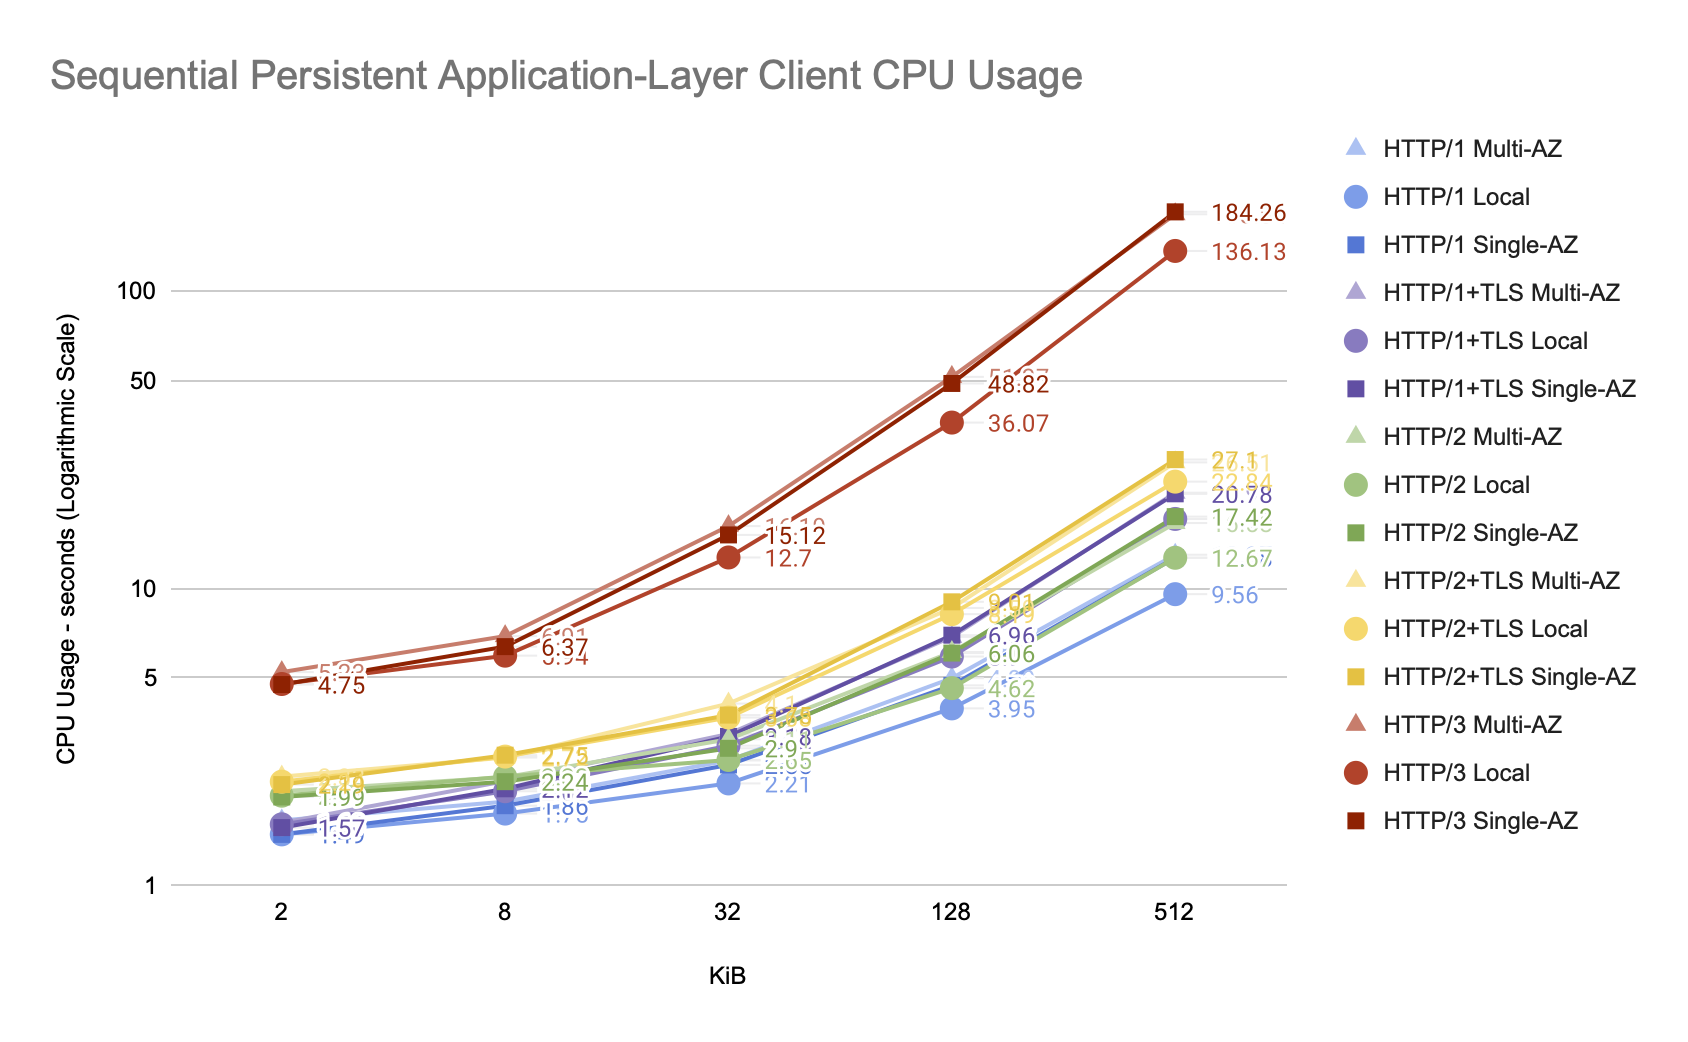
\includegraphics[width=\linewidth]{figures/charts/Sequential Persistent Application-Layer Client CPU Usage.png}
    \caption{Sequential Persistent Application-Layer Client CPU Usage}
    \label{fig:sequential_client_app_cpu}
\end{figure}
\begin{figure}[h!]
    \centering
    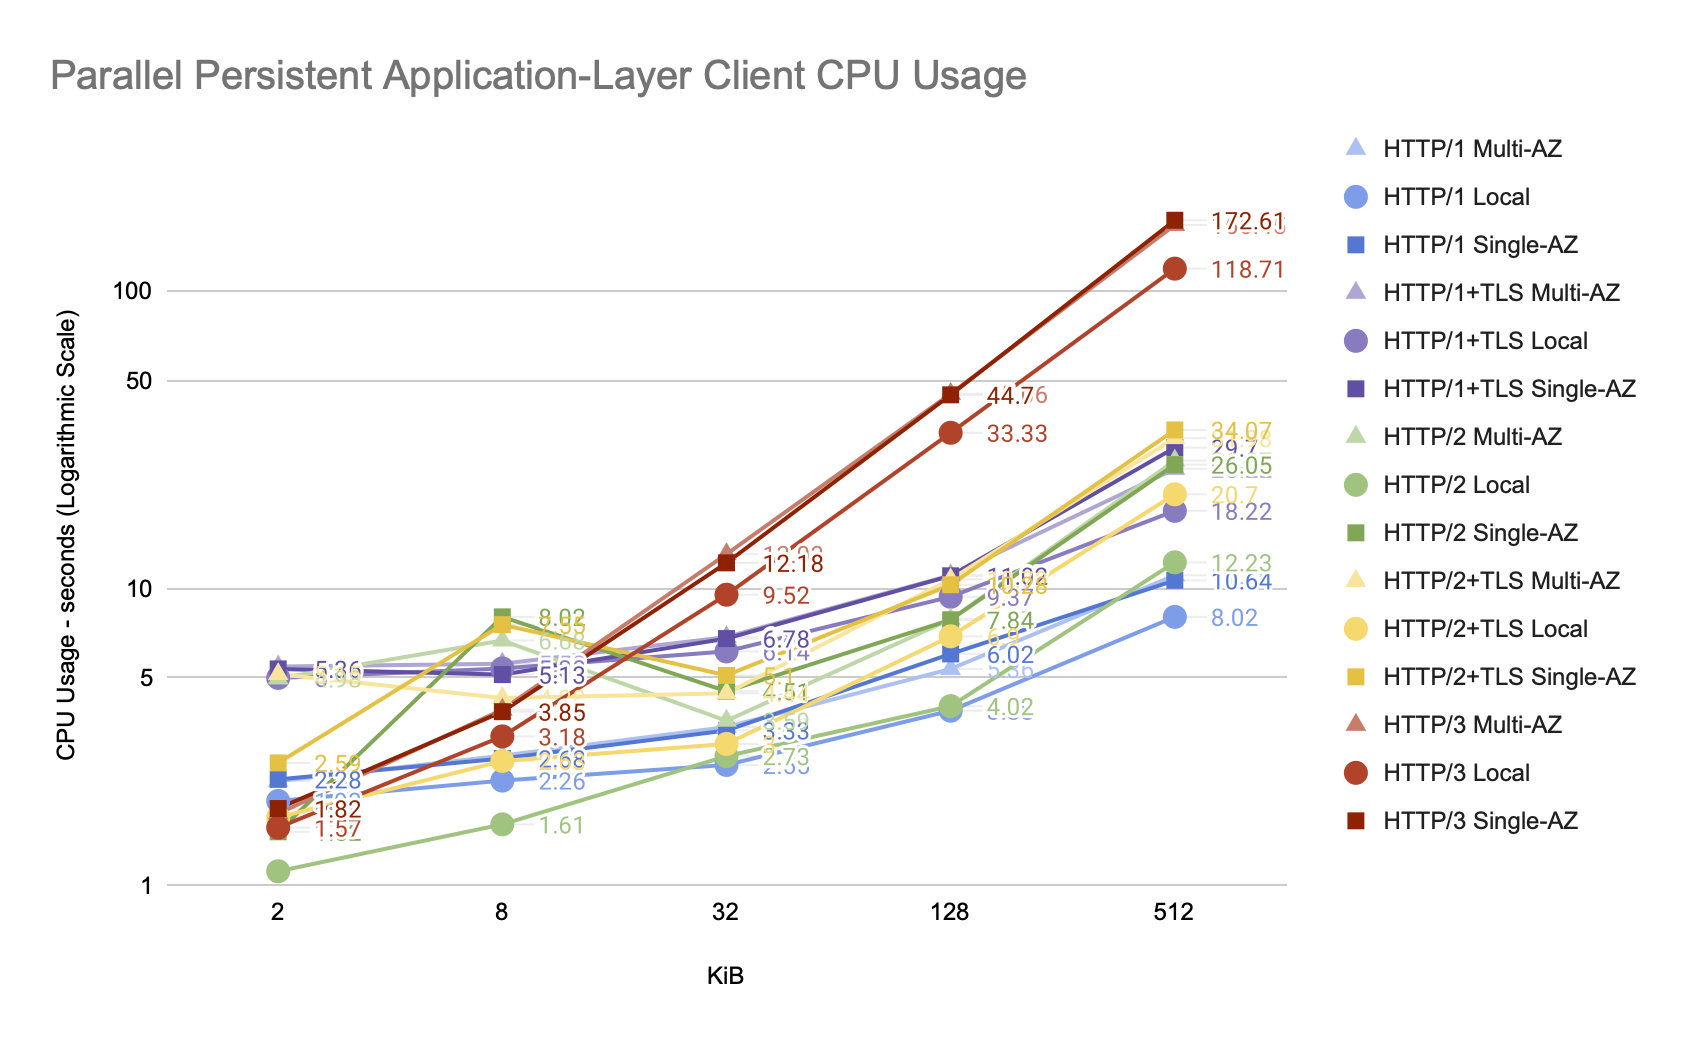
\includegraphics[width=\linewidth]{figures/charts/Parallel Persistent Application-Layer Client CPU Usage.png}
    \caption{Parallel Persistent Application-Layer Client CPU Usage}
    \label{fig:parallel_client_app_cpu}
\end{figure}

\begin{figure}[h!]
    \centering
    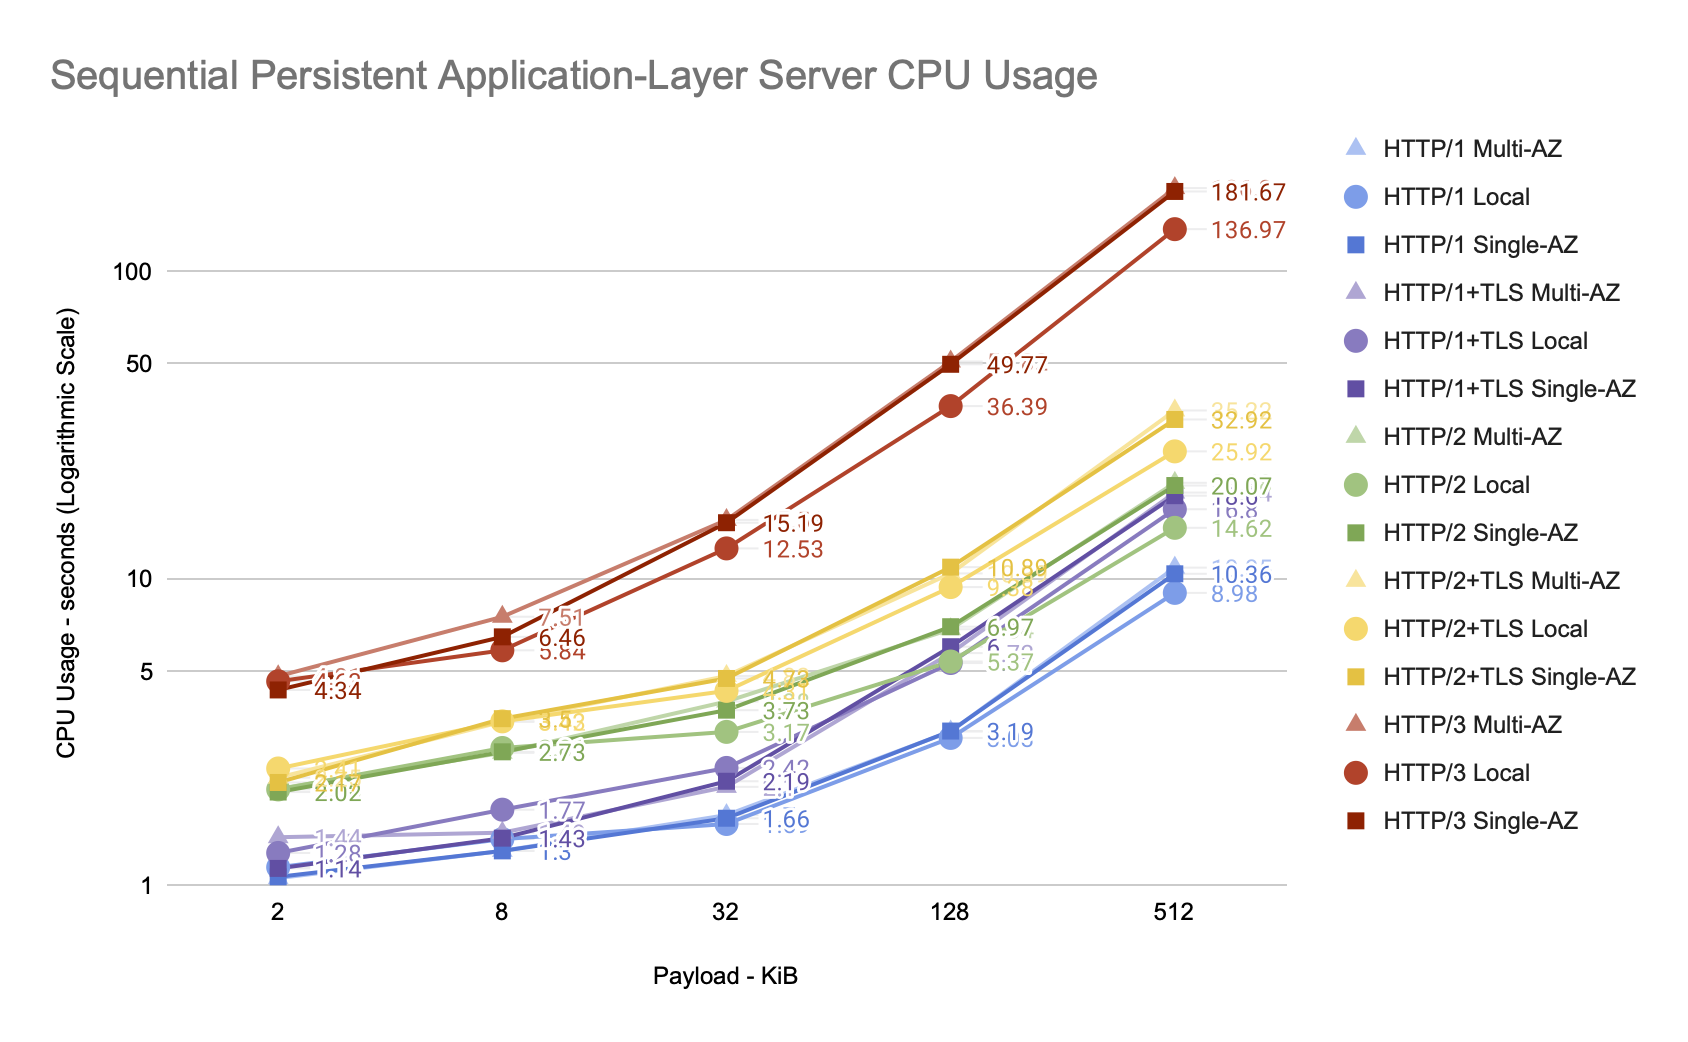
\includegraphics[width=\linewidth]{figures/charts/Sequential Persistent Application-Layer Server CPU Usage.png}
    \caption{Sequential Persistent Application-Layer Server CPU Usage}
    \label{fig:sequential_server_app_cpu}
\end{figure}
\begin{figure}[h!]
    \centering
    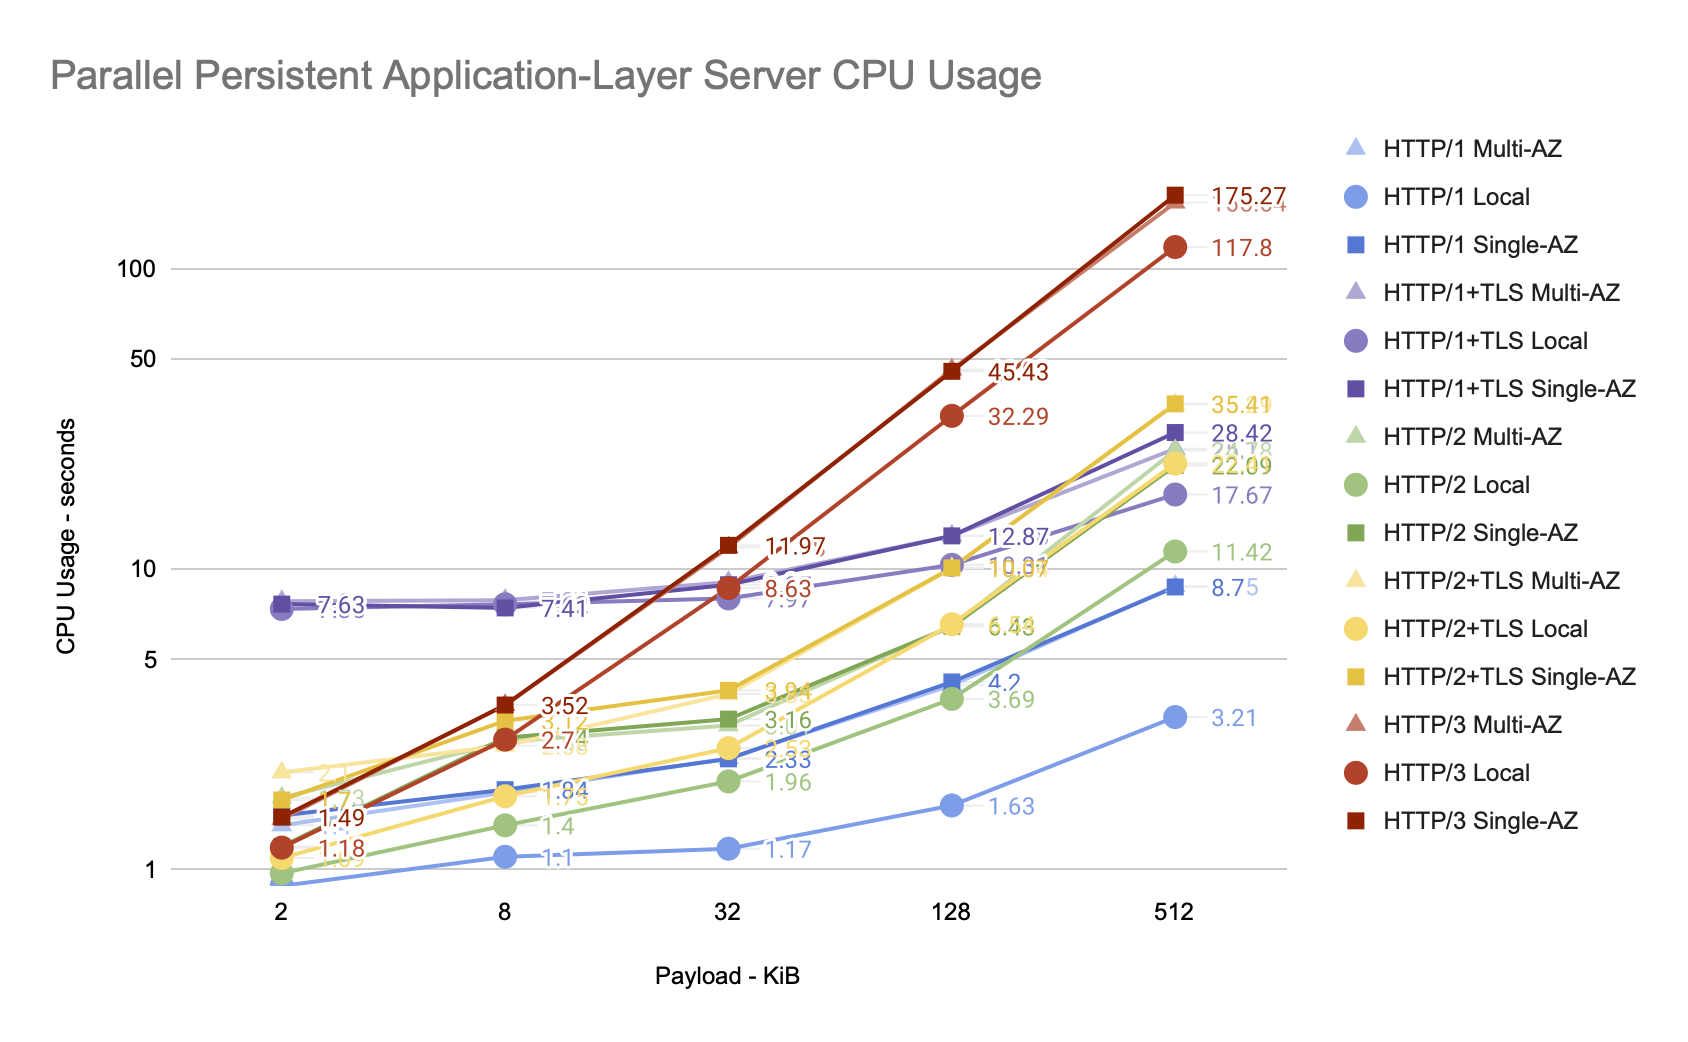
\includegraphics[width=\linewidth]{figures/charts/Parallel Persistent Application-Layer Server CPU Usage.png}
    \caption{Parallel Persistent Application-Layer Server CPU Usage}
    \label{fig:parallel_server_app_cpu}
\end{figure}

\clearpage

\subsection{Memory}

These charts represent the memory usage of clients and servers during ephemeral and persistent experiments.

These results were very similar to transport-layer experiments. \gls{http}/1 and \gls{http}/2 were the most memory efficient due to their simplicity and use of \gls{tcp} as transport protocol, which had similar results. \gls{http}/1+\gls{tls} and \gls{http}/2+\gls{tls} had increased memory usage due to \gls{tls} requirements for data encryption and \gls{tls} handshake. Finally, \gls{http}/3 had to use more memory due to QUIC’s overhead, which trades memory for efficiency.

During ephemeral experiments, Go’s garbage collector also had problems dealing with the high rate of created clients. Problem that begins worse with small data sizes, but it gets amortized as data sizes gets larger, which results in slower responses from the server, allowing Go’s garbage collector time to do its job.

\clearpage

\begin{figure}[h!]
    \centering
    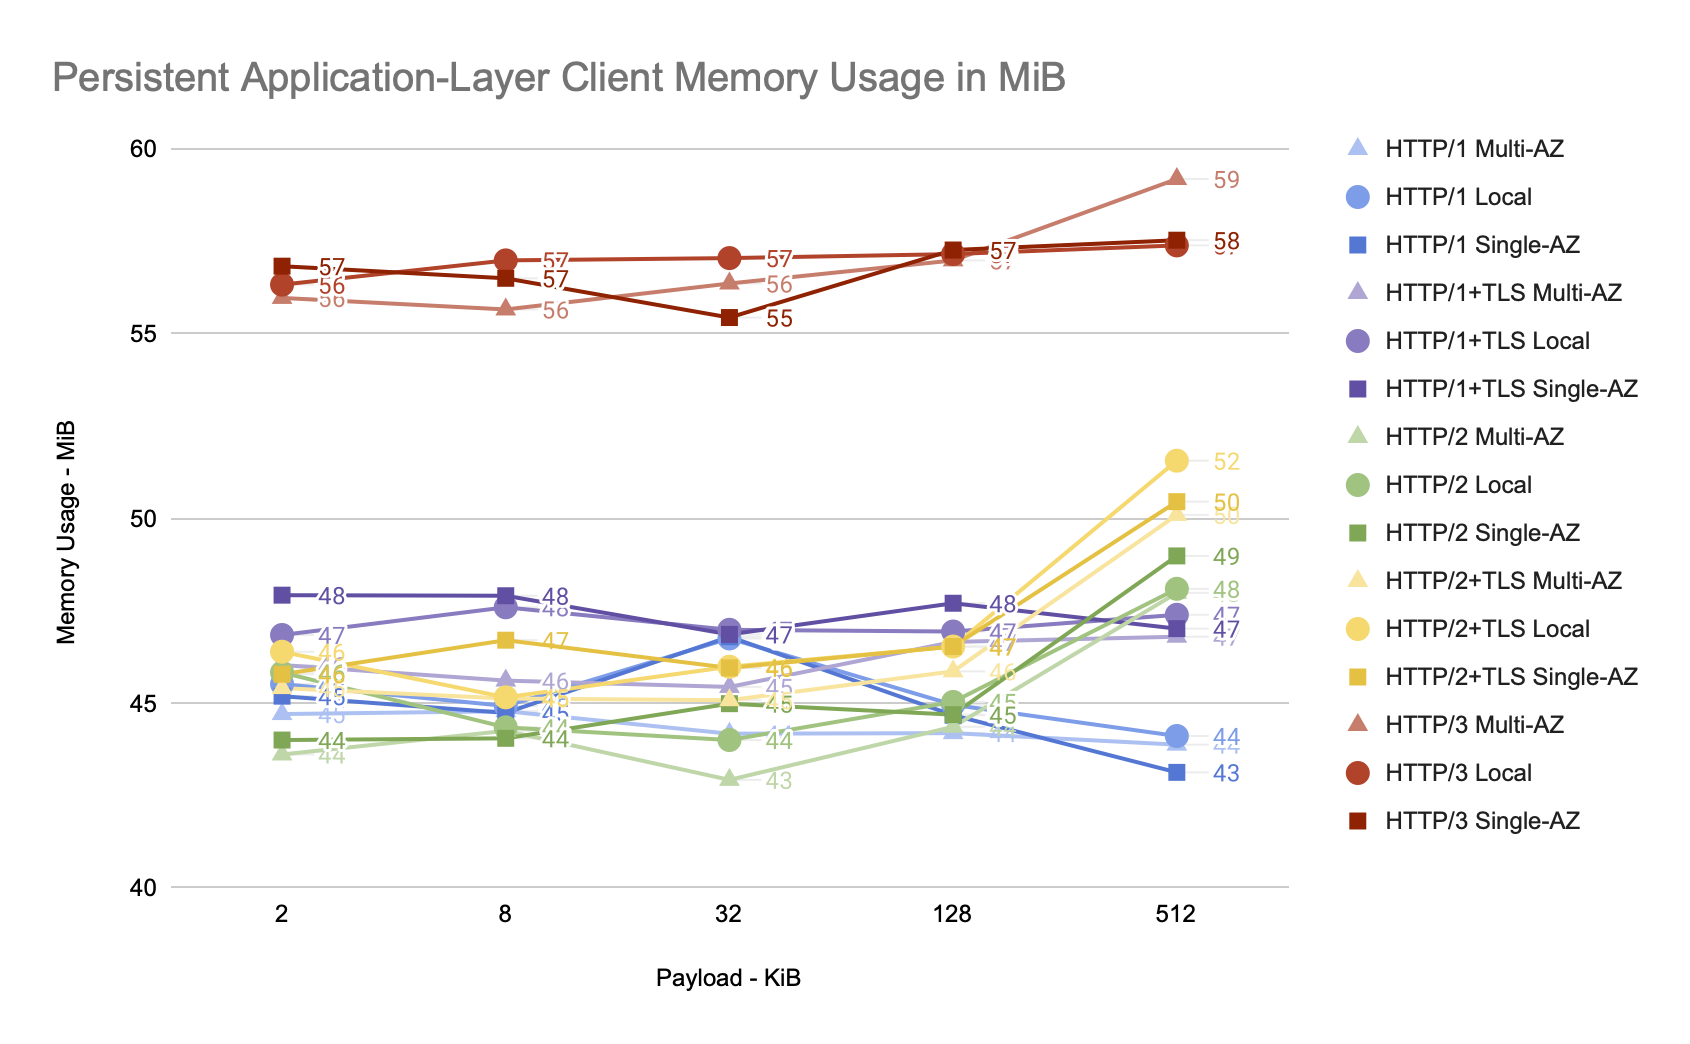
\includegraphics[width=\linewidth]{figures/charts/Persistent Application-Layer Client Memory Usage in MiB.png}
    \caption{Persistent Application-Layer Client Memory Usage in MiB}
    \label{fig:persistent_client_app_memory}
\end{figure}

\begin{figure}[h!]
    \centering
    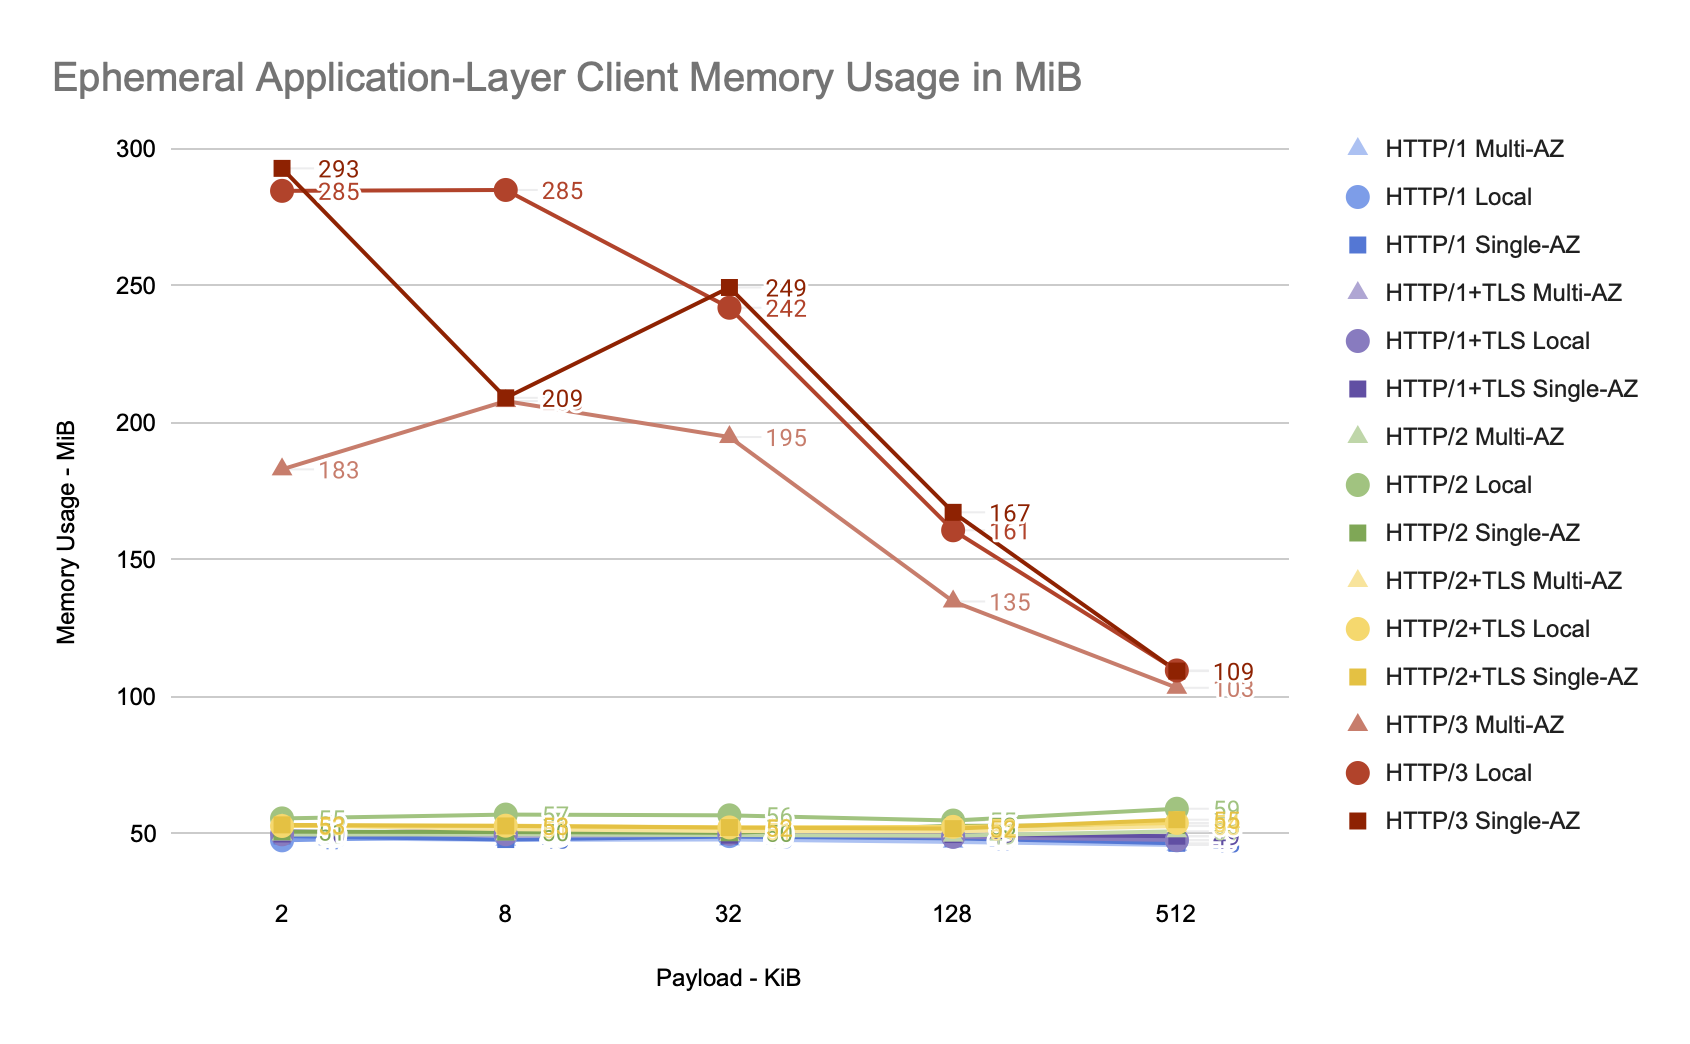
\includegraphics[width=\linewidth]{figures/charts/Ephemeral Application-Layer Client Memory Usage in MiB.png}
    \caption{Ephemeral Application-Layer Client Memory Usage in MiB}
    \label{fig:ephemeral_client_app_memory}
\end{figure}

\begin{figure}[h!]
    \centering
    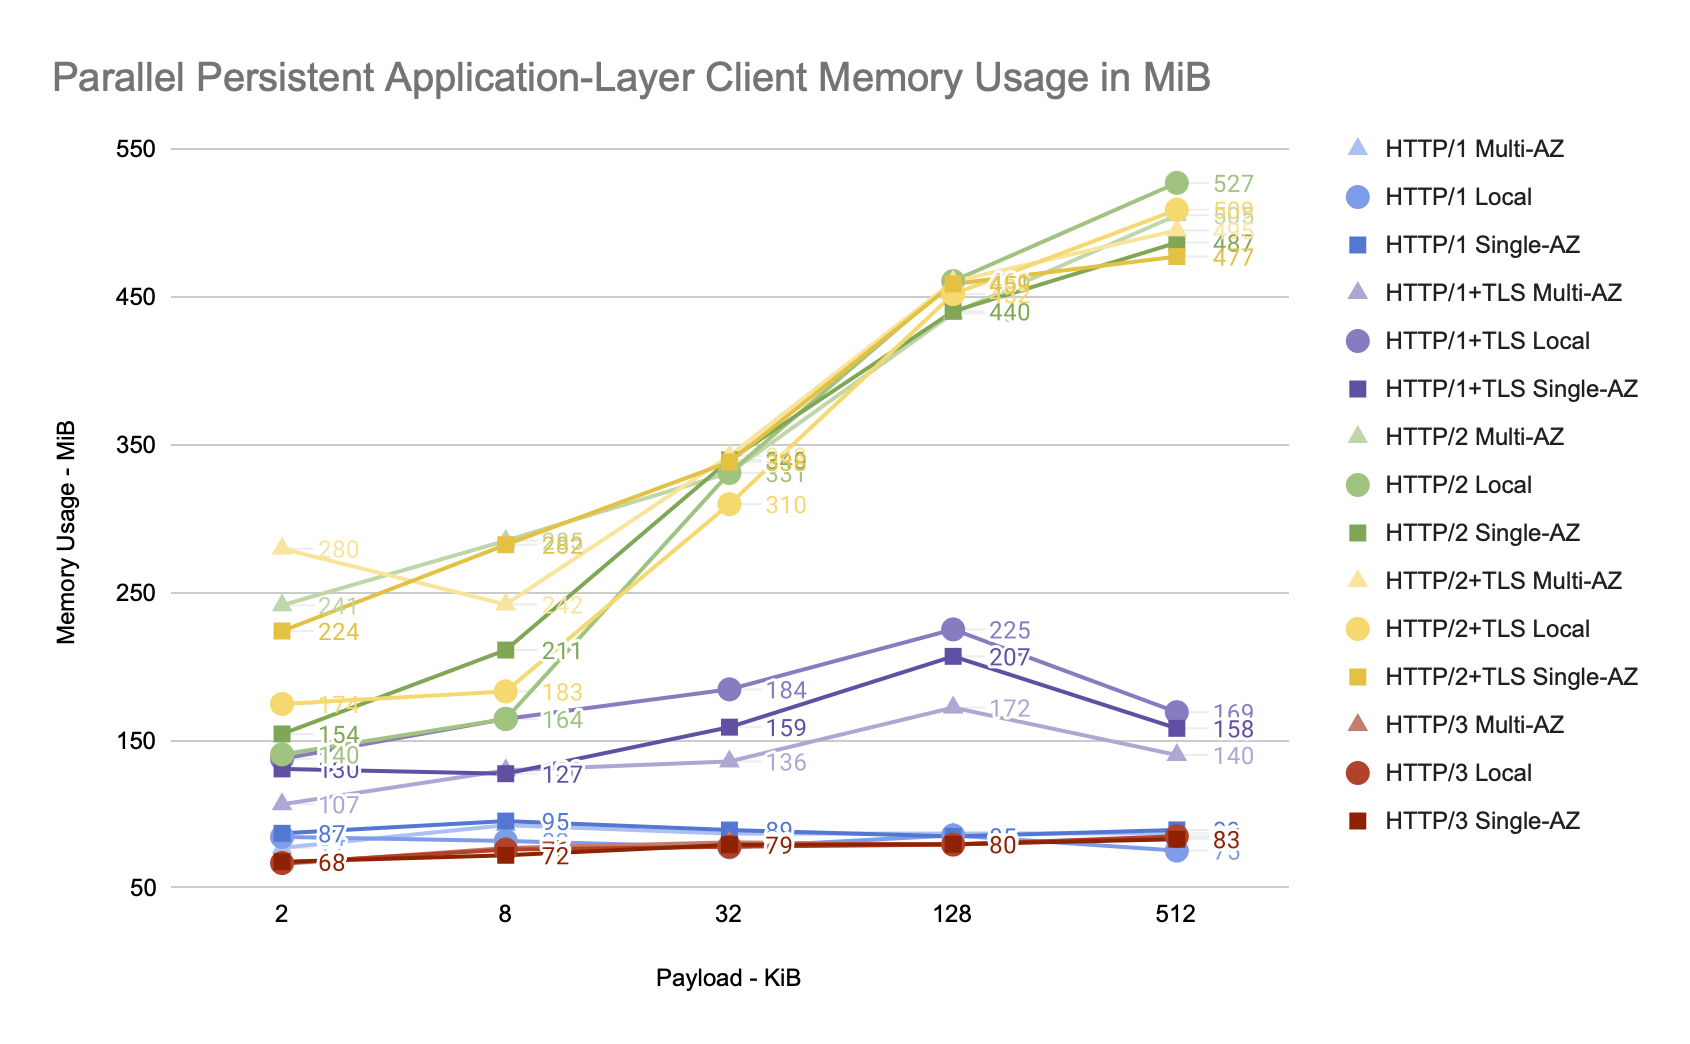
\includegraphics[width=\linewidth]{figures/charts/Parallel Persistent Application-Layer Client Memory Usage in MiB.png}
    \caption{Parallel Persistent Application-Layer Client Memory Usage in MiB}
    \label{fig:parallel_client_app_memory}
\end{figure}

\begin{figure}[h!]
    \centering
    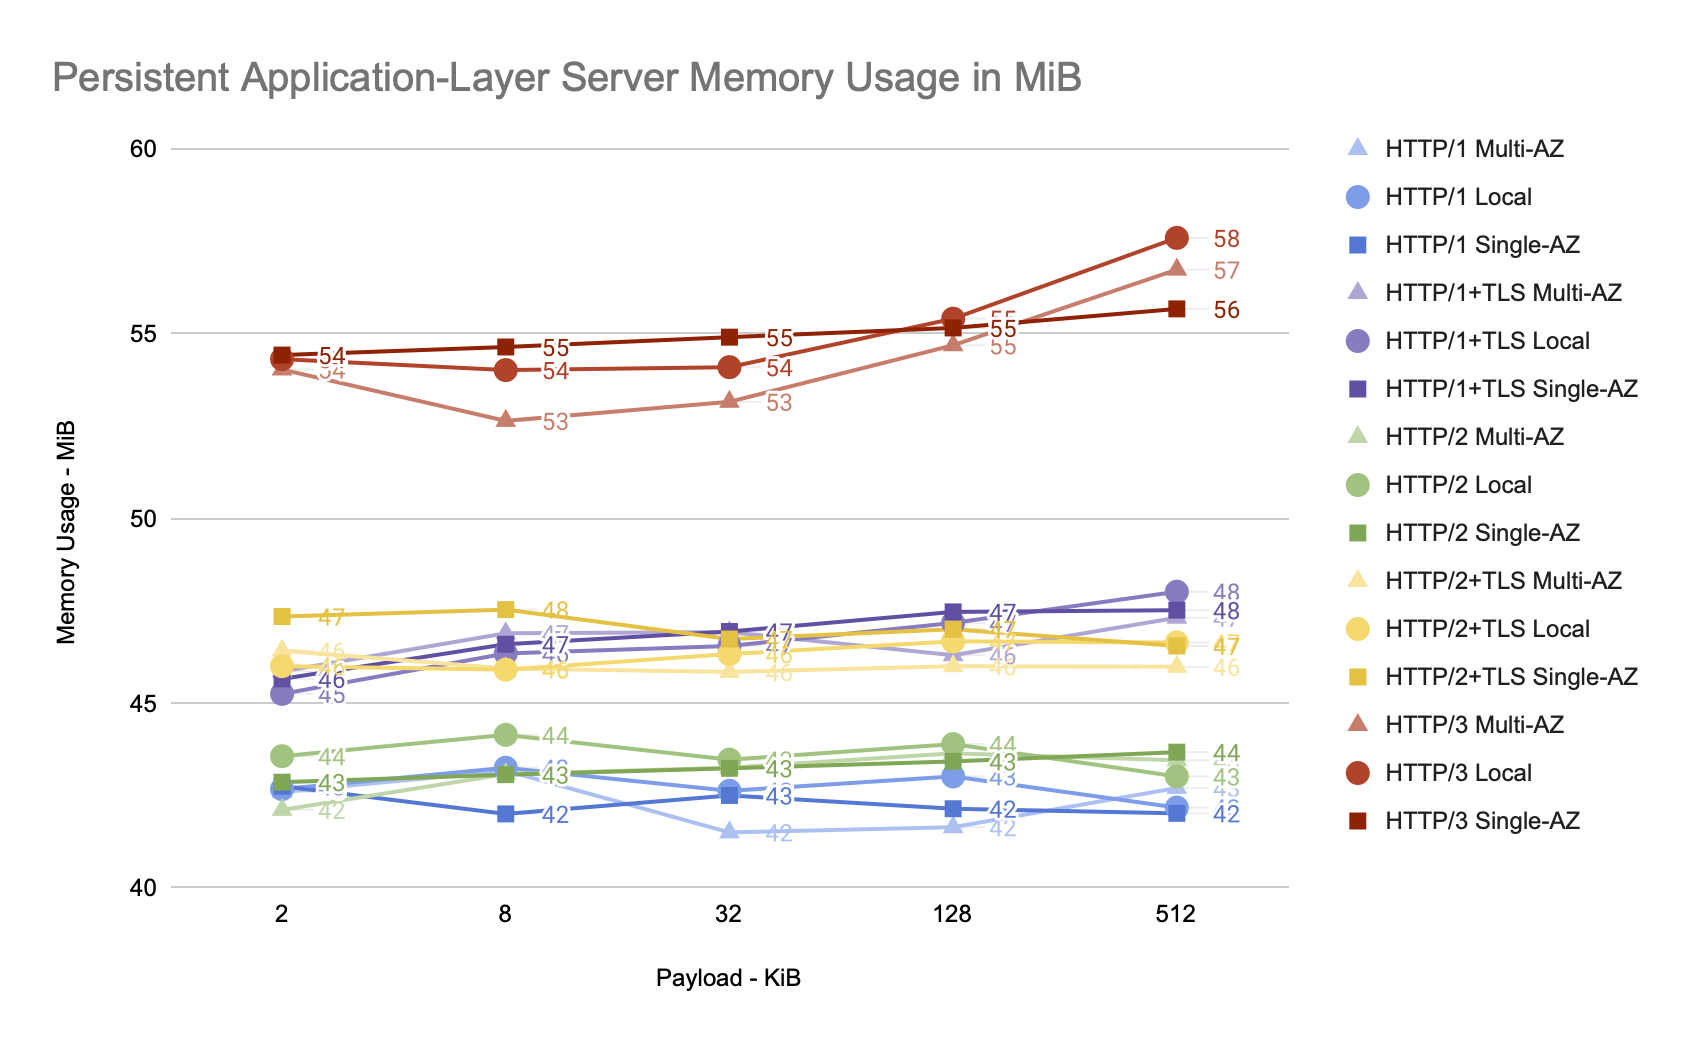
\includegraphics[width=\linewidth]{figures/charts/Persistent Application-Layer Server Memory Usage in MiB.png}
    \caption{Persistent Application-Layer Server Memory Usage in MiB}
    \label{fig:persistent_server_app_memory}
\end{figure}

\begin{figure}[h!]
    \centering
    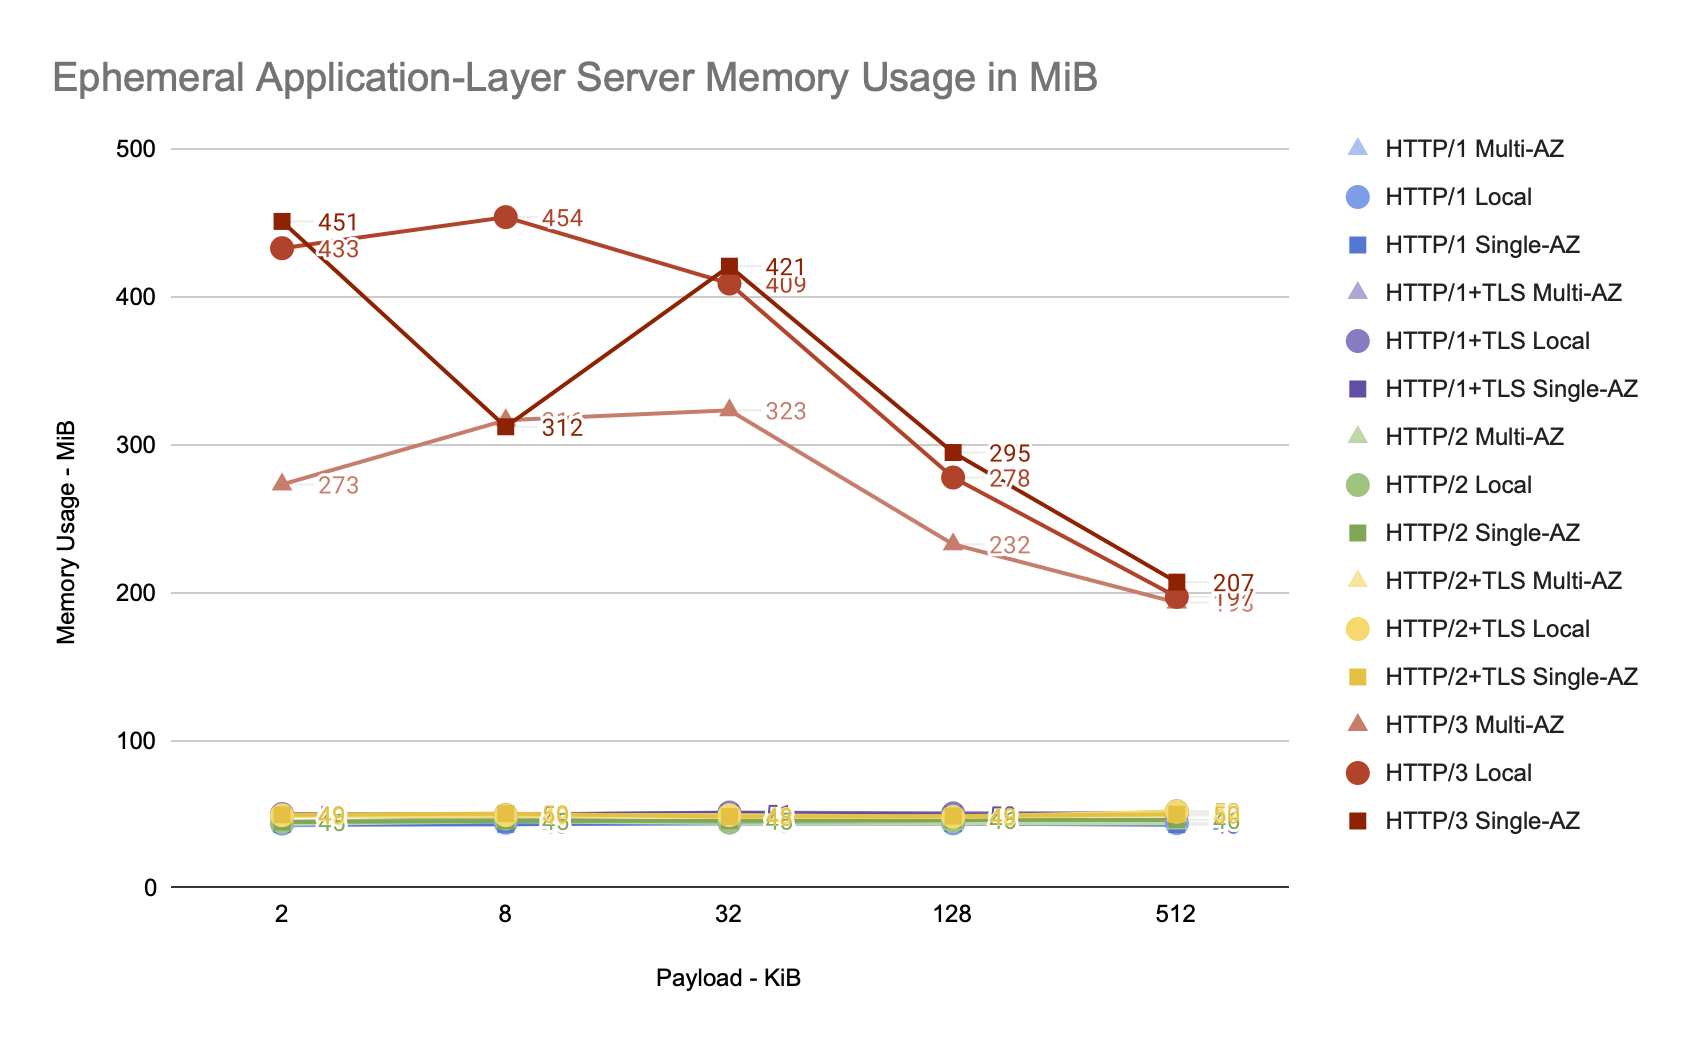
\includegraphics[width=\linewidth]{figures/charts/Ephemeral Application-Layer Server Memory Usage in MiB.png}
    \caption{Ephemeral Application-Layer Server Memory Usage in MiB}
    \label{fig:ephemeral_server_app_memory}
\end{figure}

\begin{figure}[h!]
    \centering
    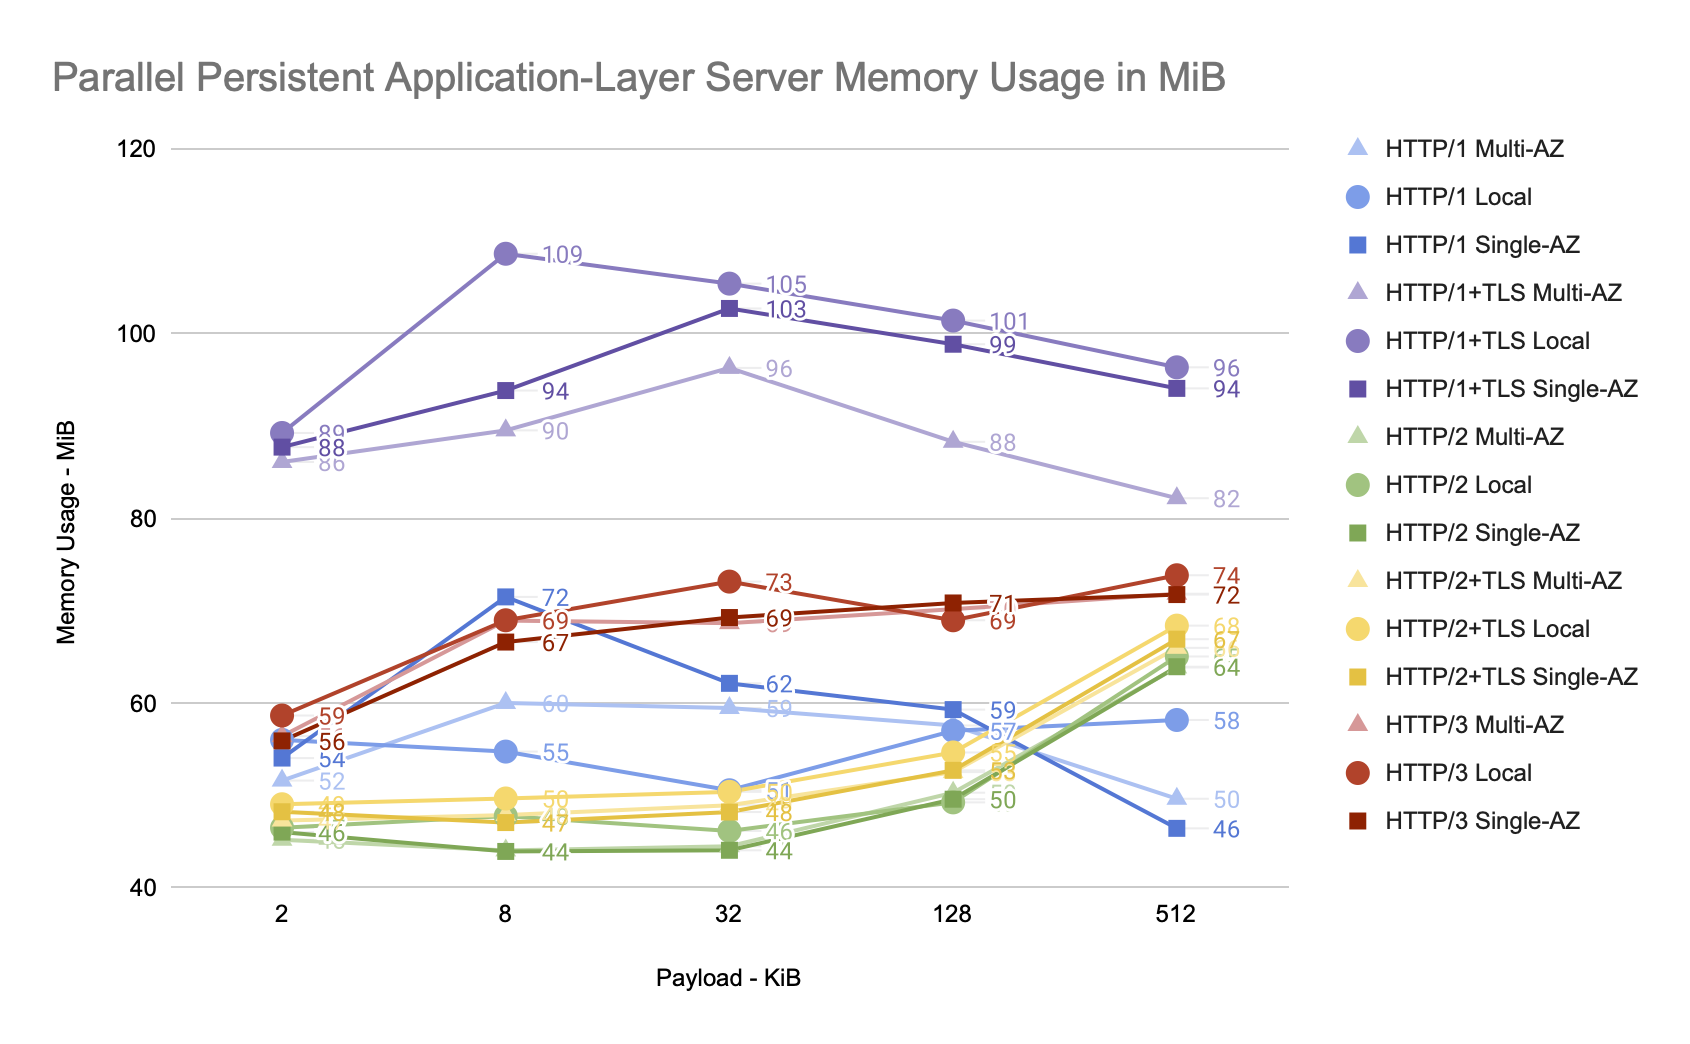
\includegraphics[width=\linewidth]{figures/charts/Parallel Persistent Application-Layer Server Memory Usage in MiB.png}
    \caption{Parallel Persistent Application-Layer Server Memory Usage in MiB}
    \label{fig:parallel_server_app_memory}
\end{figure}

\clearpage

\section{Cost}

<INSERT>

\clearpage

\subsection{Summary}

<INSERT>

\clearpage

\section{Conclusion}

QUIC has proven to be a better alternative to TCP on unreliable networks, addressing multiple problems of TCP when handling packet loss. Another advantage is the incorporation of the TLS protocol, forcing all connections to be encrypted. Relying on UDP and running on user-space, makes it compatible with existing network equipment and can be implemented by any application.

However, the experiments showed that on a cloud environment, where the network is extremely reliable, QUIC performed worse than TCP. Tuning kernel parameters to improve UDP traffic did not bring a significant advantage to QUIC. Additionally, it was also observed that QUIC requires more compute resources when compared to other protocols, increasing the cost of applications that use it.

HTTP/3, which is based on QUIC, suffers from similar problems and showed poor performance for interservice communication. It was not possible to push the protocol to its full potential, as most of its features are better used by a browser rather than in a cloud environment.

QUIC and HTTP/3 are still a great solution for user-facing applications, improving the experience for the end-user with an extra cost for the server. But it doesn’t have a great fit with internal networks, where packet loss is extremely low. In that case it is better to use more traditional protocols that rely on TCP, even with TLS as an additional layer.

The protocol is relatively new and it’s possible that in the future it becomes more competitive in reliable networks. In the meanwhile, TCP/TLS is a great solution that has been supporting the majority of the Internet for years, and it is not going away anytime soon.

\clearpage


\bibliographystyle{plain}
\bibliography{refs}
\clearpage

\printglossary[type=\acronymtype]
\clearpage

\end{document}
